\documentclass[a4paper,12pt, twoside]{book}

%typo générale
\usepackage[margin=2cm]{geometry}
\usepackage{setspace}
\setstretch{1,25}
\setlength\parindent{1cm}
\parskip=9pt
\usepackage{lipsum}
%\usepackage{emptypage}

%config images et légende
\usepackage{graphicx}
\usepackage{subfigure}
\graphicspath{{images_memoire/}}
\usepackage[justification=centering]{caption}
\usepackage{float}
%couleur
\usepackage[dvipsnames]{xcolor}
\usepackage{minted}

% encodage
\usepackage{inputenc}
\usepackage{fontspec}
\usepackage[english,french]{babel}

%création hyperliens
\usepackage{hyperref}
\hypersetup{
urlcolor= blue,
linkcolor= blue,
pdfauthor={Anne Bugner},
pdftitle={memoireannebugner2023},
pdfsubject={mastertnah},
pdfkeywords={omekas} {mapping} {nosql database} {python} {wamp} {semantic web} {agorha}}

%annexes
\usepackage{appendix}

%bibliographie
\usepackage[backend=biber,style=enc,sorting=nyt]{biblatex}
\usepackage{csquotes}
\FrenchFootnotes
\AddThinSpaceBeforeFootnotes
\addbibresource{réflexionshistoriographiques.bib}
\addbibresource{esthétique.bib}
\addbibresource{travauxhistoire.bib}
\addbibresource{analysescontemporaines.bib}
\addbibresource{gestiondebasesdedonnées.bib}
\addbibresource{webdocuments.bib}
\addbibresource{aideoutils.bib}
\addbibresource{vocabulaires.bib}
\addbibresource{gestiond'unprojetculturelnumérique.bib}
\nocite{*}

%\DeclareSourcemap{
%\maps[datatype=bibtex]{
%\map[overwrite]{
%\perdatasource{réflexionshistoriographiques.bib}
%\step[fieldset=keywords, fieldvalue={,htg}, append]}
%\map[overwrite]{
%\perdatasource{esthétique.bib}
%\step[fieldset=keywords, fieldvalue={,est}, append]}
%\map[overwrite]{
%\perdatasource{travauxhistoire.bib}
%\step[fieldset=keywords, fieldvalue={,pig}, append]}
%\map[overwrite]{
%\perdatasource{analysescontemporaines.bib}
%\step[fieldset=keywords, fieldvalue={,ana}, append]}
%\map[overwrite]{
%\perdatasource{gestiondebasesdedonnées.bib}
%\step[fieldset=keywords, fieldvalue={,db}, append]}
%\map[overwrite]{
%\perdatasource{webdocuments.bib}
%\step[fieldset=keywords, fieldvalue={,web}, append]}
%\map[overwrite]{
%\perdatasource{aideoutils.bib}
%\step[fieldset=keywords, fieldvalue={,cod}, append]}
%\map[overwrite]{
%\perdatasource{vocabulaires.bib}
%\step[fieldset=keywords, fieldvalue={,voc}, append]}
%\map[overwrite]{
%\perdatasource{gestiond'unprojetculturelnumérique.bib}
%\step[fieldset=keywords, fieldvalue={,pro}, append]}
%}
%}

%inclusion de pdfs
\usepackage{lscape}
\usepackage{pdflscape}
\usepackage[final]{pdfpages} 

%renews
\definecolor{teal1}{RGB}{0, 139, 139}
\definecolor{teal2}{RGB}{32, 178, 170}
\definecolor{teal3}{RGB}{0, 128, 128}
\definecolor{urlblue}{RGB}{0, 0, 139}
\definecolor{greencode}{RGB}{46, 139, 87}
\definecolor{graycode}{RGB}{162, 137, 128}
\definecolor{codetab}{RGB}{252, 244, 241}

\renewcommand{\FrenchLabelItem}{\textbullet}

\renewcommand{\cleardoublepage}{\clearpage\thispagestyle{empty}\newpage}

\author{Anne Bugner}
\title{memoiretnah}
\date{2023}

\begin{document}

\begin{titlepage}

\begin{center}

        ÉCOLE NATIONALE DES CHARTES\\
        \textsc{Master Techniques Numériques Appliquées à l'Histoire}\\
        \medskip
        \textsc{Année 2023}  

%Ceci est une ligne
\begin{center}\rule{2cm}{0.02cm}\end{center}

\bigskip
\bigskip
\bigskip

Anne \textsc{Bugner}

\bigskip
\bigskip
\bigskip
\bigskip
\bigskip

\begin{Large}
\textcolor{greencode}{\textbf{D'Agorha à Omeka S}}\\    
\end{Large}
\bigskip
\bigskip
\begin{large}
    \textcolor{teal1}{\textbf{Transformer deux bases de données d’exposition des matériaux de la couleur dans l’histoire de l’art en deux bases d’exploitation automatique à destination de publics différenciés}}
\end{large}

\begin{figure}[!h]
    \centering
    \includegraphics[height=5.6 cm]{couv.png}
    \caption*{Manuscrit prêt pour analyse XRF à la BnF Richelieu, lundi 5 juin 2023.}
\end{figure}

\large\textbf{Stage de fin d'études}\\
\medskip
\textbf{Bibliothèque Nationale de France, département des Manuscrits}\\
Projet de recherche \textit{«~La couleur~: artefacts, matière et cognition~»}\\

\medskip
03/04/2023 – 28/07/2023

\vfill

Direction Charlotte \textsc{Denoël} (BnF), Emmanuelle \textsc{Bermès} (ENC)
\end{center}
\end{titlepage}

\frontmatter

\clearemptydoublepage
\chapter*{Résumé}

La BnF et l’INHA développent en partenariat une ressource documentaire recensant les matériaux constitutifs des œuvres d’art picturales, relevant des spécialités respectives des expert·es scientifiques (icônes peintes dans l’espace méditerranéen, manuscrits médiévaux enluminés), détaillant en particulier l’identification des pigments constituant les couleurs, et leur assimilation à un élément visuel significatif.

\medskip

L’objectif du projet est de proposer deux bases de données interactives, permettant de croiser les considérations matérielles, historiques et esthétiques, une première version étant en cours de production sur le site Agorha.

\medskip

Ce stage intervient dans le cadre de l’avant-dernier volet du projet~: celui de la conception d’une deuxième version de ces bases de données, axée sur le traitement automatisé des informations, en vue de la production de représentations graphiques à la demande. Il se concentre sur la configuration du logiciel Omeka S, la caractérisation et l’extraction des données hébergées sur Agorha, et leur réorganisation pour Omeka S. Cela se traduit par l'installation du serveur virtuel WAMP, et l'automatisation des tâches par script Python.

\vfill

\textbf{Mots-clés}~: Histoire de l'art, histoire médiévale, Analyses physico-chimiques, Bases de données NoSQL, \textit{Mapping}, Web sémantique, Agorha, Omeka S, Python, MariaDB, WAMP.

\bigskip

\textbf{Informations bibiographiques} : Anne \textsc{Bugner}, \textit{D’Agorha à Omeka S~: Transformer deux bases de données d’exposition des matériaux de la couleur dans l’histoire de l’art en deux bases d’exploitation automatique à destination de publics différenciés}, mémoire de master \og Technologies numériques appliquées à l'histoire\fg , dir. Emmanuelle \textsc{Bermès}, Charlotte \textsc{Denoël}, École Nationale des Chartes, 2023.

\clearemptydoublepage
\chapter*{Remerciements}
\addcontentsline{toc}{chapter}{Remerciements}

Je souhaiterais exprimer toute ma gratitude envers M\textsuperscript{me} Charlotte \textsc{Denoël} – directrice du service des manuscrits médiévaux de la BnF et à l’initiative de ce stage de fin d’études – pour la qualité de l’accueil et du suivi dont j’ai bénéficié, mais également pour le soin de me transmettre un peu de son expertise d’histoire de l’art médiéval et de m’intégrer aux réunions de service, connaissant mon intention de travailler pour la conservation des bibliothèques à terme. Ma reconnaissance va également à M\textsuperscript{me} Sigrid \textsc{Mirabaud}, co-directrice scientifique du projet La fabrique de l’art du côté de l’INHA, ainsi qu’à Federico \textsc{Nurra} et Chloé \textsc{Pochon}, du Service Numérique de la Recherche, pour leur disponibilité, leurs encouragements et leur confiance renouvelée. Elle va également à ma coéquipière sur ce projet, Teresa \textsc{Knapowska}, ancienne du master TNAH et mentor précieuse d’organisation et de gentillesse.

Au même titre, je remercie M\textsuperscript{me} Emmanuelle \textsc{Bermès}, responsable pédagogique de notre master et tutrice de ce stage en tant que spécialiste des données documentaires en bibliothèque. Je la remercie pour son détermination à trouver à chacun·e un stage en cohérence avec ses choix d’orientation, proposer un suivi personnalisé, et sa bienveillance constante tout au long de cette année agitée.

Je remercie M. Gennaro \textsc{Toscano} d’avoir accepté de lire et critiquer ce mémoire.

Je remercie l’équipe pédagogique de notre master, et en particulier MM. Olivier \textsc{Canteaut} et Pearce \textsc{Groover}, pour leur présence, leur patience et leurs retours très détaillés sur mes travaux de M1.

Je remercie mes coéquipier·es de master pour les nombreux moments de soutien et de rires, en souhaitant que leur futur professionnel valorise leurs talents de jeunes chercheur·euses et ingénieur·es à la hauteur des efforts fournis pour maîtriser tant de techniques en quelques mois.

Quand bien même cela reste symbolique, je tiens aussi que soient remercié·es M. Olivier \textsc{Piffault} pour m’avoir généreusement ouvert les portes du département de la Conservation de la BnF à l’été 2020, et par là fait rencontrer M\textsuperscript{me} Célia \textsc{Cabane} (Coordination informatique), qui m’initia aux problématiques des données de la conservation, M. Emmanuel \textsc{Jaillet} (département des Métadonnées), qui me dispensa une impressionnante formation accélérée en matière de catalogage en modèle entités-relations, de Web sémantique et de migration de bases de données, et enfin M\textsuperscript{me} Mathilde \textsc{Dutertre} (service Numérisation), ancienne du master TNAH, qui me parla de cette formation, et marqua le début de cette histoire.

\begin{quote}
\small{Pour finir, ma gratitude va droit aux nombreux soutiens lors des galères improbables du quotidien, parmi lesquels – par ordre d’apparition – les infatigables sentinelles Delphine \textsc{Bugner} et Damien \textsc{Bonnelle}, le seigneur du droit de la fonction publique et des installations Linux artisanales Louis \textsc{Hemmer-Petitcolas}, le garant des puzzles et scripts Python dépareillés Théophile \textsc{Héliot}, la cohorte des docteur·es toutes disciplines confondues Tito \textsc{Nguyen}, Bastien \textsc{Dumont}, Béranger \textsc{Seguin}, Oleg \textsc{Rouditch-Pergola} et Svetoslava \textsc{Nikolaeva}, la très combative avocate du droit immobilier Alina \textsc{Boutchenik}, le duo des lumières en salles de lecture de la BnF Manon \textsc{Bertaux} et Hugo \textsc{Poux}, la bonne fée du 12\textsuperscript{e} arrondissement parisien Murielle {Marussig}, et enfin l’agrégatif assoiffé de bibliographies qui se reconnaîtra dans l’appellation « moine copiste » page suivante, Merwan \textsc{Touati}.}
\end{quote}

\clearemptydoublepage
\chapter*{Introduction}
\addcontentsline{toc}{chapter}{Introduction}

\begin{flushright}
\scriptsize\textcolor{teal3}{«~Je m’approchai et aperçus sur la page quatre bandes de couleur différente, jaune, cinabre, bleu turquin et terre brûlée. S’y détachait une bête horrible à voir, un grand dragon avec dix têtes qui de sa queue entraînait à sa suite les étoiles du ciel, et les faisait s’abîmer sur la terre…~»}\\

\medskip

\textcolor{teal3}{Umberto \textsc{Eco}, \textit{Le Nom de la Rose}, «~Deuxième jour~», traduction de Jean-Noël \textsc{Schifano}, 1982.}
\end{flushright}
\normalsize
\bigskip

Ce n’est guère un hasard si le très polyvalent Umberto \textsc{Eco}, en concevant l’intrigue du Nom de la Rose en romancier d’aventure, ses dialogues en philosophe et ses décors en peintre géomètre, aborde la description de ses enluminures en sémiologue. Les livres de la bibliothèque interdite entrent dans le récit autant par leurs éléments visuels que par les brèves citations de leur contenu ; ils sont soigneusement découpés en motifs, plans, couleurs et matériaux, suggérant les contours d’une grammaire visuelle familière aux doctes moines copistes. En effet, le recours aux aplats unis, compositions irréalistes ou profusions de motifs géométriques pour les décors enluminés relève de la représentation systématique d’un concept théologique, à un degré comparable à l’art abstrait de notre dernier siècle.

Les couleurs, sous la plume érudite d’Eco, possèdent leur nom propre \scriptsize\textit{(«~bleu turquin~»)}\normalsize, qui se trouve parfois être directement leur matériau \scriptsize\textit{(«~orpiment~», «~terre brûlée~»)}\normalsize, ce qui suggère que le narrateur a été éduqué à les singulariser. Elles ont une valeur en soi. Celle de du prix de leur fabrication, certes, mais surtout celle du savoir à l’œuvre pour leur transformation, qui relève d’une tradition artisanale propre à une communauté. C’est pourquoi on peut estimer que la mention d’une origine géographique, pour nommer une couleur, participe à la distinction de centres artisanaux dynamiques et de ses réseaux commerciaux liés.

Étudier les couleurs d’une œuvre artistique, à la fois dans leur composition matérielle, leur technique d’exécution et le motif visuel qu’elles composent, fournit ainsi des informations quant à la circulation de produits dans un espace donné, l’organisation sociale du travail d’artiste, la transmission des savoirs, l’élaboration d’une grammaire symbolique et des styles esthétiques. Bien des disciplines scientifiques s’y intéressent~: histoire et histoire de l’art, ethnologie, anthropologie, philologie, archéologie, philosophie, physique, chimie, sciences du patrimoine en général... Aussi l’analyse de la composition des couleurs constitue-t-elle aujourd’hui un terrain d’enquête pluridisciplinaire privilégié, dans l’espoir que des campagnes d’analyses complexes à organiser servent au plus vaste éventail de professionnel·les possible. Or comment centraliser des informations issues de provenances diverses, et ce d’une manière suffisamment transparente pour permettre leur réutilisation dans le cadre de projets scientifiques tout autres~?

L’idéal serait un outil qui combinât les données physico-chimiques issues des campagnes d’analyses avec les données documentaires descriptives des œuvres elles-mêmes~: il associerait les matériaux et techniques à des dates de création, ou des localisations géographiques. L’adjonction de d’une indexation des éléments visuels présents ouvrirait également la perspective d’analyses sémantiques. L’accès à des collections variées, depuis plusieurs institutions, rendrait possible les comparaisons entre corpus similaires (par leur type d’œuvre, leur datation, leurs provenances), voire les approches quantitatives. Or un tel outil offrant d’interroger ensemble couleurs, motifs iconographiques, matériaux et œuvres, n’existe pas encore.

C’est dans l’espoir qu’il voie le jour que la BnF et l’INHA ont initié de concert un programme de recherche en trois ans~: \textit{«~La couleur~: artefacts, matière et cognition~»}, dont le présent stage constitue l’avant-dernier volet. La plate-forme d’outils d’aide à la recherche numériques de l’INHA, Agorha, héberge deux bases de données originales~: \textit{La fabrique matérielle du visuel. Panneaux peints en Méditerranée, XIIIe-XVIe siècles}, dépendant de l’équipe scientifique de l’INHA, et \textit{La fabrique de l'art. Couleurs et matériaux de l'enluminure}, dépendant de celle de la BnF. Elles sont alimentées, à fréquence régulière, de notices compilant trois types d’informations~: les matériaux recensés (que ce soit pour leurs couches picturales, leurs supports, leurs couches de finition, ainsi que leur état de conservation) les informations d’ordre documentaire~; et les précisions quant à leur fiabilité générale et leur méthode d’obtention. La création de quatre thesaurus (\textsf{Couleur, Technique, Caractéristique, Matériau}) a permis de structurer ces informations de manière harmonisée dans leur diversité. Car si les corpus d’œuvres choisies sont encore restreints (manuscrits médiévaux, panneaux d’art sacré), la base ambitionne de traiter de toutes les aires géographiques et temporelles, et de recenser des techniques artisanales spécifiques.

La mission de ce stage n’était pas de participer à l’obtention de ces données, ni d’élaborer un vocabulaire de description \textit{matérielle} inédit pour leur compréhension. Ces étapes-là ont déjà été effectuées et validées par le comité de pilotage, en les personnes de Mmes Sigrid \textsc{Mirabaud} (chercheuse pensionnaire de l’INHA) et Charlotte \textsc{Denoël} (cheffe de service des Manuscrits médiévaux à la BnF). Les deux bases de données hébergées sur Agorha sont riches de centaines de notices, quoi que visibles encore aux seul.es contributeur·ices. Toutefois, si les matériaux recensés au sein d’une œuvre y sont décrits dans le détail, ils n’en restent pas moins dépendants d’une notice où ils ne sont pas au premier plan. Il est encore difficile de les interroger tous ensemble, de comparer leurs caractéristiques, ou d’esquisser les évolutions des fonctions picturales qui leur sont assignées.

Ce stage entend réorganiser ces données au sein de deux nouvelles bases, afin que tous les niveaux d’information d’une notice puissent faire l’objet de requêtes directes et produire des représentations graphiques de qualité, dans le but de faire émerger des constats que les tenant·es d’une discipline n’auraient pas obtenus seul·es, de transmettre à chaque communauté professionnelle les informations des autres. Naturellement, cette perspective s’accompagne de son propre lot de questionnements~: quels sont ces communautés qui constitueraient les publics utilisateurs de nos bases~? Quels types de données recherchent-elles, et pour quels usages~? Quelles sont leurs habitudes documentaires~? Comment les concilier, tout en les emmenant vers des terrains moins familiers~? La configuration des bases de données en dépend~: quelles informations doivent ressortir en priorité~? Comment les organiser en notices, blocs et champs, pour ensuite préparer les requêtes des moteurs de recherche, et les visualisations graphiques des résultats~? Y répondre avec acuité nécessite un travail d’enquête fourni, malheureusement incompatible avec la durée d’un stage de fin d’études. Il fut donc décidé d’initier un simple premier prototype, dont les paramètres seraient modifiables à l’envi.

Ce stage s’est donc attelé à l’initiation des deux bases dites «~d’exploitation~» à partir de celles développées sur Agorha. Les chantiers principaux ont consisté en l’écriture des scripts d’extraction automatique des données, puis de transformation, en vue de leur importation dans la nouvelle structure visée. Aussi triviaux qu’ils paraissent, ces chantiers ont cependant levé de nombreuses questions quant à la possibilité d’appliquer des processus automatiques à des bases conçues en priorité pour une lecture humaine, et toujours en cours de définition. De plus, la fréquentation suivie des données révèle des spécificités inattendues, comme l’attribution de degrés de certitude aux informations renseignées, qui appellent à être prises en compte dans leur exploitation. Il résulte de là que la logique exécutive aveugle d’un script – sélectionner la valeur unique à un emplacement unique, pour lui attribuer un emplacement unique – se verra contrariée. Celle d’un graphique statistique aussi, si on la résume à une compilation d’informations arrêtées. Comment donc construire deux bases d’exploitation – à partir de deux ressources qui, du fait des contraintes inhérentes à leur création et de leurs propres objectifs scientifiques, semblent incompatibles avec les opérations automatiques~?

\bigskip

La première partie de ce travail expliquera en quoi les décisions prises depuis l’initiation du projet déterminent la structuration actuelle des bases de données sur Agorha, et le mode opératoire nécessaire à la suite du projet~;

La deuxième, quelles opérations ont permis la préparation d’un environnement de travail adéquat pour la création des bases d’exploitation, sur le logiciel Omeka S~;

La troisième, comment les fonctionnalités avancées de ces bases d’exploitation peuvent être envisagées pour répondre aux attentes d’un public hétérogène.

\mainmatter

\clearemptydoublepage
\chapter*{1. Le projet d’élaboration d’une ressource documentaire par des historien·nes, pour des historien·nes}
\addcontentsline{toc}{chapter}{1. Le projet d’élaboration d’une ressource documentaire par des historien·nes, pour des historien·nes}

\section*{1.1. Les enjeux herméneutiques de la description matérielle des objets sources en histoire de l'art~: l’outil d’aide à la recherche manquant}
\addcontentsline{toc}{section}{1.1. Les enjeux herméneutiques de la description matérielle des objets sources en histoire de l'art~: l’outil d’aide à la recherche manquant}

Les objectifs du projet \textit{La couleur~: artefacts, matière et cognition} (aussi désigné comme \textit{La fabrique de l’art} ou \textit{La fabrique matérielle du visuel}, ce que nous synthétiserons en \textit{projet Couleur} ici, comme c’est le cas dans les répertoires de travail) s’inscrivent dans une réflexion continue des institutions de recherche et de conservation du patrimoine~: comment suivre, voire développer, les travaux scientifiques valorisant le potentiel de leurs collections, et – cela va souvent ensemble – appelant des méthodologies innovantes~? Les veilles documentaires pratiquées par ces institutions dégagent les intérêts émergents pour certains objets d’étude, et les publics de professionnel.les qui s’y investissent. Or l’ensemble de ces acteur·ices peut bien être convaincu de la pertinence scientifique de ces objets d’étude, ces derniers resteront en marge tant que leurs méthodes d’analyse seront le privilège des laboratoires les mieux équipés en moyens techniques et humains. Il en résulte des initiatives d’ampleur de la part d’établissements « têtes de pont » à l’échelle nationale, tels que la BnF et l’INHA, pour centraliser et généraliser l’accès aux sources documentaires essentielles à la conduite de tels travaux.

\subsection*{1.1.1. La culture matérielle, un champ de la recherche dynamique poussant bibliothèques et laboratoires à la coopération}

Dans le cas du projet Couleur, c’est le développement de travaux autour de la \textit{culture matérielle} qui a ouvert cette réflexion. Ce champ d’étude entend comprendre une culture, au sens anthropologique du terme\footnote{L’ensemble des symboles, des significations, des valeurs et des manières de faire propres à un groupe, Philippe \textsc{Coulangeon}, « Culture », in S. \textsc{Paugam} (dir.), \textit{Les 100 mots de la sociologie}, Paris, Presses universitaires de France, 2018, p.59.}, par ses objets~: leurs usages, leurs modes de transaction, leur fabrication et leur composition physique sont considérés comme révélateurs de l’ancrage géographique des individus dans un territoire, de leurs savoirs, et par extension de la structure de leurs relations en général. Il connaît un certain essor depuis les années 1980, pour de multiples raisons, parmi lesquelles nous retiendrons le perfectionnement des méthodes d’analyse physico-chimique non-destructives des objets patrimoniaux, qui a pour effet d’atténuer à la fois leur coût et la défiance des chargé·es de collection\footnote{Pour une analyse historiographique de ce « tournant matériel », voir Gianenrico \textsc{Bernasconi}, « L’objet comme document », \textit{Artefact}, n°4, 2016, p. 31-47. URL~: \url{https://journals.openedition.org/artefact/307}, Marjorie \textsc{Meiss}, « Faire l’histoire de la culture matérielle », \textit{La Culture matérielle de la France}, Paris, Armand Colin, 2016, p. 7-33, ou Anne \textsc{Gerritsen} et Giorgio \textsc{Riello} (dir.), \textit{Writing Material Culture History}, Londres, Bloomsbury, 2015.}. Aujourd’hui encore, il s’agit d’un domaine de recherche florissant, qui compte chaque année plusieurs éditions de séminaires et de journées d’étude dédiés\footnote{Pour n’en citer que certaines : les journées d’étude « Matériaux, techniques et économie du chantier de construction au Moyen Âge » en décembre 2017 à le faculté des Sciences humaines et arts de Poitiers et « Voyages d’artistes, circulations d’œuvres, de matériaux et d’idées dans le bassin méditerranéen (XVI\textsuperscript{e}-XVII\textsuperscript{e} siècles) » à la Maison des Sciences de l’Homme d’Aix en novembre 2021, le séminaire de l’EHESS « L’art et la matière. Objets, méthodes et concepts » de l’année 2022, jusqu’aux enseignements de master d’histoire de l’art, cette année, de l’université Paris-Nanterre.}.

Il rejoint les considérations d’autres domaines de recherche en histoire, qui fleurissent dans les années 2000~: l’histoire globale, l’histoire croisée, l’histoire transnationale, ou encore l’histoire des circulations. Toutes partagent l’ambition de dépasser le cadre d’étude classique des analyses centrées sur un État politique – et d’identifier d’autres acteurs à l’œuvre parmi tous les secteurs d’activité connus, dont les déplacements ou la proximité permanente avec d’autres communautés catalyse l’évolution des flux économiques, des paradigmes idéologiques, culturels ou scientifiques, et \textit{in fine} des rapports sociaux au sein de l’ensemble des communautés en présence. La documentation de ces circulations dessine les contours d’espaces différents de ceux des frontières physiques et politiques, selon qu’elles soient qualifiées d’\textit{horizontales}, de \textit{transversales}, de \textit{transnationales}, de \textit{globales}, d’\textit{infra-nationales} – toutes les échelles peuvent se concevoir. Or c’est par l’examen des traces des activités engagées sur les lieux mêmes que ces circulations sont documentées. L’étude des techniques de fabrication des objets en fait partie, dont les œuvres d’art constituent des sources privilégiées du fait du souci de leur préservation. Le détail de leur histoire peut faire office de fil conducteur pour identifier et classer les interactions – s’agit-il d’échanges, de transferts, d’influences, d’imitations, ou d’autres concepts encore, qu’il reste à définir ? Ces démarches méthodologiques recoupent alors celles de l’histoire des cultures matérielles.

Quelles hypothèses de travail l’étude des matériaux d’un artefact permet-elle d’envisager~?  Un trope récurrent est qu’en connaissant la rareté d’un matériau dans la nature (par exemple, l’oxyde de cobalt) son identification au sein d’un objet peut suggérer l’existence d’exploitations minières contemporaines, ou d’un commerce entre plusieurs territoires, ce que viendraient corroborer deux objets de même composition trouvés sur deux sites différents. Il peut alors y avoir commerce de l’objet, du matériau (ce que confirmerait la découverte de cargaisons) ou du savoir-faire de transformation (si les objets retrouvés sont de différentes natures.)\footnote{Exemple issu de François \textsc{Delamare}, « Aux origines des bleus de cobalt : les débuts de la fabrication du saffre et du smalt en Europe occidentale », in \textit{Comptes rendus des séances de l'Académie des Inscriptions et Belles-Lettres}, 153e année, N. 1, 2009, pp. 297-315, accessible \textit{via} \url{https://www.persee.fr/doc/crai_0065-0536_2009_num_153_1_92472}.} Les changements observés sur des objets postérieurs, provenant d’un même site, correspondraient alors à une réorganisation de leurs modes de production. L’identification des autres matériaux, associés par mélange (autres métaux utilisés comme réactifs, charges, liants...) peut aider à cerner la provenance de l’objet, si un répertoire des matières présentes dans chaque région de l’espace étudié est à disposition. Pour une peinture, l’observation de l’objet dans son \textit{épaisseur} permet d’identifier chaque couche appliquée sur la surface et de reconstituer la technique artisanale à l’œuvre. Tous ces renseignements viennent compléter ceux que les chercheur·euses ont déjà réunis par d’autres biais afin d’élaborer des spéculations complexes, parfois susceptibles d’infirmer des théories consensuelles existantes.

Le projet Couleur entend proposer un premier mode opératoire. Il résulte de deux initiatives, portées respectivement par l’INHA et la BnF (département des Manuscrits, service des Manuscrits médiévaux). Il réunit ainsi deux préoccupations~: pour l’INHA, produire un exemple de recherche en histoire de l’art modélisant la circulation de matériaux et de styles esthétiques~; pour la BnF, réunir et pérenniser les données issues des laboratoires d’analyse, afin de leur offrir une visibilité inédite auprès des chercheur·euses comme des professionnel.les du patrimoine, pour le suivi de leurs propres collections.

À la faveur de l’obtention du statut de chercheuse pensionnaire de l’INHA, Sigrid \textsc{Mirabaud} initie en 2016 une campagne d’analyse des composants matériels d’icônes éthiopiennes, datées entre le XIII\textsuperscript{e} et le XVI\textsuperscript{e} siècle. Elle note que si les travaux scientifiques relatifs à la matérialité des œuvres sont nombreux, ils se restreignent à une œuvre en particulier, une localisation (une ville, voire une collection) ou une seule matière (le bleu égyptien, la pourpre, l’or) Mais documenter les conditions de création de ces icônes, les choix esthétiques et pratiques, les significations culturelles, leurs usages et leur potentielle transmission à l’ensemble d’une région nécessite des analyses autrement plus approfondies~: tous les matériaux d’une icône, vernis et supports compris, leur rôle dans la stratigraphie de la peinture employée, et ce sur plusieurs sites, doivent être impliqués. Le choix de ce sujet s’inscrit en continuité avec ses travaux précédents, qui recomposent le parcours d’une œuvre par l’analyse physico-chimique de l’ensemble de ses matériaux, et interrogent les conditions d’une recherche scientifique interdisciplinaire\footnote{On évoquera son travail de thèse~: \textit{Développements méthodologiques en spectrométrie de masse pour l'analyse des composés organiques amorphes archéologiques~: étude du site néolithique de Clairvaux XIV (Jura, France)}, dirigée par Martine \textsc{Regert} et Christian \textsc{Ronaldo}, Université Lille I, 2007. Voir aussi~: Claire \textsc{Bosc-Tiessé} et Sigrid \textsc{Mirabaud}, « Une archéologie des icônes éthiopiennes », \textit{Images Re-vues}, 13 | 2016, DOI~: \url{https://doi.org/10.4000/imagesrevues.3927}.}. Car ce sont les sciences du patrimoine qui fournissent les analyses physico-chimiques, et, si les chercheur·euses ne sont pas formé.es dans le domaine, les contenus pédagogiques pour les comprendre. Les recherches menées doivent donc résulter en un apport mutuel, et les institutions patrimoniales exprimer leurs besoins en la matière.

Or le suivi des collections, de leur acquisition à leur préparation pour des expositions, génère un flux continu de de constats d’état, de rapports d’analyses et de dossiers de restauration~; tant d’informations qui constituent les \textit{données de la conservation}. Celles-ci viennent s’ajouter aux informations documentaires produites sous la responsabilité des conservateur·ices pour la médiation scientifique (cartels et notices descriptives, publications spécialisées, etc), qui bénéficient de ces rapports d’expertise pour gagner en qualité, particulièrement sur les questions de datation et de provenance. Néanmoins, les données de la conservation restent difficiles à exploiter~: les rapports d’expertise peuvent exister en exemplaire unique, sous format papier, dispersés dans les archives de service dont ils ne ressortent plus, quand bien même leurs informations intéressaient les communautés de spécialistes. C’est au fil de son expérience, en tant que conservatrice en chef et directrice du service des Manuscrits médiévaux de la BnF, que Charlotte \textsc{Denoël} élabore une réflexion sur la pertinence d’un outil numérique transdisciplinaire qui permettrait le décloisonnement des données de la conservation de leurs documents d’origine – en priorité les rapports d’analyses physico-chimiques en laboratoire –, leur jonction avec les données descriptives issues des catalogues et inventaires, leur pérennisation et leur exploitation publique à des fins de recherche et de médiation scientifique. L’émergence de nouveaux outils numériques destinés à enrichir les documents numérisés – le standard de publication d’images, IIIF, en tête\footnote{IIIF, \emph{International Image Interoperability Framework}, désigne un ensemble de spécifications techniques permettant d’échanger des images en haute résolution sur le Web, ainsi que de les indexer de manière optimale. Il résulte d’une coopération de sept institutions~: la British Library, l’université de Stanford, la BnF, la bibliothèque nationale de Norvège, la Bibliothèque Bodléienne, le Laboratoire National de Los Alamos de la Bibliothèque de Recherche et l’université de Cornell, à l’œuvre depuis 2011.} – entretient également l’espoir de fournir des annotations scientifiques de qualité sur les images elles-mêmes.

Les échanges entre les deux institutions aboutissent à la formulation d’un besoin commun~: un outil numérique dédié au recensement des matériaux d’art, dans tous leurs usages (supports, couches préparatoires, couches picturales, vernis de protection, glacis, etc) de leurs techniques d’utilisation, des couleurs qu’ils produisent, et ce pour des œuvres de types variés (le projet traitant actuellement de peintures sur bois, de \textit{codices} sur parchemin, d’estampes, papyrus, dessins et quelques sculptures polychromes) et à une échelle géographique macroscopique, qui, si elle documente en priorité la Méditerranée, s’étend aujourd’hui à l’Amérique pré-colombienne, le Japon et l’Asie du Sud-Est. Le cœur du projet repose sur les collections de leur domaine d’expertise~: manuscrits médiévaux de la BnF, et panneaux peints de la Méditerranée à la Renaissance, séparées en deux interfaces distinctes, afin de ne pas d’emblée tuer dans l’œuf sa mise en œuvre en cherchant de solutions à toutes les contraintes méthodologiques que chaque spécialité d’histoire de l’art impose. Dès son lancement, le projet Couleur prévoit que le modèle de données qu’il concevra sera souple, et connaîtra des évolutions mineures dès qu’il sera question d’y intégrer de nouvelles collections. L’organisation rigoureuse et harmonisée des données relatives aux matériaux, aux œuvres qu’ils composent et aux motifs visuels qu’ils donnent à voir doit être prépondérante, afin de permettre la production de visualisations graphiques pertinentes à partir de requêtes particulières.

Car un tel outil numérique n’existe pas. Nous pouvons passer en revue une quinzaine de ressources actuellement présentes sur le Web\footnote{Voir ici l’annexe 3.}~: si elles partagent l’objectif de proposer un catalogue détaillé de pigments, classés par couleur, avec l’ensemble de leurs propriétés physico-chimiques et leur aspect sous diverses méthodes d’analyse, accompagné d’une littérature scientifique d’actualité, souvent produite par les responsables dudit catalogue… elles se destinent strictement à un public en charge d’organiser des campagnes d’analyses sur leurs propres collections, et ne proposent pas de lien vers les œuvres d’art dont les données des catalogues proviennent, ou qui seraient susceptibles d’utiliser des pigments similaires. Le rapport à la signification visuelle de ces pigments (motif dessiné, propos général de l’œuvre, etc) n’est pas davantage abordé. Enfin, le traitement des matériaux autres que les pigments est inégal~: certaines incluent liants et charges dans leur catalogue, mais aucune ne va jusqu’à étudier les vernis, les différents supports, voire les conditionnements des œuvres (qui parfois révèlent des manipulations postérieures) et leur état de conservation présent. L’association directe des matériaux à leurs techniques d’application, et donc à un savoir-faire, ne trouve pas non plus de précédent parmi les ressources proposées en accès libre sur le Web. On pourrait considérer comme exception le projet ESPADON, porté par le C2RMF et la Fondation des Sciences du Patrimoine depuis 2021\footnote{ESPADON, acronyme d’"En Sciences du Patrimoine, l’Analyse Dynamique des Objets anciens et Numériques", est présenté sur ce site~: \url{http://www.sciences-patrimoine.org/espadon/}}, qui vise effectivement à construire une ressource documentaire commune à une vingtaine de laboratoires scientifiques. Celle-ci centraliserait les informations issues des analyses physico-chimiques de leurs collections, et en fournirait des visualisations inédites (images 3D, animation des différents états physiques documentés, que la Fondation du Patrimoine qualifie d’ «~objet patrimonial augmenté~».) Toutefois, le public visé est là encore les professionnel·les des sciences du patrimoine, responsables de la conservation de collections ou de la médiation scientifique – particulièrement en archéologie. La réutilisation de ces données pour la recherche en sciences humaines ne figure pas au sein de la ligne éditoriale communiquée sur le projet.

\subsection*{1.1.2. Quelle infrastructure d’accueil pour cette ressource~?}

Bien que leurs préoccupations soient ici partagées, la BnF et l’INHA ne produisent pas les mêmes outils de recherche numériques, et procèdent selon deux traditions professionnelles différentes~: le catalogage et la gestion de bases de données. \textit{Stricto sensu}, un catalogue est certes une base de données~: un ensemble d’informations structurées rationnellement, désormais au format numérique. Mais sa finalité est explicitement de décrire des \textit{objets}, en vue de leur usage (scientifique, pédagogique, etc) par les publics. Les notices les singularisent en leur attribuant un identifiant unique~; les renvois vers les notices d’autorité et l’indexation matière les resituent au sein de la vaste production intellectuelle humaine. Le cœur de la démarche est de permettre de trouver l’objet dont les usager·es ont présentement besoin. Une base de données, telle qu’elle est utilisée en recherche en sciences humaines, ne décrit pas nécessairement des objets. Elle part du principe que les usager·es recherchent des \textit{informations} plus que des documents~; son efficacité se mesure alors à la qualité de la caractérisation de ses informations et des liens de sens qu’elles entretiennent. La recherche sur base de données ressemble davantage à celle d’une réponse à une question que celle d’une référence.

Or c’est bien l’objectif souhaité pour le projet Couleur~: que ce soit pour recenser les occurrences de tel ou tel matériau sur une période donnée, ou ceux associés à un motif iconographique déterminé, c’est bien la confrontation d’informations qui est au cœur de la démarche d’utilisation. Chacune doit donc pouvoir aisément être mise en lien avec les autres. De plus, le projet entend davantage rassembler des informations produites par divers·es acteur·ices dans le cadre de leurs missions patrimoniales que les créer toutes \textit{ex nihilo}~; les outils seraient alors redondants avec ceux dont leurs informations proviennent (notamment le catalogue \emph{BAM, BnF Archives et Manuscrits}). Intégrer directement les données relatives à la matérialité des documents au sein des notices BAM serait également sous-optimal, car elles seraient beaucoup plus difficiles à trouver pour les usager·es (le catalogue BAM proposant une arborescence de collections, que l’on parcourt depuis les titres, ou cotes, des documents qui les composent)~: c’est une fois le document identifié que l’on accède au contenu intellectuel de sa notice. La recherche par mot-clé implique l’épluchage de chaque notice à l’unité, car ils ne sont pas systématiquement indiqués dans les miniatures qui composent la liste des résultats. D’autre part, l’intégration d’informations d’une nouvelle nature dans les notices existantes nécessiterait une fastidieuse réforme du catalogage, et la formation de l’ensemble des agent·es aux choix documentaires et procédés techniques à appliquer. Pour toutes ces raisons, le projet Couleur appelle donc la création de bases de données~: deux ensembles d’informations contextualisées, dont les liens sémantiques dessinent les contours d’une problématique scientifique telle que la circulation des matériaux et techniques d’art dans un espace donné.

Ce choix détermine quelle institution prend la responsabilité de l’hébergement, la maintenance et le déploiement public de l’outil documentaire souhaité. En effet, la création et gestion de bases de données appartient davantage aux missions de l’INHA qu’à celles de la BnF. La BnF, en tant que bibliothèque nationale responsable du Dépôt légal, priorise l’accès de documents à des publics scientifiques d’une hétérogénéité maximale, car toutes les disciplines y sont représentées. L’accès au patrimoine national est envisagé \textit{quel que soit le projet de recherche en cours}, et constitue un défi suffisant, compte tenu du volume pantagruélique des collections et de l’éclectisme des documents qui les composent. Il suit de là que le catalogue expose tout ce qui est connu d’un document à sa réception, non les tenants et aboutissants d’un travail d’investigation inédit. La bibliothèque fournit \textit{in fine} des ressources documentaires, mais ni méthodologie détaillée de recherche, ni résultats dont les usager·es pourraient s’inspirer. C’est en revanche une mission centrale de l’INHA, qui se conçoit comme un établissement de chercheur·euses, qui proposent des travaux scientifiques ambitieux et précurseurs. Or la pleine valorisation de ces derniers nécessite des outils adaptés~: le projet de Sigrid \textsc{Mirabaud} ambitionne de documenter plusieurs régions de Méditerranée sur plusieurs siècles, il donc implique un très grand nombre de rapports d’analyse de laboratoire, de résultats identifiés, d’occurrences sur une carte. Et puisque la valeur d’un travail scientifique se mesure également à la possibilité qu’il donne d’entreprendre des démarches similaires, l’INHA bénéficie de la réutilisation de ses bases de données et applications liées par d’autres expert·es en sciences humaines. C’est pourquoi l’INHA dispose d’un service entier d’ingénieur·es d’étude et de recherche, spécialistes de la donnée (logiquement nommé Service Numérique de la Recherche, au sein du département des Études et de la Recherche) où travaillent également les chargé·es d’étude de chaque projet de recherche. Le service centralise ainsi la conception de ressources numériques, qui sont publiées sur Agorha, site Web conçu comme une plateforme mutualisée pour les travaux de recherche produits par l’INHA.

La BnF n’a pas d’équivalent strict~: ses catalogues sont alimentés par tous les départements de la Direction des Collections, structurés par le département des Métadonnées, publiés et maintenus par le département des Systèmes d’information. Les expert·es scientifiques ne participent pas directement à la conception des outils numériques d’aide à la recherche, ce qui réduit les moyens humains de la BnF pour créer et maintenir leur propre base de données des matériaux de l’enluminure. L’exception notable que constitue Mandragore\footnote{Voir donc l’annexe 3. L’évolution de Mandragore est détaillée dans le billet scientifique suivant : «~Pour ses 15 ans, Mandragore est interrogeable dans le portail Biblissima~», publié en 2018 sur \url{https://manuscripta.hypotheses.org/741}}, seule base de données inédite de la BnF, maintenue et enrichie par le service des Manuscrits médiévaux en la personne d’Alexandre \textsc{Tur}, coordinateur du numérique, est difficilement reproductible~: elle demanderait d’affecter un·e spécialiste de la donnée (et préférentiellement aussi de la discipline) dans chaque service~; et ce pour une durée indéterminée, puisque si la conception d’une base peut être comprise dans le temps alloué par les financements sur projet de l’Agence Nationale de la Recherche\footnote{\emph{L'Agence nationale de la recherche} (ANR) est un établissement public à caractère administratif, placé sous la tutelle du ministère de l'Enseignement supérieur, de la Recherche et de l'Innovation. L'Agence met en œuvre le financement de la recherche sur projets, pour les opérateurs publics en coopération entre eux ou avec des entreprises. » (Source : \url{https://anr.fr/fr/lanr/nous-connaitre/missions/)}} -- pourvu que les données qui la composent ne soient pas loin --  sa maintenance et son enrichissement requièrent un suivi réitéré. La dispersion des ingénieur·es de la donnée ne bénéficierait pas de la formation mutuelle et la veille professionnelle assurée par un service. Le récent Datalab, service à destination des chercheur·euses travaillant sur les collections numériques de la BnF, s’entend comme l’interlocuteur entre ces derniers, les services de la BnF à l’origine de la production de ces collections, et des ingénieur·es spécialistes de la donnée officiant au sein d’un organisme de recherche externe (Huma-Num.) Si la mise en ligne des ressources créées pour les projets est effectivement prévue, comme Agorha le fait, notons que ces derniers font usage des collections de données massives de la BnF (archives du Web, ensemble des numérisations de documents manuscrits), et non uniquement des notices des documents dont l’analyse physico-chimique aura pu être effectuée, comme l’entend le Projet Couleur. Enfin, l’INHA, établissement habité de chercheur·euses, peut très aisément rassembler des publics pour un séminaire d’études, qui inclurait les considérations du projet Couleur dans l’actualité de la recherche. Ainsi, en septembre 2021, l’INHA initie le séminaire \textit{« La fabrique de l'art : utilisation des données matérielles en histoire de l'art »}\footnote{Ici les captations disponibles des séances~: \url{https://www.youtube.com/playlist?list=PLsl8NWzVv6T0Vksuxr3XlxW9ur93uKtfV}}, toujours actif au printemps 2023.

Le lancement du projet Couleur est donc acté en janvier 2021. L’INHA et la BnF le référencent dans leurs publications comme deux programmes de recherche distincts – \textit{La fabrique matérielle du visuel} pour l’INHA et \textit{La couleur~: artefacts, matière et cognition} pour la BnF, chacun responsable de la conception de sa propre base de données. Les deux institutions utilisent des canaux de financement différents~: l’INHA inscrit le projet dans les activités courantes du département des Études et de la Recherche, dont l’attribution des budgets est décidée par l’INHA à partir de la dotation reçue de sa tutelle, le ministère de l’Enseignement Supérieur, de la Recherche et de l’Innovation (MESRI). De ces budgets dépendent l’hébergement et la maintenance des données sur Agorha et la rémunération des ingénieur·es du SNR (coûts communs à l’ensemble des projets), ainsi la rémunération des chargé·es de recherche qui alimentent la base de données (sous la direction de Sigrid \textsc{Mirabaud}) et celles d’éventuels prestataires externes pour des travaux de configuration logicielle et d’automatisation des tâches. La conception d’une base de données autour d’un projet scientifique est une entreprise plus éloignée des missions habituelles de la BnF~; aussi le service des Manuscrits Médiévaux a-t-il recherché un financement externe auprès du même MESRI, mais dans le cadre de l’appel à projet de l’ANR. La BnF entend en effet mener de nouvelles campagnes d’analyses physico-chimiques au sein de ses collections, ainsi que rémunérer des agent·es contractuel·les supplémentaires pour la création et éditorialisation des données dans Agorha. Toutefois, un unique comité scientifique réunissant les deux institutions, ainsi que des agent·es de laboratoires partenaires (C2RMF, IRAMAT) décide des informations à renseigner et de leur mode de structuration.

Dans les deux cas, la conception de ces bases de données est un projet limité dans le temps~: l’ouverture des bases au public est prévue pour 2024. L’INHA contraint la durée de ses travaux dans le but évident de pouvoir les enchaîner facilement, et rester proche des sujets d’actualité~; la BnF est contrainte par la durée déterminée du financement de l’ANR. Le projet doit donc rapidement aboutir à une première version exploitable par les utilisateur·ices d’Agorha~; un enrichissement progressif et de légères modifications sont en effet plus aisées à opérer qu’une réécriture d’ensemble. La gestion du projet Couleur s’apparente, pour ces raisons, à une gestion de projet \textit{agile}. Lorsque les usages futurs des bases de données sont établis, ainsi que les problèmes scientifiques qu’ils seront appelés à résoudre, le projet est décomposé en plusieurs étapes~: production des données d’analyse physico-chimique, extraction des données, structuration rigoureuse de ces données, implémentation de ces données dans Agorha, puis traitement postérieur pour les visualisations graphiques. Chaque étape implique des décisions concertées au sein du comité scientifique, et parfois des enquêtes auprès de potentiel·les usager·es. Or ces étapes sont vite appelées à être traitées simultanément~: il suffit d’un premier jeu de données disponible pour commencer l’étape de la structuration, sans attendre que toutes les analyses soient terminées. Il suffit également d’une première version des consignes de saisie dans Agorha pour commencer éditorialisation, en laissant la possibilité de corrections automatisées ultérieures. Chaque étape du projet Couleur constitue donc un petit projet en soi, qui peut obtenir un premier retour utilisateur, quand bien même l’entièreté de l’architecture du projet général n’est pas fixée. Voyons donc comment cette approche se traduit dans les faits.

\section*{1.2. Constituer une description matérielle de référence}
\addcontentsline{toc}{section}{1.2. Constituer une description matérielle de référence}

Cette étape représente le cœur du projet Couleur~: elle détermine quelles informations seront intégrées dans les bases~: toutes celles relatives à la matérialité des documents et aux choix esthétiques opérés, certes, mais aussi celles susceptibles de les contextualiser efficacement. La formulation de ces informations doit donc expliciter sans ambiguïté leur fonction. Puis leur structuration logique doit permettre la compréhension de plusieurs systèmes complexes~: l’architecture physique de l’œuvre elle-même, mais aussi les conditions de la perception de son discours symbolique auprès de son public.

\subsection*{1.2.1. Collecter des données descriptives inédites}

Les informations des deux bases du projet Couleur proviennent d’un même type de source~: les rapports des laboratoires analysant les propriétés physico-chimiques d’œuvres patrimoniales. Deux voies d’accession sont possibles~: les institutions peuvent organiser de nouvelles analyses, ou se procurer les archives de travail passées de plusieurs laboratoires. Une partie majeure de la base du département des Manuscrits provient ainsi de campagnes d’analyses inédites, organisées à la faveur des subventions allouées par l’ANR. Elles ne permettent pas, toutefois, d’analyser l’intégralité d’une collection. Le soin de définir un corpus pertinent est donc confié à un·e chercheur·euse spécialiste, en l’occurrence François \textsc{Pacha Miran}, dans la prolongation de son travail de thèse sur l’illustration des livres syriaques\footnote{\textit{L'art du livre syriaque. Liturgie, image et poésie, XI\textsuperscript{e}-XIII\textsuperscript{e} siècle}, thèse d’Histoire byzantine dirigée par Ionna \textsc{Rapti}, soutenue à l’École Pratique des Hautes Études en octobre 2021.}, et d’édition de Bibles méditerranéennes (syriaque d’Orient et d’Occident, arméniennes, maronites, parfois en terres arabes...). C’est l’ensemble des collections de «~l’Orient médiéval~» qui a été confiée à son expertise\footnote{Dénomination très floue, puisqu’elle regroupe des ouvrages aussi bien arabes que turcs ou persans, allant du VII\textsuperscript{e} au XIV\textsuperscript{e} siècle de notre ère.}. L’opération s’apparente à une équation aux inconnues multiples, dont la première est logistique. Obtenir une vue d’ensemble de la collection requiert parfois de sortir des séries entières de leurs magasins, car elles ont été microfilmées en noir et blanc~; et il est difficile de savoir à l’avance combien de manuscrits pourront être analysés en un temps donné. Il s’en ensuit une inconnue documentaire, puisque son aperçu de la collection est fragmentaire, et nécessite une approche par élimination. Les critères de sélection établis reposent donc sur l’identification des langues de rédaction des manuscrits (dans le but de les représenter toutes), de leur provenance et leur datation (méditerranéenne, soit l’Égypte, le Caucase et la Mésopotamie), de leur fonction initiale (livre liturgique, traité scientifique, militaire, etc), et de la présence d’au moins un décor en plus du corps de texte. Le corpus vise ainsi à comparer trois espaces culturels~: grecs, coptes et syriaques, soit trois communautés chrétiennes rivales entre elles, et bénéficiant d’une répartition spatiale relativement homogène.

Persistent néanmoins les inconnues scientifiques dont chaque document peut encore faire l’objet, telles que les fluctuations inhérentes à sa datation, ou la difficulté de déterminer sa fonction rapidement lorsqu’il n’a pas d’illustrations. De plus, la comparaison d’œuvres de fonction similaires implique la restriction du corpus à quelques types. Cela exclut les nombreux inclassables~: les recueils de plusieurs textes de natures différentes – qui, justement, peuvent documenter des circulations précises – ou formant de trop petits ensembles pour permettre une approche quantitative, notamment pour les ouvrages non religieux. Enfin, la politique d’acquisition patrimoniale de l’institution a privilégié par tradition les pièces d’exception, tant du point de vue de leur fonction que de leur exécution, ce qui questionne d’emblée la représentativité des éléments analysés. L’explicitation de ces limites scientifiques, loin de remettre en question la possibilité d’exploiter le corpus à des fins de recherche, lui confère une acuité qu’une sélection randomisée sur l’ensemble des collections n’aurait pas. Car les inconnues ne sont pas rédhibitoires, tant qu’elles sont intégrées à la contextualisation de la méthodologie de recherche, et donc des résultats obtenus. À l’échelle d’une œuvre, il a été estimé qu’un nombre minimal de 25 analyses était nécessaire pour être représentatif de l’ensemble. Certaines œuvres en ont bénéficié de 180\footnote{Processus décrit dans le détail par François \textsc{Pacha Miran} lors de son intervention au séminaire \textit{La fabrique matérielle du visuel} à l’INHA, le 14 avril 2023.}.

Les chercheur·euses spécialistes encadrent également le choix des analyses en laboratoire effectuées sur les documents, en indiquant en amont de leur transfert le nombre et type de mesure envisagée\footnote{Voir le résumé des méthodes d’analyse en laboratoire, annexe 2.}~; car toutes ne permettent pas l’identification de l’ensemble des matériaux en présence, et se répartissent en spécialités en fonction des propriétés physico-chimiques concernées. Ce qui suppose d’émettre une hypothèse sur la nature des matériaux \textit{avant même} l’analyse en laboratoire dédiée. Sont également indiqués le motif, sa position et la couleur dont l’investigation est souhaitée – par pictogrammes sur les scans effectués, lorsqu’il en existe. Le laboratoire donne son verdict quant à la faisabilité de l’opération, avant de prendre en charge le déplacement des documents et leur traitement. Trois des campagnes d’analyses ont fait l’objet de partenariats avec des laboratoires italiens équipés de spectroscopes\footnote{à Paris en 2019, Rome en mars 2020 et novembre 2022.}~: l’Université du Piémont Oriental (sous la direction de Maurizio \textsc{Aceto}) et l’UCL Anthropology (sous la responsabilité de Guido \textsc{Frison}).

Après les analyses physico-chimiques vient l’étape de la sélection des informations à retenir pour leur réutilisation en recherche en sciences sociales. Elle se décompose en deux phases~: l’extraction des informations des rapports d’analyse (moment où ces informations deviennent des \textit{données}, soient qu’elles deviennent manipulables à l’unité, indépendamment de leur document d’origine, et propres à constituer une base) et leur interprétation à destination d’usager·es futur·es non chimistes. Les bases de données du projet Couleur sont composées en priorité de données interprétées, car leur visée reste de proposer une passerelle entre histoire des sociétés et sciences du patrimoine~; si les données scientifiques brutes sont souhaitées, elles se contenteront de fournir un lien vers le rapport d’analyse concerné, si tant est que ce dernier soit au format numérique, et accessible par un lien pérenne. Car les sciences du patrimoine ont leurs propres projets de constitution de bases de données professionnelles\footnote{Voir l’annexe 3.}. Les informations sélectionnées entendent répondre aux besoins des chercheur·euses sur les questions de datation et de provenance des œuvres, de composition de leurs supports, de composition de leurs couleurs, d’identification des motifs visuels en présence, voire des réseaux symboliques et pratiques culturelles associés (le cas échéant). Est ajouté, à des fins de contextualisation des résultats montrés, le détail des méthodes d’analyses employées et de l’année de l’opération – dans le cas où celle-ci deviendrait le marqueur d’une obsolescence. Ces données prennent alors la forme de tableurs Excel, à raison de un par campagne d’analyse.

Ces campagnes d’analyses sont, de toute évidence, longues et coûteuses à organiser. L’intégration de l’essentiel des informations de la base de données de l’INHA, et du restant de la base de la BnF, s’opère donc par la collecte et la synthèse de rapports d’analyses passées, auprès de plusieurs laboratoires partenaires~; les travaux publiés par Michel \textsc{Laclotte} pour le musée du Louvre, dans les années 1970, sont par exemple traités par les chargé·es d’étude de l’INHA sur le projet\footnote{Ce stage n’opérant toutefois pas sous la tutelle de l’INHA, le détail de l’ensemble des provenances restera évasif.} Le service de Charlotte \textsc{Denoël} s’adresse à différents établissements pour l’analyse d’œuvres à l’unité~: au laboratoire du département de la Conservation (dont les responsables Lucy \textsc{Cooper} fait partie du comité scientifique du projet) pour les \textit{Bibles historiales}\footnote{Cotes Ms Français 8, 161, 15392.\\ Sont également fournis en 2021 de multiples rapports d’analyses d’objets d’art issus d’autres départements spécialisés~: 2 de la Réserve des Livres Rares, 2 de la Bibliothèque-Musée de l’Opéra, 14 des Monnaies, Médailles et Antiques, 8 des Arts du Spectacle, 5 des Cartes et Plans et 4 des Estampes.}, le Centre de Recherche et de Restauration des Musées de France (C2RMF) pour le \textit{Beatus de Saint Sever}\footnote{Cote Ms. Latin 8878.}, ou encore le Centre de la Recherche sur la Conservation (CRC) du Museum d’Histoire naturelle pour les \textit{Manuscrits d’Echternach}\footnote{Cotes Ms. Latin 9389, 9433.}. L’intégration de leurs propres recherches participe aussi à l’enrichissement de la base – comme celles menées par le CRC sur les manuscrits du Mont-Saint Michel (projet EMMA), ou plus particulièrement sur un colorant rouge mésoaméricain\footnote{Lucie \textsc{Arberet}, \textit{Caractérisation moléculaire du colorant traditionnel mésoaméricain extrait de la plante \emph{Justicia spicigera}}, thèse de doctorat en chimie sous la direction de Sylvie \textsc{Héron}, Christine \textsc{Andraud}, Anne \textsc{Michelin} et Witold \textsc{Nowik}, soutenue en mai 2023 à l’université Paris-Saclay.} –, avec, pour finir, l’étude de leurs archives de travail. Le Centre National de la Recherche Scientifique (CNRS) accepte en effet en 2022 le dépôt à la BnF des archives de Patricia \textsc{Roger}, agente de l’Institut de Recherche sur les ArchéoMatériaux/Centre Ernest Babelon (IRAMAT-CEB), créé en 1980, dont la spécialité est précisément la caractérisation des matériaux des encres et décors des manuscrits médiévaux. Le respect des droits d’auteur des professionnel·les se traduit par le lien systématique vers les publications sources au sein de chaque notice créée pour Agorha.

\subsection*{1.2.2. Constituer deux bases harmonisées}

La BnF et l’INHA disposent alors d’une importante masse de données relatives à la matérialité d’œuvres patrimoniales. Mais elles resteront des mots vides si elles sont exposées telles quelles~; pour qu’elles soient qualifiables d’\textit{informations}, leur sens doit être explicité de manière efficace. La tradition, en matière d’information documentaire, est d’entrer une donnée au sein d’un champ, qui porte l’étiquette du sens à lui donner. Regroupés en catégories, ils dessinent l’architecture d’un concept complexe. Le travail de détermination de l’ensemble des concepts, ainsi que de termes fixes pour les expliciter de manière non ambiguë, sont les deux étapes du processus d’harmonisation des bases. Le comité scientifique débat de manière collégiale de la conceptualisation des données. Que renseignent-elles~? Une couleur~? Un matériau~? Un titre~? Une couche~? Quel type de couche~? C’est l’ensemble du vocabulaire de description des œuvres d’art qui est convoqué pour élaborer un modèle de notice qui soit suffisamment succinct pour être intelligible auprès de non-initié·es, et néanmoins suffisamment précis pour intégrer le maximum des spécificités qui font la richesse scientifique des œuvres analysées. Tous les concepts font l’objet d’un examen concerté, y compris les plus familiers, telles que les couleurs – car seules les couleurs primaires s’avèrent faciles à nommer~; les différences de perception culturelles et individuelles se ressentent dès qu’il est question des autres (le violet et l’orange n’existent pas en grec ancien, par exemple.), et encore davantage de leurs nuances, qui doivent également être intelligibles pour les usager·es (les référentiels des physiciens sont alors exclus). Le comité scientifique ne s’attelle pas à une création \textit{ex nihilo}, puisque plusieurs vocabulaires de référence existent déjà~: le thesaurus Garnier, pour la dénomination de motifs iconographiques~; l’\textit{Index of Medieval Art}, élaboré par l’Université de Princeton, le thesaurus de la Bibliothèque du Congrès (spécifiquement celui dédié aux documents graphiques), et le thesaurus du Getty Museum. Un vocabulaire des couleurs a également été conçu pour Joconde, la bibliothèque numérique des musées de France, dont le projet Couleur suit la partition en deux niveaux – couleurs \textit{simples} et \textit{nuances} – sans pour autant satisfaire tout le monde sur des concepts tels que les \textit{«~couleurs métalliques~»}, et l’objectivation de \textit{«~beige~»}, \textit{«~incolore~»} ou \textit{«~opaque~»}. Il était donc nécessaire d’y joindre un travail de création original.

L’élaboration des vocabulaires descriptifs résulte de plusieurs réunions des expert·es du patrimoine qui composent le groupe de travail~: des figures récurrentes étant Sigrid \textsc{Mirabaud}, Federico \textsc{Nurra}, Stéphanie \textsc{Duchêne}, (INHA), Charlotte \textsc{Denoël}, Eleonora \textsc{Pelizzi} et Lucy \textsc{Cooper} (BnF), mais aussi Ann-Solenn \textsc{le Hô} (C2RMF), Patricia \textsc{Roger} et Guido \textsc{Frison}~; l’ensemble des chargé·es d’étude et de recherche étant également convié lors de leur mission. Ce comité acte une structure générale de notice qui imite la démarche du regard humain, partant de l’examen de l’ensemble d’un artefact (ses dimensions, son support, son sujet général) à la décomposition fine de chaque couche appliquée pour le constituer, afin que la notice ne requière pas d’emblée de concepts trop pointus et spécifiques à certaines analyses, qui freinerait la réalisation d’un premier corpus diversifié. La représentation de plusieurs communautés professionnelles et écoles scientifiques s’imposait pour l’harmonisation des termes, non sans dissensions (\textit{«~une écriture n’est pas une couche picturale~» - «~faut-il nommer une couleur telle qu’on la voit aujourd’hui, ou telle qu’elle aurait dû être avant son oxydation~?~»}\footnote{Simplification ici des débats détaillés au sein des compte-rendus de chaque session, fournis par Sigrid \textsc{Mirabaud}.}) Les débats sont complétés par le recensement des termes utilisés au sein d’ouvrages de référence ( les manuels de la collection \textit{Peinture \& dessin} en tête de liste\footnote{\textit{Peinture \& dessin~: vocabulaire typologique et technique}, Pierre \textsc{Curie}, Ségolène \textsc{Bergeon-Langle} (dir), Paris, Centre des Monuments Nationaux, collection « Éditions du patrimoine », 2009.}) pour désigner chaque élément matériel d’un objet pictural~; le choix définitif est effectué en accord avec les chercheur·ices en histoire de l’art de la période disponibles à l’INHA, et les restaurateur·ices spécialistes des collections documentées.

Une liste définitive des termes descriptifs autorisés permet alors d’éviter les ambiguïtés en renseignant deux informations par le même mot – ou l’inverse. C’est toutefois leur structuration en un système conceptuel logique qui confère aux bases de données une rigueur documentaire d’encyclopédie. Une telle liste est nommée \textit{vocabulaire contrôlé}, et un tel système \textit{thesaurus}~; que le projet Couleur va naturellement privilégier. Ces liens logiques des schémas d’appartenance à des ensembles, au point de vue intellectuel (\textit{contour} et \textit{rehaut} sont des spécifications de \textit{couche picturale}), voire concret (\textit{feuillet} est un fragment de \textit{corps d’ouvrage}), point qui distingue le procédé de la traditionnelle indexation matière employée en bibliothèques, limitée aux liens logiques \textit{générique-spécifique}.

Or l’indication de liens logiques à destination des scripts de navigation est le nerf de guerre du WRC\footnote{Le \emph{World Wide Web Consortium}, abrégé par le sigle W3C, est l’organisme international à but non lucratif d’élaboration du World Wide Web. Créé en octobre 1994 par Tim \textsc{Berners-Lee}, il est chargé d’étudier et promouvoir les technologies d’amélioration de la compatibilité des informations sur Internet.}, pour l’élaboration d’un Internet mondial où les informations sont associées par leur sens. La grammaire préconisée pour renseigner un lien de sens est celle de RDF\footnote{RDF, \emph{Resource Description Framework}, a été initié en 1997 par le W3C. Il demeure l’un des principes d’organisation du Web.}, qui associe une information A (un \textit{sujet}) à une information B par une propriété définie (un \textit{prédicat}). A et B peuvent être associées à un identifiant qui les singularise, voire expose sommairement leur signification\footnote{Qui est une chaîne de caractères intitulée URI, \emph{Uniform Resource Identifier}, autre outil créé par le W3C dans les années 1990.}. Une telle association est nommée un \textit{triplet}~; les informations sont alors liées entre elles par chaînes de triplets, ou, plus précisément, par graphe de triplets, puisque la complexité des liens sémantiques génère des arborescences dans toutes les directions. RDF, néanmoins, n’est qu’une grammaire~: la définition de propriétés détaillant autant de relations logiques que possible, ainsi que leurs domaines d’application, résulte en la création d’\textit{ontologies} (soit, modestement, de langages de représentation schématique du monde). Le domaine étant ici celui des connaissances, les ontologies applicables sont RDFS et sa variante spécifiquement dédiée aux thesaurus documentaires, SKOS\footnote{RDFS, \emph{Resource Description Framework Schema}, est le premier ensemble de propriétés, publié en 1999 par le WRC pour renseigner des liens de base (ex~: \textit{type, valeur, label, identifiant}) au sein d’un triplet RDF. SKOS, \emph{Simple Knowledge Organization System}, publié en 2009, formalise la description de liens \textit{générique-spécifique}, d’équivalences, de listes ordonnées, de la langue employée, et de regroupements concepts secondaires autour d’un concept central.}.Le choix des propriétés au sein de ces trois langages et la structuration du vocabulaire contrôlé en thesaurus est l’une des missions de l’actuelle chargée d’études pour le service des Manuscrits médiévaux, Teresa \textsc{Knapowska}. Outre la facilitation du processus – tout inventer \textit{ex nihilo} serait inenvisageable – l’utilisation de ces langages permet la compréhension des liens entre informations au sein du Web entier, et donc la possibilité d’intégrer ces thesaurus descriptifs au sein de toute future ressource documentaire du Web.

Reste à reproduire cette organisation logique au sein d’un modèle de notice en vue de leur intégration à Agorha. Or la structure de base de ce modèle existe déjà. Considérons qu’en dépit de l’expérience que nous en avons – celle d’un portail de bases distinctes – , Agorha n’est qu’une seule et même base de données, qui comporte 5 tables~: \textsf{Œuvre, Personne, Référence, Événement} et \textsf{Collection}. Chaque table définit un type de notice, et propose un modèle systématiquement divisé en \textit{zones}, contenant des \textit{blocs}, eux-mêmes remplis de \textit{champs}. Leur fonction est de faciliter l’intégration de données issues de projets de recherche diversifiés. Trois zones sont communes à tous ces modèles~: \textsf{Identification, Gestion notice} et \textsf{Notices liées}, qui constituent le cœur d’un contenu ajouté à Agorha. Bien qu’elles ne soient pas strictement prescriptives, certains types de notices privilégient des zones~: \textsf{Description} pour \textsf{Œuvres}, en contenant les blocs \textsf{Matérialité, Restaurations, Représentations}~; les zones \textsf{Activité} contenant \textsf{Professions} et \textsf{Lieu de la profession} pour le modèle \textsf{Personne}, \textsf{Indexations} pour le modèle \textsf{Référence}, et \textsf{Liens entre événements} pour le modèle \textsf{Événements}. Les notices versées dans Agorha appartiennent donc d’abord indistinctement à l’une de ces tables~; elles sont \textit{ensuite} identifiées à un ensemble nommé, qui représente un travail de recherche en particulier. Une base documentant un travail de recherche peut donc comporter des notices de plusieurs types, issues de ces différentes tables. Les données sont donc liées deux manières entre elles~: soit par leur type initial, soit par l’affiliation à un projet – en pointant toutes vers la même page d’accueil \textit{via} leur champ \textsf{Source}. Il est possible qu’une même notice apparaisse au sein de plusieurs projets. Agorha se comprend donc comme un ensemble de notices tissées entre elles sur une double trame, qui peuvent être associées à des \textit{médias} (sources initiales du projet de recherche numérisées) et, au sein des valeurs indiquées dans leurs champs, à des thesaurus descriptifs utilisés par l’INHA\footnote{Les thesaurus sont listés (\url{https://thesaurus.inha.fr/thesaurus/}) et hébergés sur la plate-forme de Gestion d’Information Naturaliste Collaborative et Ouverte (GINCO), produite par le ministère de la Culture~:(\url{https://sinp.naturefrance.fr/presentation-ginco/})} pour les resituer dans une architecture intellectuelle générale.

Les deux bases de données du projet Couleur sont composées de notices de type \textsf{Œuvre} (panneaux, manuscrits et à terme divers artefacts analysés), \textsf{Référence} (les rapports d’analyse) et \textsf{Personne} (personne morale responsables de la création d’une œuvre~: il peut s’agir d’une collectivité, comme une abbaye, autant que d’un individu). C’est l’organisation des données au sein d’une notice \textsf{Œuvre} qui nous intéresse présentement, car c’est elles qui constituent également le cœur de la base d’exploitation à venir. Une notice \textsf{Œuvre} typique\footnote{Progressivement, les notices Œuvre documentent aussi des unités documentaires~: l’ensemble d’un manuscrit ou d’un polyptyque, ce qui modifie significativement l’architecture de la notice, qui ne renseigne plus nécessairement des matériaux. Ce point sera traité de partie II.} de nos bases représente une unité picturale~: un panneau, un feuillet de manuscrit, qui correspond à ce qui été photographié dans le cadre de la numérisation. Chaque notice \textsf{Œuvre} répartit ses données documentaires, issues des catalogues et inventaires des institutions, au sein des zones \textsf{Identification, Localisation} et \textsf{Création / exécution}, parfois \textsf{Historique} lorsque d’anciens propriétaires sont connu·es. La zone \textsf{Documentation} lie la notice vers le rapport d’analyse d’origine, et parfois à des références bibliographiques générales. La zone \textsf{Gestion notice} renvoie à la page générale du projet de recherche~; celle des \textsf{Notices liées} renvoie vers les notices partageant des informations documentaires, telles que d’autres feuillets ou œuvres des mêmes créateurs, la notice \textsf{Personne} desdits créateurs, et les notices \textsf{Référence} des rapports d’analyse cités.

La zone \textsf{Description} comporte les informations relatives aux motifs iconographiques, aux couleurs,, aux matériaux et aux techniques d’application~; la zone compte un bloc \textsf{Matérialité} pour chaque analyse opérée. Chacun de ces blocs \textsf{Matérialité} compte quatre champs. Il est prévu qu’ils comportent une valeur thésaurisée et, au besoin, une valeur en texte libre qui apporterait les spécifications jugées nécessaires~: un \textsf{Commentaire}. Ces quatre champs concentrent les informations fournies par les analyses physico-chimiques. Chacun est documenté par un thesaurus créé précisément pour lui, mais dont la publication est inachevée au moment des premières créations de notices~; les informations en attente sont donc placées en \textsf{Commentaire}\footnote{À l’heure actuelle, les thesaurus aboutis \textsf{Type de description matérielle} et \textsf{Type de caractéristique matérielle} sont publiés~; ceux des \textsf{Techniques} et des \textsf{Matériaux} sont encore en ligne dans leur version mère incomplète, le \textsf{Thesaurus matérialité}.}.

\begin{itemize}
\item \textsf{Le Type de description matérielle}~: renseigne la nature de l’objet analysé, comme une couche colorée, ou un support. Une seule valeur peut être inscrite.\\

\item \textsf{Le Commentaire de Type de description matérielle} (Com TDM) donne, en revanche, l’identifiant d’analyse en laboratoire, l’emplacement de la zone analysée au sein de l’ensemble de la composition picturale, le nom du motif iconographique concerné (généralement plusieurs termes) et sa couleur.\\

\item \textsf{Le Caractéristique}~: renseigne la fonction de la couche (couche picturale, repeint…) ainsi que sa couleur propre, qui parfois diffère de celle attribuée au motif lorsque l’on est en présence d’un mélange. Il accepte donc par défaut au moins deux valeurs.\\

\item \textsf{Le Commentaire Caractéristique} (Com CAR) donne, lui, l’identifiant d’analyse spécifique à la couche. Leur numéro correspond à leur position dans la stratigraphie, en partant du bas, soit leur ordre d’application par les artistes. Il qualifie également l’épaisseur de la couche et son état d’altération.\\

\item \textsf{Le Matériau} renseigne les composants identifiés. Il accepte de multiples valeurs.\\

\item \textsf{Le Commentaire Matériau} (Com MAT) indique le degré de certitude de l’identification du matériau, au moyen de quatre adjectifs\footnote{Ces degrés de certitude sont traduits, par \textit{indéterminé} (aucune hypothèse), \textit{supposé} (hypothèse crédible mais non testée) \textit{observé} (vue microscope des contours du matériau) et \textit{caractérisé} (identification de propriétés physiques ou chimiques associées à un élément chimique)} la méthode d’analyse employée, les dimensions de la zone analysée et l’année de l’analyse.\\

\item \textsf{Le Technique} se concentre sur la technique d’application de la couche la technique picturale, soit le type de \textit{medium} utilisé (au sens artistique~: aquarelle, gouache…)\\

\item \textsf{Le Commentaire Technique} (Com TECH) renseigne la même chose, en l’attente de la publication des versions finales du thesaurus idoine, et parfois des informations relatives à la configuration des couches les unes par rapport aux autres, et diverses notes.\\

\item Enfin, le \textsf{Commentaire Matérialité}, portant sur l’entièreté du bloc, et non l’un de ces quatre champs, contient toutes les notes supplémentaires que les chercheur·euses estiment utiles à la compréhension des propriétés des matériaux, ainsi que de leurs usages généraux.
\end{itemize}

Le principe est bien de partir de ce qui se voit à l’œil nu, pour ensuite cibler des éléments de plus en plus fins, et donc avancer des informations qui ont fait l’objet d’un travail d’interprétation d’intensité croissante des données scientifiques livrées.

Nos bases entendent ainsi proposer des \textit{données structurées}~: chaque champ doit, à terme, contenir une valeur identifiée par un thesaurus de l’INHA. L’articulation d’une valeur au sein d’un champ, d’un champ au sein d’un bloc, et d’un bloc au sein d’une zone, s’opère sur le même modèle que l’organisation sémantique d’un thesaurus~: par triplet. Chaque \textsf{Œuvre} est associée à un identifiant patrimonial (\textit{ark}) unique, qui permet de leur associer des propriétés, et à ces propriétés, des valeurs. Les trois termes, souvent encadrés de chevrons, qui se terminent par un point. Une donnée structurée sur Agorha se traduit bien par un enchaînement de triplets. Indiquer qu’une œuvre est de type \textit{enluminure}, par exemple, s’opère comme suit~:

\begin{center}
\textsf{\textcolor{urlblue}{<http://agorha.inha.fr/ark:/54721/192dea25-5eb3-4d6e-84ca-5b310c05ab0f>}}\\
\textit{1. Cette Œuvre (identifiant ark de la ressource)}\\
\textsf{\textcolor{urlblue}{<http://www.cidoc-crm.org/cidoc-crm/P2\_has\_type>}}\\
\textit{2. A un type précis, conceptualisé}\\
\textsf{\textcolor{urlblue}{\_:B5fd6ae96a63199499b3303e7f7d60a21 .}}\\
\textit{3. Qui est…. – on ne sait pas encore lequel.}\footnote{Le préfixe \textsf{\_:B} sert à désigner un nœud blanc, soit un simple point de passage dans le raisonnement. Il porte un identifiant qui ne sert qu’à l’échelle de ce document.}\\

\medskip

\textsf{\textcolor{urlblue}{\_:B5fd6ae96a63199499b3303e7f7d60a21}}\\
\textit{1. ...Ce concept}\\
\textsf{\textcolor{urlblue}{<http://www.cidoc-crm.org/cidoc-crm/P1\_is\_identified\_by>}}\\
\textit{2. Est identifié par}\\
\textsf{\textcolor{urlblue}{<https://thesaurus.inha.fr/thesaurus/resource/ark:/54721/fde07d73-aee9-4ee4-a67f-f2ec7148f6b3> .}}\\
\textit{3. Cette référence dans le thesaurus Agorha .}\\

\medskip

\textsf{\textcolor{urlblue}{<https://thesaurus.inha.fr/thesaurus/resource/ark:/54721/fde07d73-aee9-4ee4-a67f-f2ec7148f6b3>}}\\
\textit{1. Cette référence dans le thesaurus Agorha}\\
\textsf{\textcolor{urlblue}{<http://www.w3.org/1999/02/22-rdf-syntax-ns\#type>}}\\
\textit{2. Est de type}\\
\textsf{\textcolor{urlblue}{<http://www.cidoc-crm.org/cidoc-crm/E41\_Appellation> .}}\\
\textit{3. ‘Appellation’ .}\\

\medskip

\textsf{\textcolor{urlblue}{<https://thesaurus.inha.fr/thesaurus/resource/ark:/54721/fde07d73-aee9-4ee4-a67f-f2ec7148f6b3>}}\\
\textit{1. À cette référence dans le thesaurus Agorha}\\
\textsf{\textcolor{urlblue}{<https://www.w3.org/TR/rdf-schema/label>}}\\
\textit{2. Est attribué le terme}\\
\textsf{\textcolor{urlblue}{"enluminure"@fre .}}\\
\textit{3. En langue française ‘’enluminure’’.}\\
\end{center}

Puisqu’il s’agit de décrire là une œuvre patrimoniale, les propriétés utilisées pour qualifier les liens logiques entre les informations se doivent d’être beaucoup plus spécifiques. On retrouve l’emploi de l’ontologie RDFS pour la simple attribution d’un terme fixe (issu d’un vocabulaire contrôlé~; l’attribution d’une valeur en texte libre n’est pas \textsf{rdf-schema/label}, mais \textsf{rdf-schema/value}.) Les autres propriétés renseignées appartiennent au vocabulaire CIDOC-CRM. Sa fonction est double, car il est également utilisé pour définir des valeurs, et donc pour \textit{qualifier la nature} des informations données~: un \textit{type d’œuvre} est une \textit{appellation}. Il s’agit du vocabulaire utilisé pour l’intégralité des contenus d’Agorha\footnote{Il est conçu depuis les années 2000 par un comité bénévole (Comité International de la DOCumentation), qui est membre actif de l’International Concil of Museums (ICOM).}. Il ambitionne de \textit{décrire l’art}, quelle que soit sa forme, en adoptant le point de vue de \textit{l’événement}. Toute œuvre d’art résulte d’un acte de \textit{Production}~; cette Production \textit{a été assurée} par une \textit{Personne}. L’œuvre d’art \textit{présente des caractéristiques} (à un instant T) \textit{qui sont interprétées d’une certaine manière}, qui \textit{résulte} en un \textit{concept}. La spécificité de l’objet en présence se comprend donc par les événements successifs de son histoire concrète et de son analyse scientifique. Le modèle intellectuel de ce vocabulaire CIDOC-CRM est de type entités-relations. Chaque entité est le résultat d’une action représentée par la relation.

Le maillon le plus fin de ce tissage étant celui du triplet, on peut se demander à quel genre de base de données les chargé·es de recherche et les utilisateur·ices ont affaire. La réponse est contre-intuitive~: ces deux groupes n’expérimentent pas la même. Les chargé·es de recherche, qui créent les notices d’Agorha, classent au préalable leurs données au sein de tableurs. Chaque tableur correspond à un type de notice (\textsf{Œuvre, Référence}…), chaque colonne à un champ (\textsf{Matériau}), et chaque ligne à une instance particulière – une notice, une référence en particulier. Les relations entretenues entre lignes et colonnes, et entre colonnes elles-mêmes, sont fixes~: ces tableurs sont des \textit{bases de données relationnelles}, dont la structure de l’information est stable. Ils sont intégrés au sein d’Agorha par script, qui répartit les colonnes au sein des zones, blocs et champs adéquats, et effectue automatiquement les liens de chaque terme avec les thesaurus de l’INHA. Il en résulte ces bases RDF, qui peuvent être téléchargées sous trois formats, (\textit{.rdf, .n4, n3}), qui listent l’intégralité des triplets reconstituant les informations, par ordre alphabétique. Ces formats étant assez rebutants pour une lecture humaine, deux types de notices documentaires synthétiques ont donc été formalisés par le SNR~: Deux types de notices documentaires en résultent~: \textit{JSON} et \textit{JSON-LD}.

\begin{figure}[!h]
    \centering    
    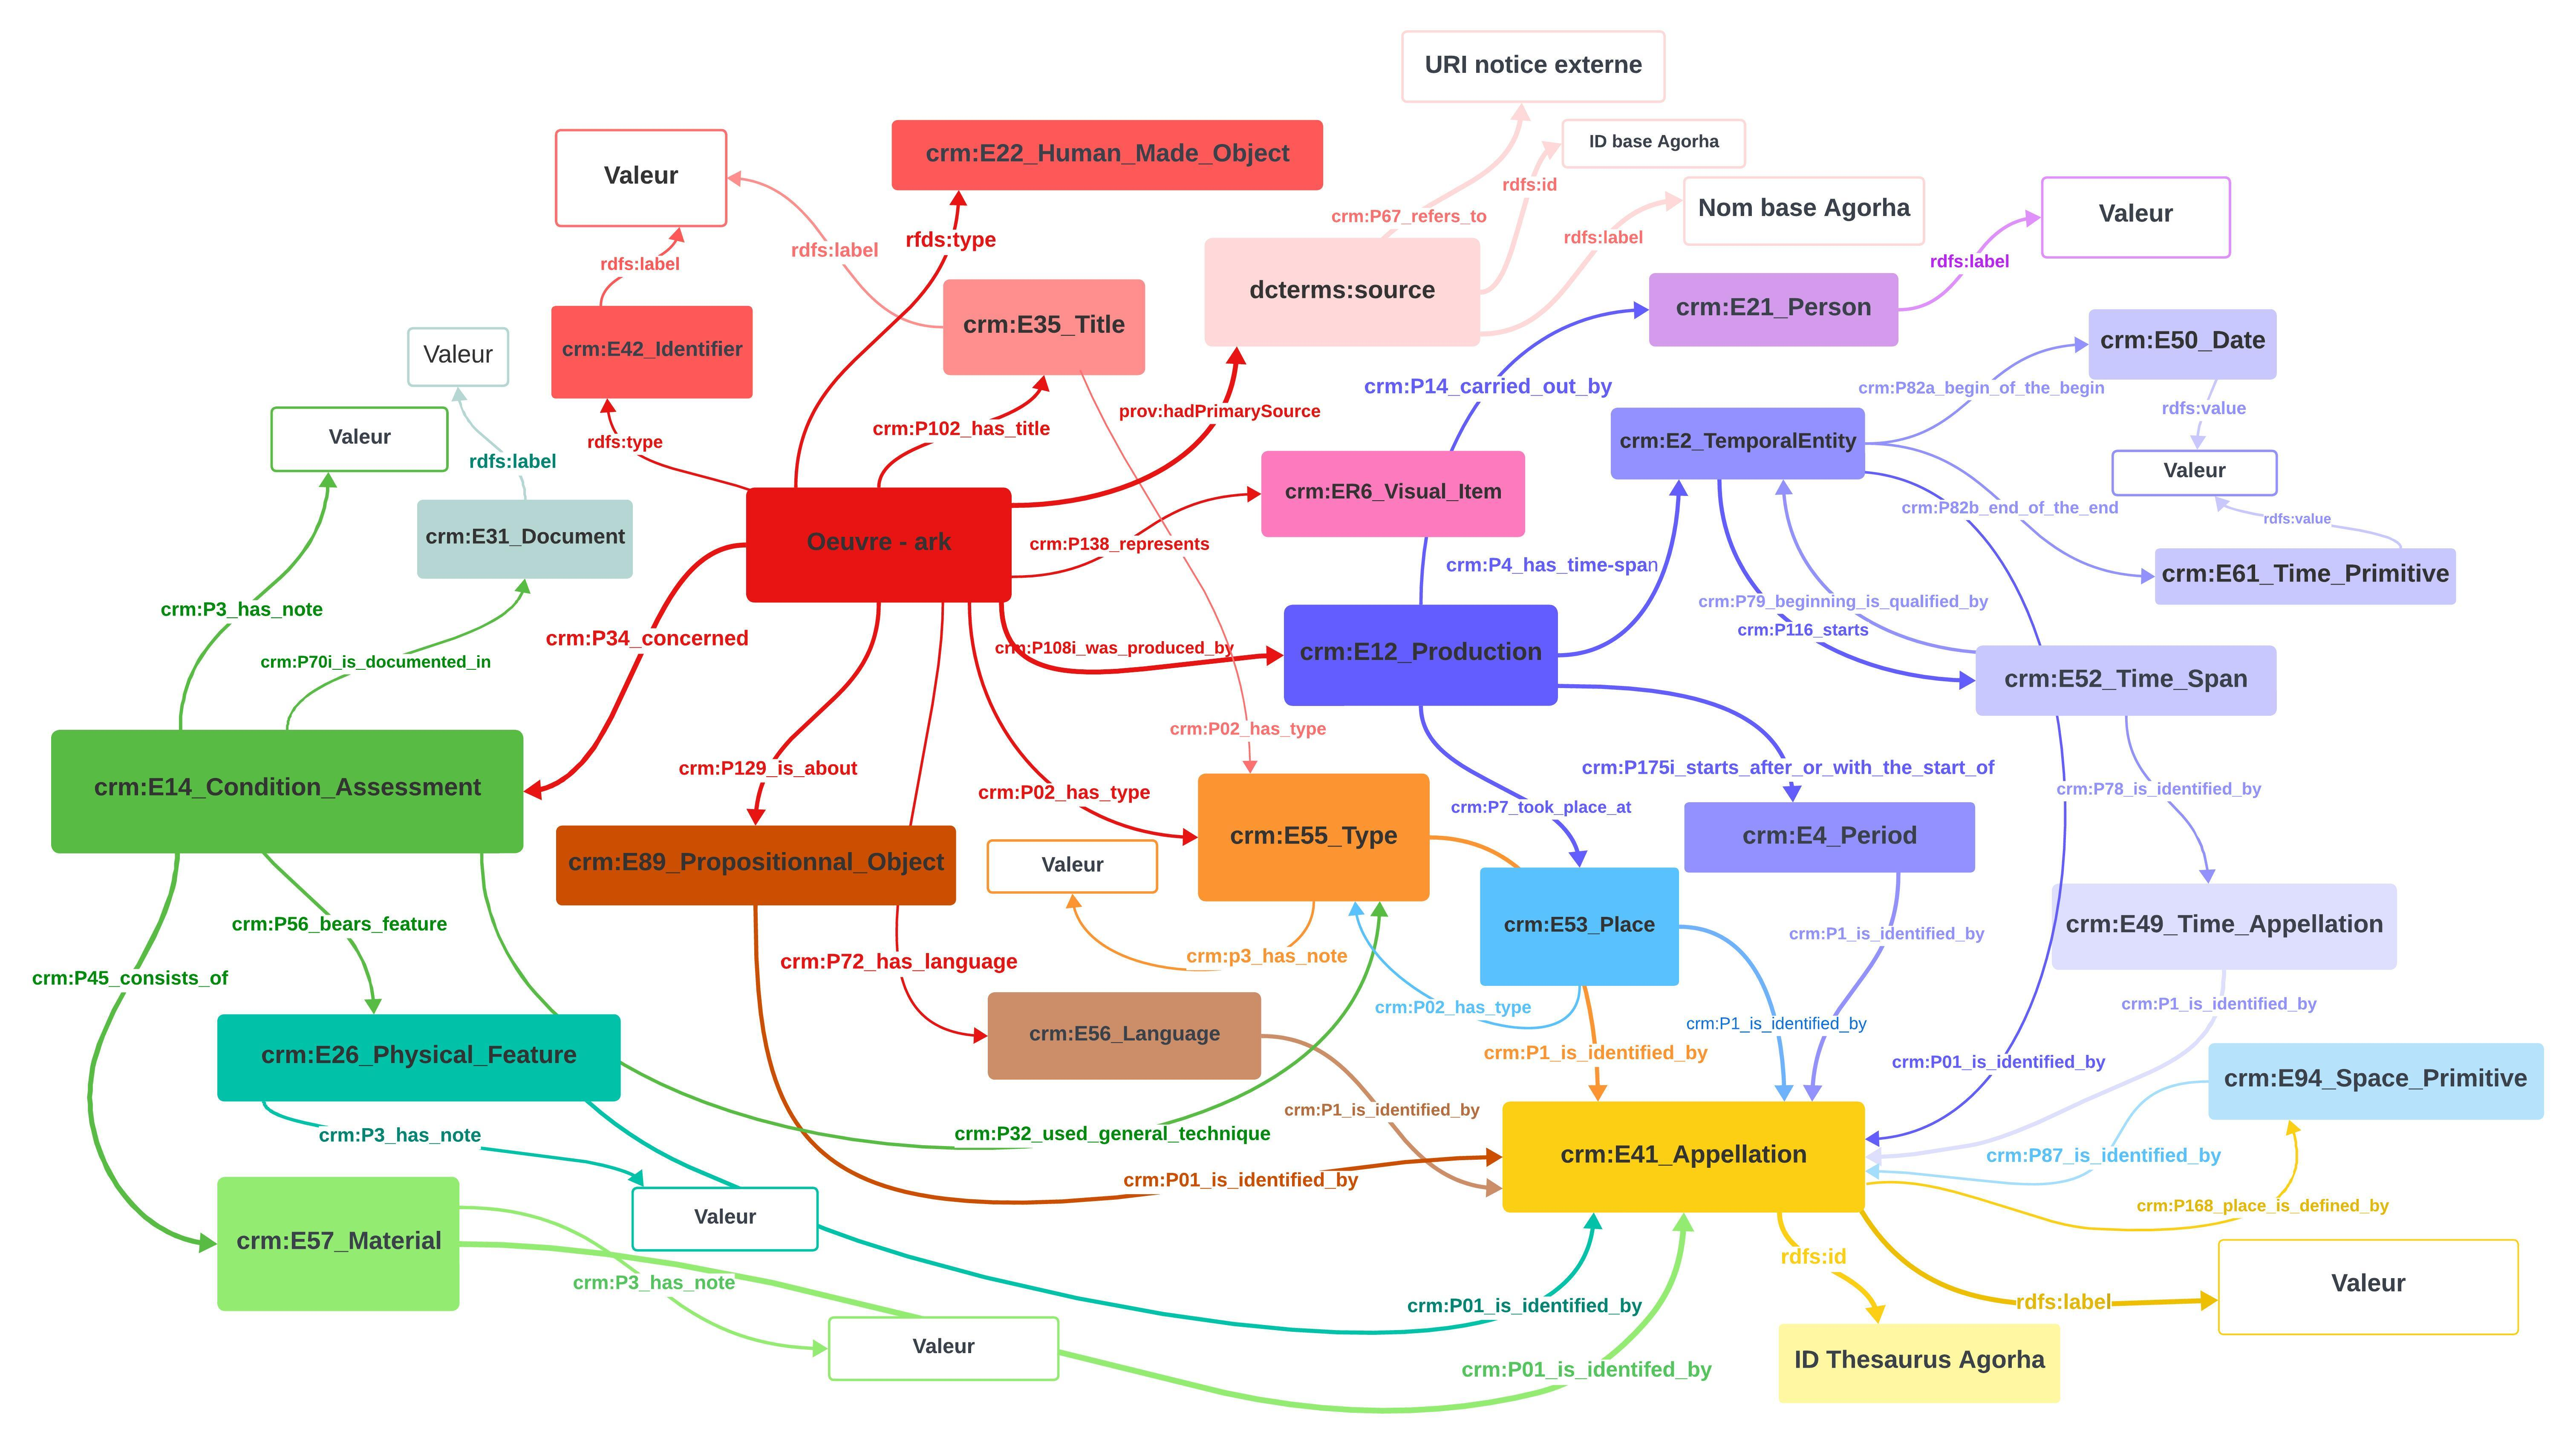
\includegraphics[height=9.43 cm]{images_memoire/modele_cidoc_agorha.jpeg}
    \caption*{\textbf{Organisation en entités-relations des données descriptives d'une notice Œuvre sur Agorha}\\
(Modélisation personnelle)}
    \label{Cidoc-CRM en pagaille.}
\end{figure}

Le format JSON, publié pour la première fois en 2003, vise à représenter une information par une simple paire clé-valeur, associées par deux points (:) à l’intérieur d’accolades (\{\}). Les paires clé-valeur peuvent être imbriquées les unes dans les autres pour reproduire directement leur hiérarchie sémantique. Une clé peut donc désigner indifféremment une chaîne de caractères, un chiffre, un booléen (une affirmation vrai/faux), un objet (une autre paire clé-valeur), voire un tableau (une série de paires clé-valeurs, ordonnées en liste). Un document JSON est donc une simple paire d’accolades contenant divers assemblages de clé-valeurs. Une notice JSON renseigne alors l’information \textit{type d’œuvre} ainsi~:

\begin{minted}[bgcolor=codetab, tabsize=2, fontsize=\small, xleftmargin=5pt, xrightmargin=5pt]{python}
{"content" : {#(contenu de la notice)
    "identificationInformation": {#(ensemble des informations identifiant l’œuvre) 
        "type" : {#(le type d’œuvre)
            "thesaurus" : [ {
            #(est un concept thésaurisé~: il peut #virtuellement en exister 
            #plusieurs, JSON inscrit donc une liste 
            #à cet emplacement.)
                "ref" : "https://thesaurus.inha.fr/thesaurus/resource/ark:/54721
                /2b45ed37-e436-439d-98b0-42d7a2434f4e",
                #(identifiant du concept)
                "prefLabels" : [ {#(terme priorisé)
                    "value" : "livre liturgique",   #(chaîne de caractères)
                    "language" : "fre"} ],#(langue)
                "conceptPath" : "/écrit/livre/livre religieux/livre liturgique"
                }]}}}} 
                #(résumé de la hiérarchie sémantique au #sein du thesaurus, 
                #et fermeture des #paires.)
\end{minted}

Le format JSON-LD (\emph{JSON for Linked Data}) est une extension du format JSON qui impose de qualifier sémantiquement les informations et leurs liens, en utilisant les schémas recommandés par le W3C, dont heureusement le CIDOC-CRM fait partie. Il est la transcription quasi-exacte de la construction par graphe montrée précédemment. L’information \textit{type d’œuvre} s’écrit donc ainsi~:

\begin{minted}[bgcolor=codetab, tabsize=2, fontsize=\small, xleftmargin=5pt, xrightmargin=5pt]{python}
{ #(cette Œuvre)
"crm:P2_has_type" : { #(a un type)
    "@type" : "crm:E55_Type",
    #(qui est un type précis, conceptualisé)
    "crm:P1_is_identified_by" : {
    #(qui est identifié par)
        "@id" : "https://thesaurus.inha.fr/thesaurus/resource/ark:/54721/79a9cacc-
        1ff8-495f-86b6-ae2dc9ad4401",
        #(un concept de thesaurus INHA)
        "@type" : "crm:E41_Appellation",
        #(qui est une ‘Appellation’)
        "rdfs:label" : {
        #(dont le terme est)
            "@language" : "fre",
            #(en langue française)
            "@value" : "peinture" }}}}
            #(cette valeur textuelle)
\end{minted}

Or dans les deux cas, les bases sont une simple accumulation de paires de clé-valeurs, toutes indépendantes~: l’ajout, la suppression ou la modification du contenu d’une paire n’a aucun effet sur les autres. Le contenu des bases peut donc être modifié à l’envi, sans devoir prendre en compte les contraintes structurelles des bases de données relationnelles. Même si le format JSON-LD impose d’utiliser des standards du Web pour renseigner le sens des données, et de les déclarer en préambule du document, il ne fixe pas le nombre de clés que ce dernier comportera, ni le nom qu’elles emploieront systématiquement, ni leur ordre d’apparition, ni combien de sous-informations imbriquées elles accepteront. Il s’agit donc de \textit{bases de données non-relationnelles}, également appelées \textit{bases NoSQL}, car leur absence de structure hiérarchique et relationnelle contraignante les rend impossibles à exploiter à partir de requêtes formulées en langage SQL (\emph{Structured Query Language}), mode opératoire le plus classique pour effectuer des extractions, modifications, ajouts ou suppressions d’informations ciblées. La structure des bases NoSQL est mouvante, ce qui facilite grandement la description d’objets intellectuels complexes, mais dont le détail n’est pas connu à l’avance. En effet, il arrive que les catalogues et rapports d’analyses physico-chimiques ne permettent pas de fournir l’entièreté des informations souhaitées. Les champs du tableur concernés resteront alors vierges, et il sera instruit au processeur de les négliger. Il sera toujours possible de modifier la notice par la suite~: l’interface graphique d’Agorha met tous les outils nécessaires en avant auprès des contributeur·ices. Mais pour les publics utilisateurs, une notice n’est pas une notice de catalogue. Car chacune propose une manière de comprendre un ensemble d’informations disparates, disponibles à un moment donné, sans que la conformité stricte des moindres léments de leur syntaxe à une norme internationale ne conditionne leur existence.

Les notices \textsf{Œuvre} des bases du projet Couleur gagnent en clarté en incluant les fichiers de numérisation des documents initiaux. Bien que ces numérisations aient été effectuées pour d’autres plate-formes (Gallica en tête), le service numérique de l’INHA les copie au préalable dans ses propres serveurs. Rappelons que certaines sont en effet modifiées pour marquer les zones de l’image analysées en laboratoire, et constituent alors des ressources documentaires inédites. Les fichiers de numérisation sont conservés sous trois résolutions~: \textsf{thumbnail} (miniature s’affichant à l’exploration des bases), \textsf{default} (image affichée au sein d’une notice en particulier) et \textsf{original} (fichier de haute qualité s’affichant lorsque les utilisateur·ices effectuent un zoom sur une zone). Le passage d’une résolution à une autre suit les fonctions des images à chaque étape de la navigation~; les dimensions sont fixées en adéquation avec le standard international IIIF, et renseignées au sein d’un document annexe nommé \textsf{Manifest}. La définition de ces catégories selon ces standards autorise l’ouverture des images numérisées au sein d’applications Web (qui autrement ne pourraient appliquer leurs modes opératoires automatisés), telles que Mirador\footnote{\url{https://projectmirador.org/}}, qui proposent des modes de visualisation enrichis (toute information souhaitée peut être intégrée librement dans un panneau latéral). Le SNR de l’INHA a expérimenté ces fonctionnalités sur le projet de recherche \textit{Digital Muret}\footnote{Par exemple, pour un collier aux perles sculptées, appréciable donc à plusieurs échelles~: \url{https://agorha.inha.fr/ark:/54721/735875e0-14df-412e-8b97-af22c13e61bf?database=73}}. Tout fichier image rattaché à un \textsf{Manifest} est affiché au sein de la notice avec les fonctionnalités de Mirador.

Les deux projets \textit{La fabrique matérielle du visuel. Panneaux peints en Méditerranée XIIIe-XVIe siècles} et \textit{La fabrique de l’art~: couleurs et matériaux de l’enluminure} hébergés sur Agorha sont donc le résultat d’une longue opération de création et d’éditorialisation des données documentaires et scientifiques. Même si leur contenu est encore fermé au grand public, ils constituent, pour quiconque détient des accès à Agorha comme contributeur·ice, des ressources potentiellement exploitables à des fins de recherche quantitative. Or la plate-forme, encore jeune – le lancement de sa version refondue, telle que décrite présentement, n’a pas deux ans – pose plus d’un paradoxe. Elle détaille les propriétés d’œuvres et de personnes du point de vue des événements qui les ont faites, et non de l’expérience qu’en ont par les publics. Elle élabore des thesaurus de termes à employer pour chaque information inscrite, sans toutefois aller jusqu’à imposer un nombre minimal et maximal de valeurs, ou le statut d’informations imbriquées, ou même un type de données incompressible (caractères libres, ou paramétrés en URI, nombres, dates...) Elle peut proposer des schémas intellectuels inédits~; et en contrepartie, le public ne peut que difficilement anticiper le contenu que chaque notice individuelle peut proposer.

\section*{1.3. Les impératifs contrariés du traitement automatique de l’information}
\addcontentsline{toc}{section}{1.3. Les impératifs contrariés du traitement automatique de l’information}

\subsection*{1.3.1. Les limites fonctionnelles d’Agorha~: une caractérisation de l’information inaboutie}

Le projet Couleur étant donc contraint par le temps, les différents stades de développement sont logiquement appelés à se superposer~; et le versement de notices dans Agorha commence alors que la définition des quatre thesaurus de description matérielle n’est pas achevée. Ce choix de passer au plus vite aux étapes suivantes du projet se justifie également par le besoin d’un espace de test~; ce que les contenus créés sur Agorha mais encore assignés au statut de \textit{« en cours de réalisation »} sont de fait.

Les quelques mille notices actuellement existantes dans Agorha (base INHA et base Manuscrits réunies) ont donc inscrit leurs données en utilisant le thesaurus obsolète \textsf{Matérialité}, dont la structuration sémantique est insatisfaisante sur trois points~:

\begin{itemize}
    \item Noms de couleurs, de matériaux et de techniques artistiques sont regroupés sans distinction\\
    
    \item Aucune propriété n’associe un matériau et ses possibles techniques de transformation (quand l’un va rarement sans l’autre, particulièrement pour l’usage de l’or)\\
    
    \item  Peu de matériaux sont répertoriés au sein de ce thesaurus, qui les répartit en quatre catégories (matières végétales, animales, minérales, synthétiques) dont les contours ne sont pas définis, ce qui suscite des interrogations quant au sort à réserver aux matériaux issus de la transformation artisanale de minéraux naturels (par cuisson, ou réactifs chimiques). Chaque catégorie comporte trois niveaux de spécification au maximum, ce qui peut paraître peu au regard du volume des taxonomies rédigées pour la géologie et la biologie.
\end{itemize}

Or les champs \textsf{Technique} et \textsf{Matériau} sont réservés aux affirmations dont les utilisateur·ices pourront ne pas douter~: ce qui se manifeste par l’emploi de termes thésaurisés. Dans l’attente de le publication de ces thesaurus, les informations concernées sont inscrites dans les champs \textsf{Commentaire}, afin qu’elles soient au moins disponibles pour être déplacées ou reformulées, sans nécessité de nouveau travail de lecture des documents-sources. Le temps manque pour autoriser un retour incessant sur les notices rédigées. En conséquence, des valeurs renseignant la même information (un nom de matériau ou de technique) se trouvent potentiellement dispersées au sein de plusieurs champs. Mais la réciproque est également valable. Peut-être du fait que le vocabulaire du CIDOC-CRM ait été jugé incomplet, ou que la décision de les intégrer aux notices ait été prise après les décisions concertées du comité scientifique, chaque \textsf{Commentaire} comporte des informations qui ne sont pas redondantes avec leur champ principal. Plusieurs données de signification différente sont localisées au même endroit. De plus, les champs \textsf{Commentaire} sont rédigés à la main (et non \textit{via} la sélection d’un terme proposé par menu déroulant), ce qui maximise le risque de disparités de saisie.

\begin{figure}[ht]
    \centering
    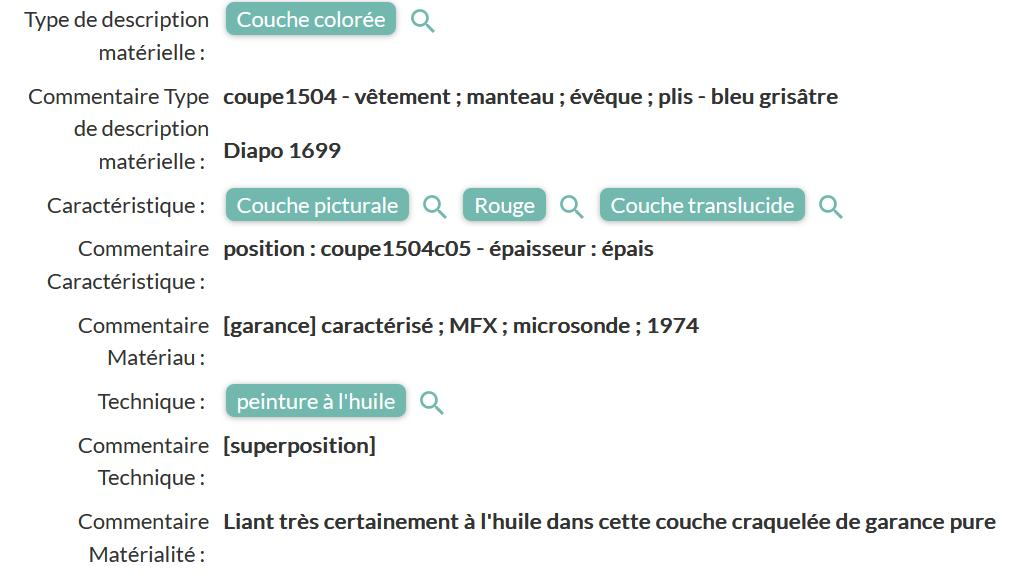
\includegraphics[height=9.33cm]{bloc_mat_standard.jpg}
    \caption*{Exemple d’un bloc \textsf{Matérialité} d’une notice de la base \textit{Panneaux peints en Méditerranée}, pour ici un total de 10 informations renseignées en texte simple dans un champ partagé,\\
    et 1 ensemble de renseignements non caractérisés en \textsf{Commentaire Matérialité}.\\
    (\url{https://agorha.inha.fr/ark:/54721/91dbb609-4789-4c7e-a7de-37c78f08d932?database=88})}
    \label{Un Bloc Matérialité normal.}
\end{figure}

Explorer les bases du projet Couleur à des fins herméneutiques requiert encore de croiser les données ensemble. Or l’actuelle configuration des notices ne permet pas de formuler des requêtes portant prioritairement sur le nom d’un motif et un matériau identifié, car ces informations, données en \textsf{Commentaire}, ne sont pas caractérisées par un identifiant ou un seul et unique emplacement. Car un moteur de recherche traite efficacement une requête à la condition que les informations demandées puissent être repérées automatiquement; elles doivent donc être marquées de manière unique, pour que la série d’instructions données au processeur le guident devant la bonne. Il sera alors nécessaire, tôt ou tard, d’éclater les champs en texte libre qui contiennent plusieurs informations, de n’employer que des termes issus de vocabulaires contrôlés, ou d’indiquer des liens logiques par l’usage de propriétés non ambiguës.

Car rien n’est trivial, pour un processeur. Il ne différencie pas les caractères d’un texte autrement que \textit{via} la reconnaissance de motifs qui lui ont été indiqués au préalable – tous ne sont que des séries de \textit{bits}. Un esprit humain, francophone et initié à l’histoire de l’art n’a aucun mal à déterminer le sens des informations notées en \textsf{Commentaire}, et comprendre les liens logiques, comme le fait que \textit{2021} à la fin d’un \textsf{Commentaire Matériau} désigne une date, et la date de l’analyse en laboratoire, non celle de la création de l’œuvre. Pour un processeur, ces informations, si elles sont sous la forme d’un texte libre, n’existent pas. De même, ce dernier ne considéra pas qu’une couleur verte, indiquée pour un motif, peut résulter de la superposition d’une couche bleue et d’une couche jaune. Il est nécessaire d’établir une syntaxe d’équivalences entre le concept de \textit{couleur verte}, caractérisé par son URI, et les concepts de \textit{couleur bleue} et \textit{couleur jaune}, en posant comme conditions que ces deux derniers se trouvent tous les deux associés au concept de \textit{mélange} au sein de leur bloc \textsf{Matérialité} respectif, et que ces blocs \textsf{Matérialité} détaillent la composition d’un même motif, caractérisé par son propre identifiant d’analyse.\footnote{Le calcul automatique de l’interaction des couleurs ne serait même pas vraiment envisageable si les couleurs étaient nommées par des valeurs chiffrées (telles que leurs proportions de Rouge, Vert et Bleu, et leur luminosité) elles sont créées par l’addition des rayons de lumières LED d’un ordinateur, quand la couleur des matières colorantes est due à la réflexion de la lumière naturelle une fois que les matériaux en ont absorbé une partie. Les calculs optiques ne seraient donc pas les mêmes.}

Plus préoccupante est l’absence d’instructions associées à l’utilisation de termes thésaurisés. Les décisions du groupe de travail scientifique insistent, à plusieurs reprises, sur l’importance d’attribuer un degré de certitude aux informations publiées. Toutefois, les voies empruntées s’avèrent inefficaces~: l’adjectif choisi pour qualifier l’identification d’un matériau, même s’il appartient à un vocabulaire contrôlé informel, se perd dans le reste du \textsf{Commentaire} où il figure~; un doute quant à une provenance, ou une technique, est également inscrite dans des \textsf{Commentaires}, en langage naturel (\textit{Syrie ou Turquie, reste à confirmer, (?)}). Il faudrait pouvoir lister au processeur tous les termes susceptibles de connoter l’incertitude, et lui instruire de vérifier leur éventuelle présence, pour que l’information soit prise en compte – tâche d’autant plus inenvisageable que les valeurs de certaines notices de la base INHA sont rédigées en anglais. Enfin, les estimations de dates de création disposent bien de termes thésaurisés pour indiquer un doute~: \textit{Avant, Après, Vers}. La documentation affirme que \textit{Vers} se traduit par l’ajout automatique d’une fourchette de 10 ans aux dates définies. Or aucune trace de cette opération ne se retrouve dans les données d’une notice téléchargée, quel qu’en soit le format. Les identifiants de ces termes dans leur thesaurus le sont, mais les chiffres correspondant aux dates sont strictement équivalents à ce que qui est affiché sur la page Web~: \textit{Vers 1490}, par exemple, reste \textit{1490-01-01 AD}. De même, pour \textit{Avant 1340}, la notice se contentera de donner la valeur \textit{1340-01-01 AD}, au mieux \textit{1339-12-31 AD}. L’information rendue, formellement identique à celle d’une date de création arrêtée, est donc faussée.

\subsection*{1.3.2. Les limites humaines à la démarche d’harmonisation}

Le projet Couleur est une démarche collective, menée par deux équipes de professionnel·les de deux institutions distinctes, visant l’élaboration d’un protocole inédit pour la représentation d’informations. Il va sans dire que la qualité du résultat est intimement corrélée à la qualité de la coordination de toutes ces personnes, et de la circulation des décisions prises d’un·e acteur·ice à un·e autre. Les expériences parfaites de ce genre sont rarissimes, sans même que la bonne volonté de chacun·e soit à remettre en cause~; l’ensemble des personnes impliquées dans le projet représente un domaine de spécialisation différent (histoire, chimie, science de la donnée, etc), et suivent des habitudes relevant de paradigmes méthodologiques variables. Le temps alloué au projet par chaque acteur·ice peut être également contrasté et mouvant en fonction des obligations inhérentes à chaque poste de chaque profession. Enfin, des perturbations extérieures telles que les confinements sanitaires, l’arrivée différée de contributeur·ices du fait de complications administratives, ou la défection de prestataires affectés à une tâche de développement précise impactent directement la circulation de l’information et la l’élaboration concertée du planning du projet. Dans ces conditions, certaines modifications de décisions préalablement actées ne sont pas connues de toute l’équipe, certaines prises d’initiative restent isolées, ou de simples malentendus persistent lors de la conception des notices. Les conséquences en sont aussi sournoises qu’implacables~: des pans entiers d’informations ne peuvent être exploitées par un processeur informatique.

Un exemple révélateur de ces paradigmes méthodologiques différant selon les spécialités, ainsi que de disparités résultant de changements réguliers des consignes de saisie, est le cas de la description des éléments d’une image – les motifs iconographiques – qui occupe le \textsf{Commentaire} du champ \textsf{Type de Description Matérielle} d’un bloc \textsf{Matérialité}.

\begin{figure}[!h]
    \centering
    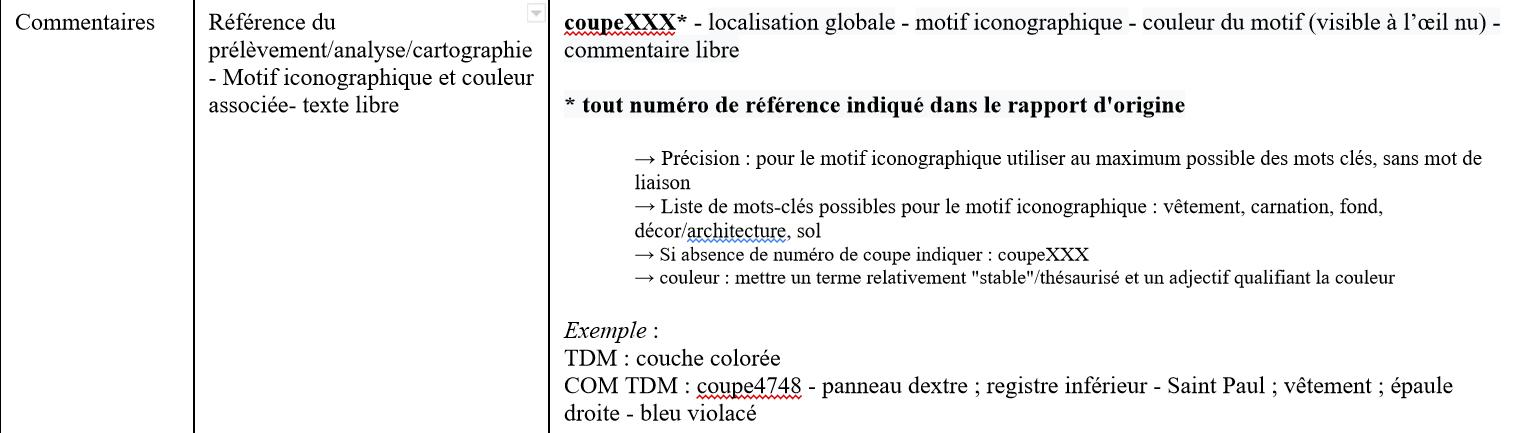
\includegraphics[height=4.79cm]{images_memoire/com_tdm_consigne_teresa.jpg}
    \caption*{Extrait du document \textit{Grammaire de saisie des COM MaJ7sept22.docx}, rédigé par le département des Manuscrits (Teresa \textsc{Knapowska})}
    \label{Consignes de saisie initiale}
\end{figure}

Ce document de consignes indique un ordre précis pour les informations du \textsf{Com TDM}~: \textit{identifiant, localisation, nom du motif, couleur} – séparées par un tiret. Chaque tiret vise à instruire au processeur que l’information inscrite a une autre signification que la précédente. C’est une manière de découper un \textsf{Commentaire} de texte libre en champs normalisés. Si le champ doit être multi-valué, les valeurs sont séparées par un autre signe de ponctuation (le point-virgule) pour que le processeur les traite comme telles.

\begin{figure}[!h]
    \centering
    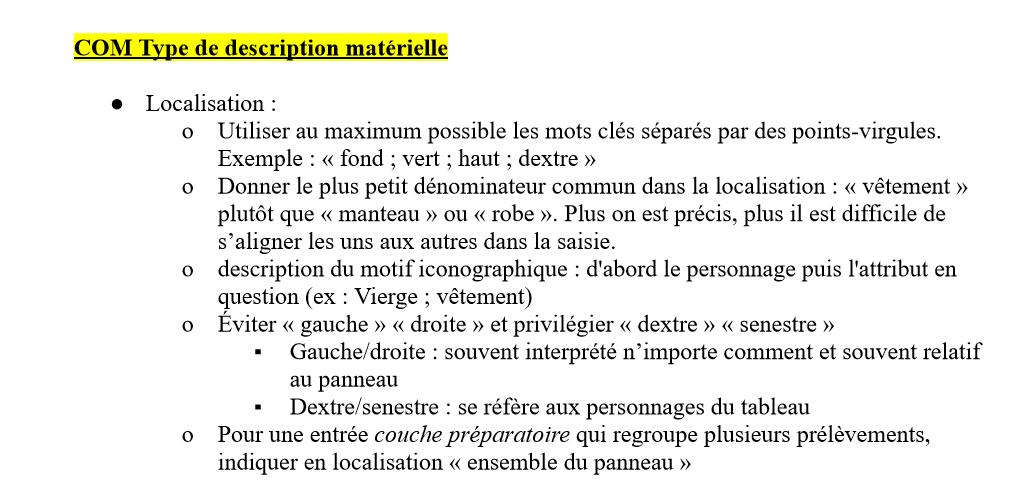
\includegraphics[height=8.17cm]{images_memoire/com_tdm_consigne_inha.jpg}
    \caption*{Extrait du document \textit{Writing rules AGORHA MaJ 7sept22.docx}, le premier visible dans le dossier partagé avec les contributeur·ices à Agorha, rédigé et utilisé par l'INHA.}
    \label{Consigne de saisie contradictoire}
\end{figure}

Or cet autre document de consignes indique les informations du \textsf{Com TDM} dans un ordre complètement différent~: que fait la mention d’une couleur parmi des termes relatifs à une localisation~? En réalité, le point de vue de l’INHA est qu’une couleur peut constituer une localisation -- après tout, c’est un élément visuel discriminant comme un autre. La localisation est aussi envisagée selon le point de vue du document, quand à de multiples reprises, les notices de la base Manuscrits prennent le point de vue du spectateur sur les images. Enfin, l’indexation des motifs semble également sujette à débat, puisque les consignes des Manuscrits privilégient la multiplication des termes (enrichissant ainsi la liste de concepts que le moteur de recherche reconnaîtra dans son répertoire) tandis que l’INHA priorise les plus génériques, susceptibles de renvoyer vers un maximum de documents. De plus, comme cela se retrouve dans cet exemple suivant, les mésusages des séparateurs sont fréquents au sein des deux bases~: marge supérieure senestre est indiqué en 3e position, avec ornement géométrique, ce qui l’assimile à un nom de motif iconographique. Cette disparité est due au fait que le contributeur, François Pacha Miran, qui est historien d’art, suit les consignes qui lui furent transmises par l’INHA.

\begin{figure}[!h]
    \centering
    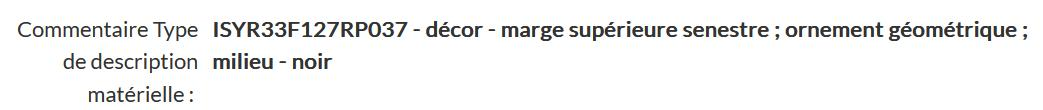
\includegraphics[height=1.78cm]{images_memoire/com_tdm_1_pachami.jpg}
    \caption{Notice: \url{https://agorha.inha.fr/ark:/54721/501a4925-5807-421f-9856-cbfcbe2ae0db?database=89}}
    \label{Un exemple de couac.}
\end{figure}

La syntaxe utilisée pour décrire l’emplacement de la zone analysée est d’autant plus ambiguë que l’INHA a d’abord considéré qu’une \textit{zone d’analyse} documentait une \textit{couche matérielle}, tandis qu’elle se rapportait à un \textit{motif iconographique} pour les Manuscrits. En effet les panneaux peints, à la différence de l’enluminure, sont conçus \textit{via} l’application successive de nombreuses couches de produits. Il est donc question de localiser une couche au sein d’une stratigraphie, car les couches n’y présentent pas les mêmes interactions. Elles peuvent être interdépendantes (au sein d’un mélange) ou non (les vernis ou couches préparatoires s’ajoutent à une peinture~; ils ne la constituent pas.) Mais les Manuscrits n’avaient même pas envisagé ce questionnement. Il fut décidé de ne pas réécrire les notices de la base Manuscrits existantes, et donc de ne pas établir de consigne collective pour la formalisation et l’emplacement de ce type d’information. Elle se retrouve donc aléatoirement en \textsf{Com TDM}, en \textsf{Com CAR}, en \textsf{Com Tech} (pour suppléer aux renseignements de type \textit{«~juxtaposition~»}). Si elle implique toujours une série d’identifiants de laboratoire spécifiques aux couches, ces derniers peuvent être introduits par un \textit{«~=~»}, un \textit{«~Voir~»}, ou ne pas l’être du tout. Au total, on ne sait pas trop où orienter le processeur, et pire, on ne sait pas trop vers \textit{quels termes}. Si aucun identifiant n’est renseigné, la caractérisation de l’information à rechercher va de fait poser des difficultés supplémentaires. On peut même partir du principe qu’elle n’est intégrée nulle part dans la base de données.

De ces disparités de saisie, qui s’ajoutent aux termes « mis en attente » avant la publication de leur thesaurus de référence, résulte un éparpillement manifeste de l’information~: comment assurer, alors, que le processeur saura systématiquement à quelle catégorie connue une valeur correspond~? Cette question est centrale à un traitement automatique.. Au printemps 2023, le SNR considère que le marqueur des informations inscrites en \textsf{Commentaires} est leur position au sein de celui-ci.

\begin{figure}[ht]
    \centering
        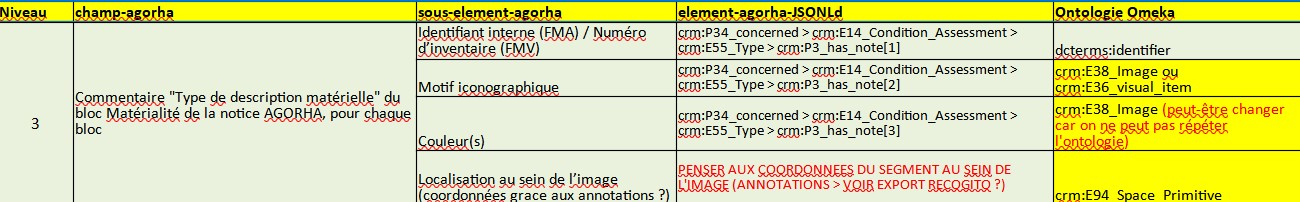
\includegraphics[height=2.64cm]{images_memoire/inha_mapping_motifs.jpg} 
        
   \smallskip
   
        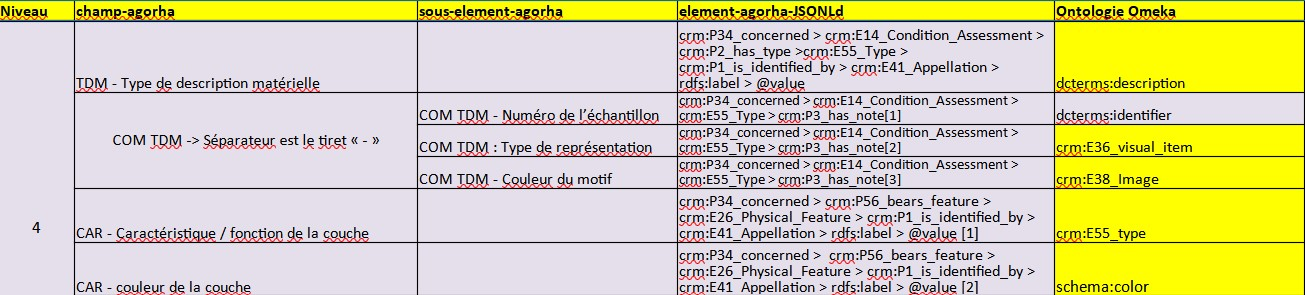
\includegraphics[height=3.80cm]{images_memoire/inha_mapping_couches.jpg}

    \caption*{Extraits du premier tableur de mapping Agorha-Omeka par le SNR (Chloé \textsc{Pochon}, Teresa \textsc{Knapowska}) Janvier 2023.\\
Cette opération sera détaillée en partie suivante.}
\label{fig:image2}
\end{figure}

On notera simplement la présence de chiffres entre crochets à la fin des emplacements JSON-LD, indiquent une position. Celle-ci est déterminée par l’usage de tirets, puis de points-virgules, et \textit{seulement ainsi}. Il en résulte que dans l’exemple suivant, qui ne montre pas de tiret, toutes les informations seront considérées comme les multiples valeurs du premier champ du \textsf{Com TDM}~: le numéro d’identifiant de l’analyse physico-chimique effectuée sur le motif.

\begin{figure}[!h]
    \centering
    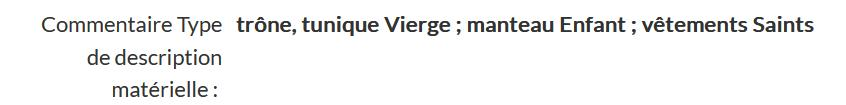
\includegraphics[height=1.85cm]{images_memoire/com_tdm_2_inha.jpg}
    \caption*{Notice: \url{https://agorha.inha.fr/ark:/54721/9251dae1-97ab-4613-b0a8-15606f194985?database=88}}
    \label{Un autre couac.}
\end{figure}

Un point plus préoccupant est l’absence d’identifiant d’analyse et d’emplacement du motif. Qu’elles ne soient pas disponibles est une chose~; que le reste des informations le soit ,et soit renseignées à la suite comme si de rien n’était, en est une autre. Car cela a pour effet de décaler la position de \textit{toutes} les informations qui succèdent à une information manquante~: sans numéro identifiant disponible, et sans localisation, le nom du motif se trouve en 1\textsuperscript{re} position, et sa couleur en 2\textsuperscript{e}. Le nom sera compris comme un identifiant, et la couleur comme une localisation. Chaque information non renseignée \textit{fausse} celles qui lui succèdent. Il est donc nécessaire de marquer l’absence d’une information, entre tirets, ou d’envisager un autre marqueur que celui de la position pour les informations des \textsf{Commentaires}.

Agorha peut se satisfaire des notices qui se présentent avec ces disparités grammaticales~: elles son destinée à une lecture directe par des chercheur·euses, ou à la des recherches en plein texte sur tout le contenu d’une notice ; elles ne pas d’emblée destinées à des fins de calcul statistique. Chaque notice atteint des niveaux d’informations très fins, mais qui n’ont pas tous besoin de marqueurs de champ et d’étiquettes thésaurisées pour être comprises par un esprit humain. Les notices publiées ainsi sur Agorha remplissent leur rôle documentaire vis-à-vis de leurs publics de chercheur·euses en sciences humaines. Ce sont les seules opérations de traitement automatique des données, pour un export groupé, ou des calculs statistiques en vue de la réalisation de graphiques portant sur l’ensemble de la base, qui requièrent une réécriture de l’information.

\subsection*{1.3.3. Des fonctionnalités de représentation graphique limitées}

Obtenir la représentation visuelle directe d’un phénomène constitue le Saint Graal des outils numériques d’aide à la recherche. Agorha propose donc ses services en la matière, accessibles par clic sur cette petite série d’icônes~: 
\includegraphics[height=0.4cm]{images_memoire/agorha_liens_dataviz.jpg}.
Tous ces services valorisent l’interaction directe avec les utilisateur·ices, et donc l’adéquation parfaite à leurs requêtes~: on obtient une variation de l’échelle d’information par mouvement de souris (amplitude spatiale et temporelle), et la mise en surbrillance des étiquettes au passage manuel du curseur – dont l’affichage demeure d’une pâleur assez illisible autrement.

Penchons-nous cependant sur le traitement des données, en prenant l’exemple de la base de l’INHA, qui a rendu 18 notices \textsf{Œuvres} publiques.

\begin{figure}[!h]
    \centering
    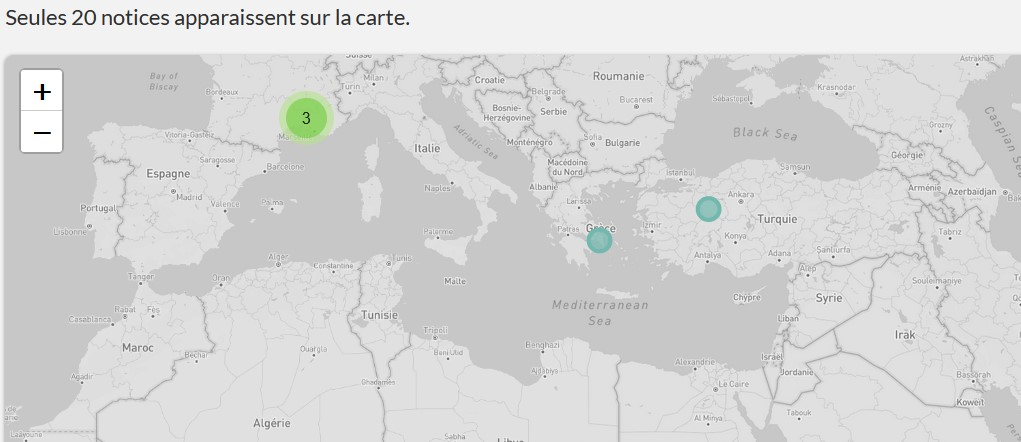
\includegraphics[height=7.36cm]{images_memoire/dataviz_carte.jpg}
    \label{Une cartographie faite par Agorha}
\end{figure}

La visualisation sur carte indique un unique lieu par notice~: il s’agit lieu de conservation de chaque œuvre, et non de son lieu de création, sans que nous en ayons décidé. Le fond de carte est invariablement un planisphère du XXI\textsuperscript{e} siècle, frontières et axes de circulation compris~; enfin, le nombre de notices traité ne correspond pas à celui indiqué dans l’onglet supérieur de la base.

\begin{figure}[!h]
    \centering
    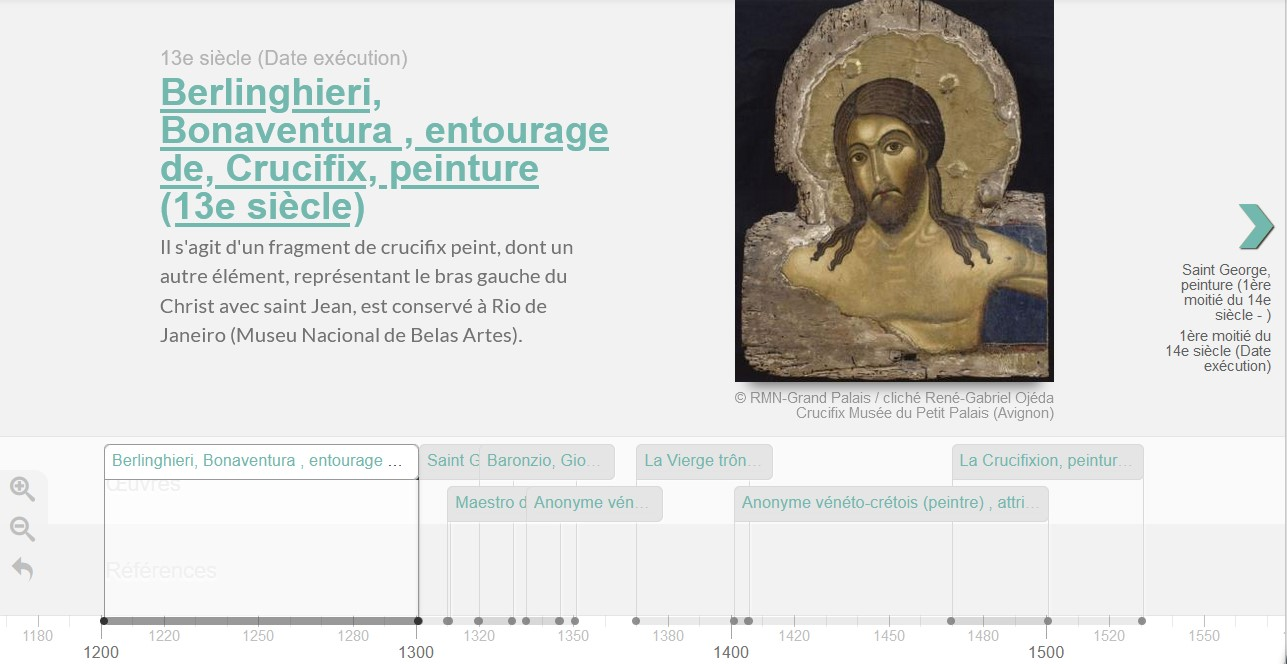
\includegraphics[height=8.77cm]{images_memoire/dataviz_chrono.jpg}
    \label{Une chronologie faite par Agorha}
\end{figure}

Les dates de segmentation de la visualisation par chronologie sont déterminées par défaut, à partir de la totalité des dates que la base a publiées. Il s’agit de dates de création d’œuvres, dont la seule association possible est avec leur titre, ce qui revient à n’obtenir qu’une chronologie de titres. La mention de personnes doit correspondre à des dates biographiques, mais il n’est pas précisé s’il s’agit de leur naissance ou de leur décès.

Ce mode de visualisation est à ne pas confondre avec les chronologies «~Dates début~» et «~Dates fin~», qui comptabilisent les titres parus par année, selon une date qui n’est pas directement identifiée (le début ou la fin d’une période de création~? D’une date d’analyse en laboratoire~?)

\begin{figure}[!h]
    \centering
    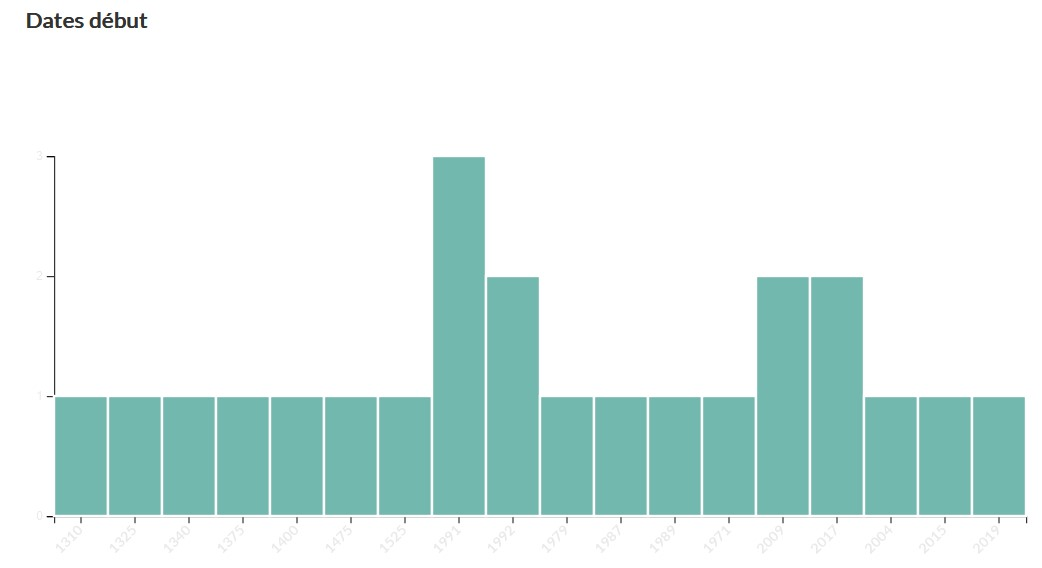
\includegraphics[height=9.27cm]{images_memoire/dataviz_graphiques_4.jpg}
    \label{Une autre chronologie par Agorha}
\end{figure}

Ce type de graphique, produisant des statistiques depuis quelques champs de notice choisis, se décline sur plusieurs modes.

\begin{figure}[!h]
    \centering
    \begin{subfigure}{}
        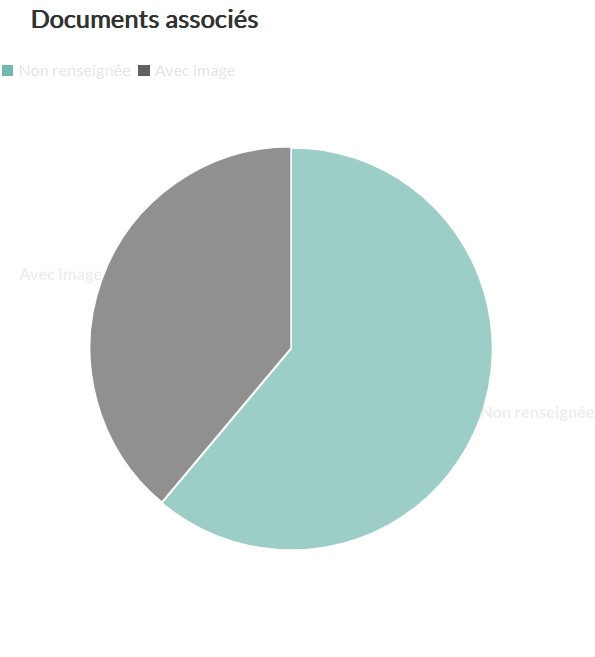
\includegraphics[width=6.22cm, height=6.90cm]{images_memoire/dataviz_graphiques_1.jpg} 
    \end{subfigure}
    \begin{subfigure}{}
        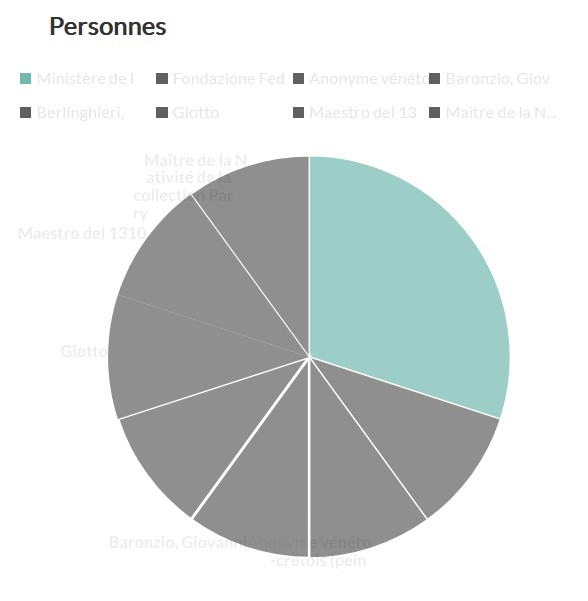
\includegraphics[width=7.31cm]{images_memoire/dataviz_graphiques_3.jpg}
    \end{subfigure}
\end{figure}

On trouve un aperçu des «~Documents associés~» dont la teneur est prédictible pour cette base, puisqu’elle se compose de notices \textsf{Œuvre} et \textsf{Référence} (dont les seuls médias liés sont les fichiers de numérisation des œuvres initiales), et qui présentement se heurte à la proportion de notices crées, mais non publiées au sein de la base (quelques 1500\% en juillet 2023) -- ainsi que la répartition des œuvres d’art par autorité, à la condition que cette dernière soit dotée d’une entrée dans le thesaurus Personne de l’INHA, afin de schématiser les écoles esthétiques dominantes.

\begin{figure}[!h]
    \centering
    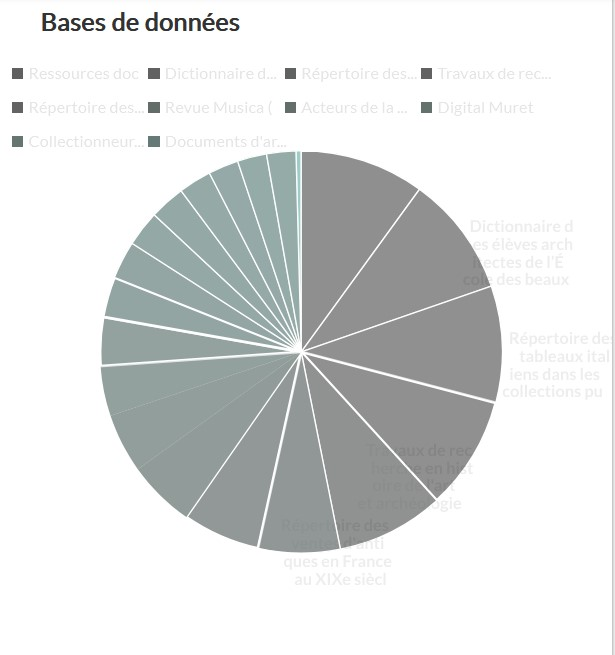
\includegraphics[width=8.81cm, height=9.4cm]{images_memoire/dataviz_graphiques_2.jpg}
\end{figure}

Il ressort de ces observations que les représentations graphiques fournies par Agorha ne sont pas conçues pour investiguer les problématiques propres à chaque projet de recherche~: les paramètres seraient autrement personnalisables par les utilisateur·ices, et proposeraient éventuellement d’interroger davantage de champs à la fois. Cela aurait toutefois pour conséquence de reléguer au second plan les potentiels liens intellectuels concevables avec les autres données publiées sur Agorha. Or c’est cette proximité rare entre des objets patrimoniaux si disparates qui constitue la richesse de la plate-forme, et son originalité dans l’éventail de ressources publiques dédiées à l’histoire de l’art sur le Web. Il est donc compréhensible que les représentations graphiques des données d’une base se focalisent sur des champs que l’essentiel des notices d’un même type partagent.

De ce fait, pour obtenir des représentations graphiques des données du projet Couleur conforme aux attentes initiales, et dans le temps dont le projet dispose, il sera nécessaire de développer \textit{en interne} les scripts adaptés. Ce dernier volet du projet commence par la conception d’un environnement numérique où ce travail sera déjà simplement envisageable~: deux nouvelles bases de données, dont les informations renseignées sont strictement les mêmes que dans Agorha, mais dont la structuration interne rend possible le traitement automatique. C’est en cela que consiste la définition d’une \textit{base d’exploitation}.

\clearemptydoublepage
\chapter*{2. Transformer les bases Agorha pour le traitement automatique}
\addcontentsline{toc}{chapter}{2. Transformer les bases Agorha pour le traitement automatique}

\section*{2.1. Mapping préliminaire : réorganiser l'information selon les paramètres d’Omeka S}
\addcontentsline{toc}{section}{2.1. Mapping préliminaire : réorganiser l'information selon les paramètres d’Omeka S}

\subsection*{2.1.1. Pourquoi initier une base d’exploitation sur un nouvel environnement~?}

On pourrait estimer que le perfectionnement des fonctionnalités existantes d’Agorha pour encourager la coercition des projets de recherche \textit{et} l’exploration des potentialités herméneutiques propres à chaque projet serait une opération plus simple à concevoir que l’architecture de nouvelles bases, doublée des protocoles de copie des données entrées dans Agorha. Or la question ne se pose pas à ce stade, car le SNR ne modifie pas ses modèles de fonctionnalités générales avant que l’efficacité et la robustesse des solutions envisagées n’aient pas au moins fait leurs preuves à l’échelle d’un seul projet. Proposer un exemple modeste mais pertinent d’utilisation de techniques computationnelles pour la représentation de problématiques scientifiques demeure la politique dominante. C’est donc une version prototypée focalisée sur les enjeux herméneutiques des bases du projet Couleur qui est attendue, dont la conception et les tests de lancement  ne doivent pas avoir d’incidence sur le fonctionnement présent d’Agorha.

Ce n’est pas une première pour le SNR, qui a déjà rencontré ce cas de figure pour le projet \textit{Digital Muret}. La procédure envisagée est la même~: recourir aux services du logiciel de configuration de bibliothèques numériques \textit{Omeka S} pour créer un nouvel espace de publication des données qui serait propre à leur traitement automatique. Omeka est un logiciel \textit{open source} développé depuis 2007 sur initiative du Roy Rosenweig Center for History and New Media, qui estimait l’offre en matière de sites Internet insuffisante pour la création des contenus image structurés par les standards de la documentation, particulièrement Dublin Core\footnote{Dublin Core, standard de description de contenus intellectuels fondé sur 15 éléments fondamentaux, est alors adoubé par la norme internationale ISO 15836 depuis novembre 2003 et porté par une vingtaine d’institutions de renommée mondiale, et en pleine phase d’adoption massive.}, au regard des perspectives qu’offrait le développement planétaire des blogs.\footnote{Source~: \url{https://omeka.org/about/project/}} Sa fonction est de réunir au sein d’un seul espace de travail tous les outils nécessaires à la création d’une bibliothèque numérique~:

\begin{itemize}
    \item Un outil de création de notices documentaires associant des fichiers image à des métadonnées Dublin Core, l’ensemble étant stocké dans une base de données relationnelle – des tables - hébergée sur le système des institutions. La gestion des données (ajout, suppression, modification,) est opérée de manière automatique hors de l’interface utilisateur, par des systèmes fondés sur le traditionnel langage SQL (\textit{MySQL, MariaDB, HeidiSQL}, etc). Seules les personnes en charge de la configuration initiale du logiciel au sein d’une institution ont besoin de connaître ces systèmes de gestion de bases de données~: la création de modèles de notices permet aux contributeur·ices d’interagir uniquement avec des formulaires exprimés en langage naturel. Chaque opération de création, suppression et modification des données s’opère par ces formulaires.

    \item Un outil de création de site Web pour l’affichage des notices, qui également traduit l’essentiel des contenus d’un document HTML en formulaires en langage naturel. Il permet au moins la personnalisation des onglets de navigation, de modes de recherche, de l’affichage des contenus à l’ouverture du site ou lors d’une recherche.

    \item La configuration de fonctionnalités précises est possible par le chargement de \textit{modules externes} spécifiquement dédiés et recensés sur le site d’Omeka~: il en existe de très variés, pour la gestion d’accès autorisés aux contenus, la création automatique de contenus depuis un import CSV externe, la visualisation ludique des fichiers image…
\end{itemize}

L’ensemble des fonctionnalités d’Omeka est écrit dans le langage de programmation PHP, extrêmement courant dès qu’il s’agit de créer des contenus Web appelés à interagir avec des utilisateur·ices externes, que ce soit par l’enregistrement d’utilisateur·ices ou \textit{via} de simples barres de recherche.

\begin{figure}[!h]
    \centering
    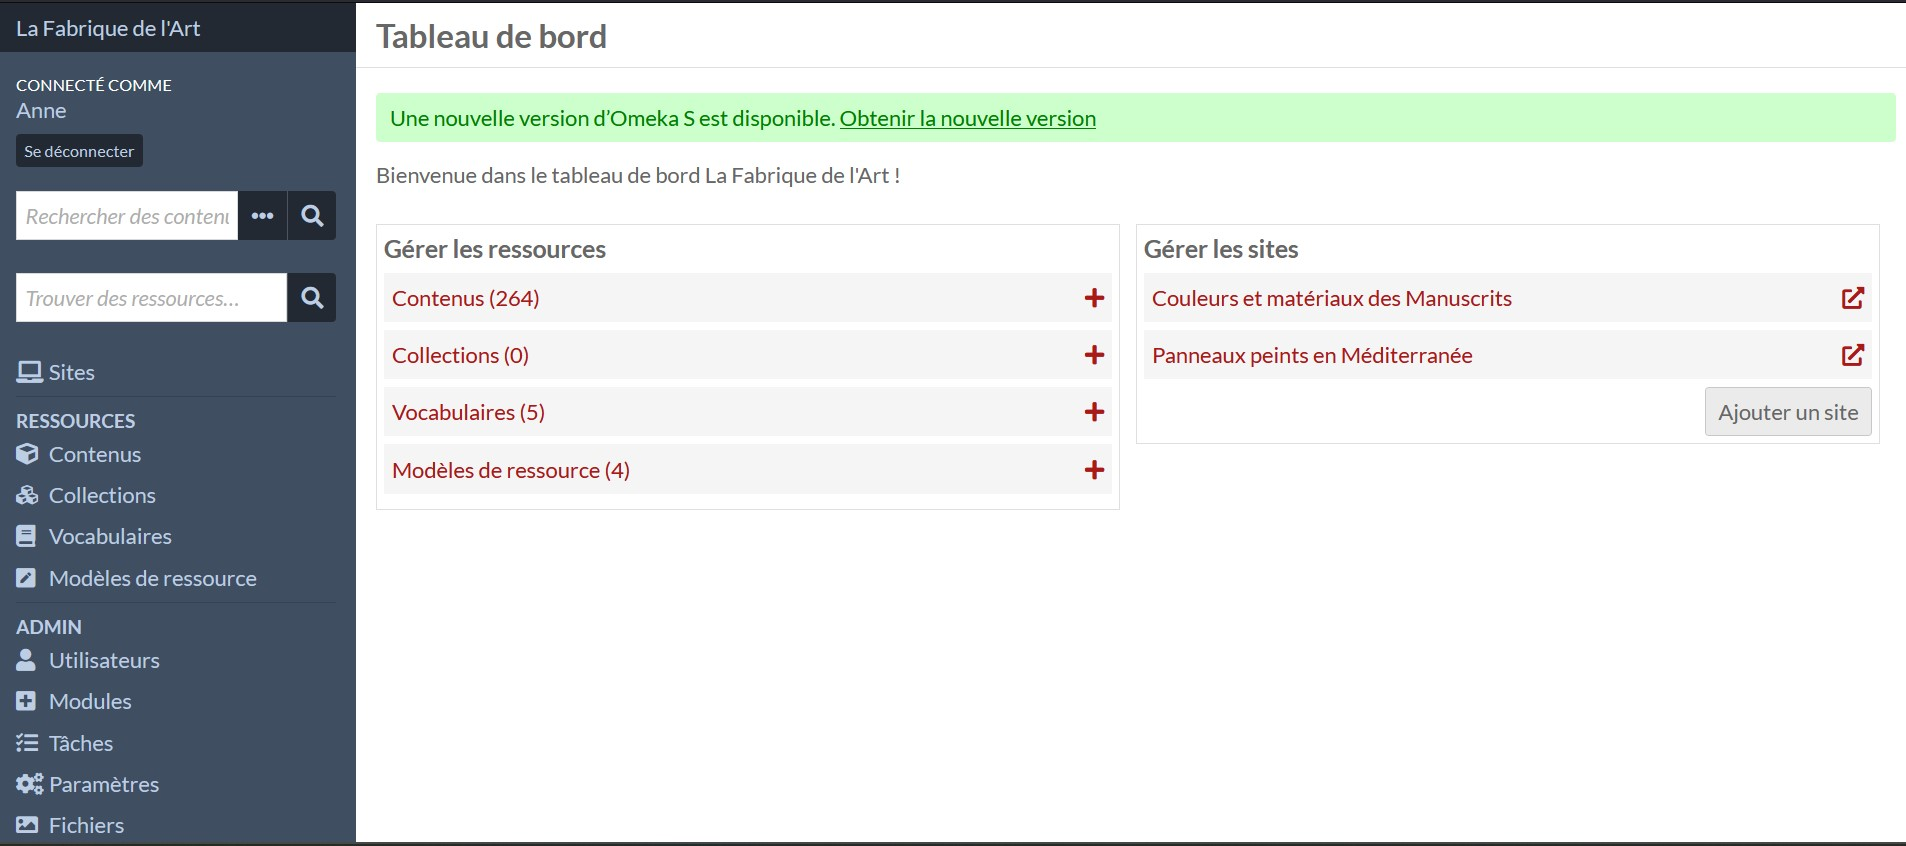
\includegraphics[height=7.46cm]{images_memoire/omekas_dashboard.jpg}
    \caption*{Aperçu de l’interface d’utilisation du logiciel Omeka S.}
    \label{Omeka S: Dashboard}
\end{figure}

Une notice, dans Omeka, peut virtuellement désigner bien des choses~; elles y portent donc le nom de \textit{Contenus}. Ces contenus peuvent constituer des ensembles nommés \textit{Collections}. Les fichiers externes liés aux Contenus ont, comme dans Agorha, le nom de \textit{Médias}.

L’objectif affirmé d’Omeka est que les institutions puissent créer facilement et rapidement (soit sans devoir nécessairement former l’intégralité de l’équipe contributrice aux requêtes SQL, à HTML ou à PHP) la ressource documentaire dont elles rêvent, sans contraindre  à l’hébergement et la maintenance de fichiers qui ne serviront pas, comme dans le cas d’autres logiciels similaires qui implémenteraient directement toutes les fonctionnalités possibles dans leur environnement. \textit{Omeka S}, choisi par le SNR,  est une version avancée du logiciel de base Omeka, dit désormais \textit{Omeka Classic}~; car il accepte la coexistence de multiples vocabulaires pour définir les propriétés d’une ressource – particulièrement s’il s’agit de ceux utilisés sur l’ensemble du Web, qui tendent à faciliter le partage et la réutilisation desdites ressources (\textit{Dublin Core, Schema.org, Bibo, CIDOC, IIIF}, etc.). Omeka S offre également davantage de modules externes, qui requièrent toutefois la compréhension du langage PHP pour être adaptés aux besoins spécifiques de chaque projet.

\subsection*{2.1.2. Formaliser la structure des notices à venir dans Omeka S~: le processus de \textit{mapping}}

Créer une base d’exploitation dans Omeka S nécessite donc d’y publier les informations existantes dans les bases Agorha du projet Couleur. Or copier l’architecture des notices Agorha telle quelle n’est pas pertinent pour Omeka~: la base d'exploitation enter compiler des données décrivant des \textit{choses}. On veut pouvoir associer des choses à d’autres choses~: des matériaux à des motifs, des motifs à des œuvres. Or nous avons vu que la plasticité d'Agorha était permise par l'usage du vocabulaire de référence CIDOC-CRM, qui décrit des événements. De plus, les liens sémantiques entre les valeurs entrées dans la base se comprennent par l’enchaînement de nombreux triplets d’information~; Omeka S n’accepte que 1 triplet pour renseigner une propriété d’un contenu donné. De plus, il n’est pas possible d’utiliser deux fois une le nom d’une propriété particulière deux fois~; si elle est sémantiquement acceptable deux fois, pour Omeka, c’est que les valeurs renseignent la même information. Or Agorha utilisait les mêmes propriétés pour renseigner la fonction d’une couche comme sa technique artistique employée. Si l’on veut associer 1 information à 1 propriété, il faut donc élargir les termes utilisés à d’autres vocabulaires de description de l’information sur le Web.

C’est l’établissement d’une table d’équivalence entre chaque information inscrite dans Agorha et chaque propriété créée pour Omeka S qui constitue l’opération dite de \textit{mapping}. Elle est détaillée dans son intégralité au sein du document tableur lié.

La base d’exploitation doit améliorer l’accessibilité des informations relatives à la matérialité des œuvres. Nous avons vu que celle-ci était compliquée par la syntaxe accumulative de blocs \textsf{Matérialité} au sein d’une même notice, qui les privait de leur singularité documentaire. Le SNR fait donc le choix de découper chaque notice Agorha en plusieurs notices Omeka, correspondant chacune à un niveau d’information donné. Cette définition des niveaux d’informations est initiée en janvier 2023, avant le début de ce stage. Elle commence par l’inventaire de \textit{toutes} les informations qu’une notice Agorha peut donner (ce qui donc ne correspond pas nécessairement au nombre de champs), et la sélection de celles à transmettre aux futures bases d’exploitation, qui sont les suivantes~:

\begin{quote}
    \textsf{Titre | Type d’oeuvre | Titre(s) alternatif(s) | Cote/n° inventaire | Lieu de conservation | Date de création | Lieu de création | Créateur(s) | Langue | Sujet général | Nom du motif iconographique | Localisation du motif iconographique dans l’image | Couleur du motif | ID d’analyse laboratoire du motif | Nature de la couche | Fonction de la couche | Technique picturale de la couche | Couleur de la couche | ID d’analyse laboratoire de la couche | Matériau | Degré de certitude de l’analyse | Observations annexes | Technique d’analyse laboratoire | Année d’analyse | Notices externes | Numérisation | Lien vers Niveau inférieur | Lien vers niveau supérieur}
\end{quote}

Nous pouvons également constater, à l’exploration des deux bases, la récurrence notable des informations suivantes~:

\begin{quote}
    \textsf{État de conservation | Restaurations opérées | Autres observations | Date de restauration | Éléments voisins | Épaisseur de la couche | Altération de la couche | Dimensions de la zone analysée}
\end{quote}

Elles ne s’intègrent non pas à l’ensemble de la contextualisation des conditions de création d’une œuvre, mais à l’ensemble de ses \textit{données de la conservation} mentionné dans notre première partie, et potentiellement cher au public des professionnel·les du patrimoine. Nous avons donc fait le choix de les intégrer aux notices Omeka, dans une démarche d’ouverture des publics potentiels des bases. La question de l’intégration d’autres informations encore – telles que les dimensions générales des œuvres, et leur historique d’acquisition – n’a pas été abordée.

Cerner les niveaux d’information, au sein de cette liste, revient à définir lesquelles peuvent constituer le cœur d’une recherche, et lesquelles y sont subordonnées. Quatre niveaux sont finalement arrêtés~:

\begin{itemize}
    \item \textsf{Œuvre}~: désigne l’ensemble documentaire d’une œuvre, tel que le corps d’ouvrage d’un manuscrit (l’ensemble de ses feuillets rassemblés en 1 unité physique, lacunes et rajouts compris) ou l’intégralité d’un polyptyque (fût-elle perdue.)

    \item \textsf{Image}~: désigne une unité picturale~: 1 panneau, 1 tableau, 1 feuillet d’un ouvrage.

    \item \textsf{Motif}~: désigne un élément visuel d’une Image présentant une unité de sens~: qu’il soit figuratif (personnages, créatures, plantes, bâtiments…) abstrait (fond uni, décor, ornements) ou une écriture (lettre, mot).

    \item \textsf{Couche matérielle}~: désigne un ensemble de matériaux appliqués dans un but précis (peindre un motif, préparer l’assiette d’une dorure, etc). Ce niveau correspond à la création d’un bloc \textsf{Matérialité} dans Agorha.
\end{itemize}    

Toutefois, les deux bases ne sont pas exactement d’accord sur le niveau où se situe la zone analysée (motif ou couche) La base Manuscrits considère que le la zone d’analyse représente l’ensemble d’un motif, par synecdoque. Sa localisation sera donc celle du motif. La base INHA considère parfois que la zone d’analyse est une entité en soi, dont on doit renseigner la localisation au sein du motif. C’est la raison pour laquelle le niveau d’information de la \textit{Zone analysée} a finalement été rejeté.

Puisqu’à 1 information devra correspondre 1 et unique propriété, certaines informations renseignées dans Agorha sont scindées. C’est d’abord du fait les données associées ne sont pas du même type, et n’appellent donc pas le même traitement automatique~: il n’est pas possible de cartographier un nom, puisque que la visualisation sur cartes s’opère au moyen de coordonnées \textit{chiffrées}.

\begin{itemize}
    \item \textsf{Lieu de conservation} devient alors \textsf{Lieu de conservation (nom), Lieu de conservation (coordonnées)}\\

    \item \textsf{Date de création} devient \textsf{Période de création (expression courante), Période de création (expression propre), Période de création (dates chronologiques)} – de fait, les datations étant fréquemment hypothétiques, c’est bien une période marquée par deux dates qui les qualifie.\\

    \item \textsf{Lieu de création} devient \textsf{Lieu de création (nom), Lieu de création (coordonnées)}\\
Une fois ces velléités de sémantisation supplémentaire des données engagées, le champ des possibles est vaste pour répondre à des besoins formulés par les publics scientifiques des bases à venir.\\

    \item Ainsi, la démarche de représentation des circulations de modèles esthétiques implique de différencier \textit{a minima} les rôles conférés à chaque créateur·ice, car ils n’entendent pas le même degré d’implication au sein du processus de création. Cette différenciation s’opère selon le terme thésaurisé employé sur Agorha dans le champ \textsf{Rôle}. Ainsi, l’information \textsf{Créateur} devient \textsf{Créateur, Contributeur, Inspirations}~; cette répartition de ces rôles en 3 catégories est personnelle, à des fins de test. Elle se présente comme suit~:\\

    \begin{itemize}
        \item \textsf{Créateur} regroupe \textsf{"de"}, (rapport direct d’autorité) \textsf{"collaboration", "associé à"}, (tous les acteur·ices sont à égalité dans le processus de création) \textsf{"attribué à", "anciennement attribué à"} (rapport direct également, bien que supposé)\\

        \item \textsf{Contributeur} regroupe \textsf{"achevé par", "commencé par", "copié par", "gravé par", "dessiné par", "peint par", "inventé par", "restauré par", "retouché par"} (chaque personne n’est responsable que d’une partie du processus de création, sans que l’on puisse assumer d’emblée qu’elle est à l’origine des choix esthétiques), \textsf{"atelier de"} (la responsabilité technique et esthétique est assumée par les chef·fes d’atelier), \textsf{"édité par"} (ne crée pas l’oeuvre, mais est responsable de sa mise à la connaissance du public)\\

        \item \textsf{Inspirations} regroupe \textsf{"cercle de", "école de", "entourage de", "lié à", "près de", "proche de", "suite de", "copié d'après", "d'après", "inspiré par", "genre de", "comparé à", "manière de"} (la personne associée n’a pas directement pris part ou supervisé le processus de création, mais reste une référence à mentionner pour comprendre l’œuvre).\\
    \end{itemize}

    \item \textsf{Couches matérielles} devient \textsf{Conditionnement | Support | Se compose de} selon la fonction de la couche.
\end{itemize}

Car tous les matériaux analysés ne figurent pas au sein d’un motif~: certains concernent le support du panneau ou du feuillet, ainsi que ses techniques de préparation, et se rapportent donc à l’ensemble de l’image (la notice correspondant à ces matériaux est donc qualifiée de \textsf{Support}, et renvoie vers une notice \textsf{Image}) Plus rarement, certains matériaux concernent le cadre d’un polyptyque, ou la reliure, ou couvrure, d’un manuscrit~; ils renvoient alors à l’ensemble d’une œuvre, et donc à une notice de type \textsf{Œuvre}.

C’est pourquoi les liens internes entre \textsf{Œuvre, Image} et \textsf{Motifs} ne sont pas les mêmes que ceux entre ces entités et les \textsf{Couches matérielles}. Déjà du fait que l’on s’exposerait au double emploi d’une même propriété (\textsf{dcterms:isPartOf}), mais aussi car l’idée visée n’est pas la même. On ne décrit plus ce qui est vu par les usager·es, ce qui constitue un propos, mais \textit{comment} ce qui est vu a été conçu, et de quoi il se compose physiquement. On choisira donc une autre propriété~: \textsf{crm:P106\_is\_composed\_of}, qui connote l’inclusion, mais aussi le rapport à la matière de l’élément, aussi prosaïquement que le terme \textsf{Composition} est employé pour renseigner la liste des ingrédients d’un produit alimentaire.

Les termes descriptifs peuvent également être variés selon le niveau d’information auquel ils se rapportent~: \textsf{Éléments voisins} devient ainsi \textsf{Image voisine} et \textsf{Motif voisin} pour les niveaux 2 et 3, \textsf{Couche inférieure du mélange, couche supérieure du mélange, autre couche indépendante} au niveau 4, sur demande de Sigrid \textsc{Mirabaud} pour la base INHA, dans le cas où l’on parviendrait à sémantiser la composition d’une stratigraphie. De fait, un public scientifique averti des caractéristiques de la production documentaire et artistique médiévale \textit{attend} de certaines propriétés de changer de valeur d’un niveau d’information à un autre~:

\begin{itemize}
    \item \textsf{Titre, Type d’oeuvre} et \textsf{Titre(s) alternatif(s)} changent du niveau \textsf{Œuvre} au niveau \textsf{Image}, car chaque \textsf{Image} d’un manuscrit comporte le numéro de son feuillet dans son titre.\\

    \item \textsf{Date de création, Lieu de création, Créateur(s)} et \textsf{Langue} changent également du niveau \textsf{Œuvre} au niveau \textsf{Image}, car il arrive aux chercheur·euses de croiser des feuillets ajoutés de manière postérieure à un ouvrage, et qui est donc susceptible de renseigner une provenance différente du reste.
\end{itemize}

À chaque niveau d’information va donc correspondre un type de notice~; et chaque type de notice renseigne ses données via un ensemble de propriétés – une par information.

Mais nous avons alors au total plus d’informations que nous avions de champs dans Agorha. De plus, les liens intellectuels y étaient renseignés par une série de triplets, à un degré d’information très fin~; or Omeka requiert la combinaison de 1 propriété (et une seule) et de sa valeur. Nous devons donc soit condenser un chemin intellectuel en 1 propriété, soit en déterminer une nouvelle. Mais à partir de quoi~? Nous aurions besoin d’au moins un nouveau schéma d’organisation des liens entre données pour le Web, de préférence un qui soit fréquemment utilisé. Choisir ensuite la bonne propriété reposera sur deux opérations~: Vérifier que l'on a bien compris 1. le sens de l'information scientifique dans Agorha et 2. le sens de la propriété standard choisie.

Les niveaux \textsf{Oeuvre} et \textsf{Image} partagent la quasi-totalité de leurs propriétés, puisqu’ils décrivent des informations documentaires~: la syntaxe CIDOC-CRM est donc simplifiée par l’emploi des termes familiers du standard Dublin Core. Toutefois Dublin Core seul ne suffit pas, car il ne propose pas de propriété pour se référer à \textit{l’objet intellectuel} dont sur lequel est centré la notice -- \textsf{Couches matérielles} et \textsf{Oeuvre} ayant peu en commun. On peut alors se tourner vers l’extension du standard Dublin Core, le \textit{Collection Type Vocabulary}, développé par le Dublin Core Collection Description Task Group en 2013 pour représenter une section dédiée aux sets d’objets de nature différente. Ce vocabulaire propose la propriété \textsf{cld:itemType}. La description officielle vise plus particulièrement le contenu intellectuel (\textit{The nature or genre of the content of one or more items within the collection.}) Mais d’un strict point de vue lexical, la mention du content n’apparaît pas~: \textit{item type} pourrait renvoyer simplement au \textit{type d’objet} en présence. Il existe bien une propriété \textsf{dcterms:type}, mais \textsf{cld:itemType} se montre plus précise en indiquant à quel niveau d’information elle se rapporte.

Nous devons aussi renseigner deux localisations~: celle du lieu de conservation, et celle du lieu de création. On ne peut donc pas utiliser deux fois \textsf{dcterms~:spatial}. La propriété \textsf{cld:isLocatedAt} peut remplir ce rôle, puisqu’elle fait explicitement référence au temps présent. Autrement, on cherchera des synonymes dans les autres standards~: \textsf{schema:locationCreated} fait explicitement référence au lieu de création~; et \textsf{schema:geo} est systématiquement associée à des coordonnées géographiques.

Une question similaire se pose pour renseigner la date de création. Certes, il n’y en aura pas des dizaines par objet. Or à chaque expression (\textit{4\textsuperscript{e} siècle – milieu du 6\textsuperscript{e} siècle}, par exemple) correspond son équivalent en chiffres, pour qu’il soit possible de générer des chronologies automatiquement. Il est important de les distinguer au moyen de propriétés différentes, pour indiquer à Omeka S de générer des chronologies sur celle des dates en chiffres seule. Car pour un ordinateur, dates comme chiffres correspondent à des numéros (encodage des caractères), et les valeurs textuelles figureront au sein de la chronologie en fonction des chiffres qui correspondent à leur premier caractère. Ce qui est indépendant, évidemment, de leur sens. Néanmoins, toute expression désignant une date est susceptible de correspondre à un terme entré en « recherche simple » par les utilisateur·ices. C’est pourquoi il nous faut plusieurs propriétés, pour que toutes figurent au sein de leurs notices, sans se confondre. On cherchera donc des propriétés synonymes au sein de vocabulaires différents~: \textsf{dcterms:temporal, dcterms:created} et \textsf{cld:dateItemsCreated}. Comme tous synonymes, ils comptent de légères variations~: le pluriel d’\textit{Items} (qui vise donc l’ensemble, non l’unité) et le terme de \textit{temporal}, qui vise explicitement une plage chronologique, non un point unique. Quasiment toutes les dates de création de nos notices sont effectivement des plages chronologiques~; mais la visualisation d’une chronologie préfère ne montrer qu’un seul marqueur. On attribuera donc \textsf{dcterms:created} aux dates en chiffres, destinées aux visualisations, et \textsf{dcterms:temporal} aux expressions nominales courantes. Certes, \textsf{dcterms:temporal} désigne également la période que le contenu intellectuel de l’œuvre décrit. Mais cette donnée ne figure pas dans Agorha.

Venons-en aux propriétés décrivant la matérialité de l’objet. C’est une préoccupation très lointaine au vocabulaire de Dublin Core, qui se focalise sur la mise en valeur des contenus intellectuels~; et on a vu que le modèle du Cidoc-CRM concevait ses notices comme un système d’événements. Les caractéristiques physiques d’un objet ne sont renseignées que par une ou deux propriétés (\textsf{crm:\_bears\_feature}), ce qui n’est pas suffisant pour la pluralité des points que les ressources \textsf{Couches matérielle} entendent détailler. Ceux qui, sur le Web, entend également détailler des caractéristiques physiques d’objets, sont les sites commerciaux. C’est le standard de Google \textit{schema.org}, adopté par les catalogues de vente, mais aussi les plate-formes de publications de revues spécialisées en tous genres, qui est le mieux équipé. Il se structure autour de 2 classes principales~: \textsf{Thing} (les choses, ce qui affirme la visée descriptive concrète du vocabulaire) et \textsf{DataTypes} (les valeurs non textuelles, ou les métadonnées descriptives précisant le type de valeur textuelle en présence.) \textsf{Thing} comporte 11 sous-classes thématiques principales, qui contiennent de multiples propriétés organisées en arborescence autour d’une notion conceptuelle. Ces propriétés ne sont toutefois pas exclusives aux notions qu’elles décrivent, et peuvent se retrouver à de multiples reprises. L’organisation en arborescence vise plutôt à faciliter la navigation de l’utilisateur·ice que de présenter des relations hiérarchiques closes. Les sections envisagées sont les suivantes~:

\begin{itemize}
    \item \textsf{CreativeWork (Thing>CreativeWork)}\\

    \begin{itemize}
        \item \textsf{schema:material} pour un matériau \textit{(A material that something is made from, e.g. leather, wool, cotton, paper.)}\\

        \item \textsf{schema:materialExtent} pour l’épaisseur d’une couche \textit{(The quantity of the materials being described or an expression of the physical space they occupy)}.\\

        \item \textsf{schema:position} pour la localisation du motif \textit{(The position of an item in a series or sequence of items)}, car parfois la localisation est le seul critère discriminant entre deux motifs très similaires.\\
    \end{itemize}

\item \textsf{VisualArtwork (Thing>CreativeWork>VisualArtwork)}\\

    \begin{itemize}
        \item \textsf{schema:artworkSurface} pour un conditionnement \textit{(The supporting materials for the artwork, e.g. Canvas, Paper, Wood, Board, etc)}\\

        \item \textsf{schema:artMedium}, pour une technique picturale \textit{(The material used. (E.g. Oil, Watercolour, Acrylic, Linoprint, Marble, Cyanotype, Digital, Lithograph, DryPoint, Intaglio, Pastel, Woodcut, Pencil, Mixed Media, etc.))} Bien que schema.org emploie le terme de matériau, ce sont plutôt des techniques qui sont décrites.\\
    \end{itemize}

\item \textsf{Product (Thing>Product)}\\

    \begin{itemize}
        \item \textsf{schema:color}~: pour une couleur \textit{(The color of the product)}\\

        \item \textsf{schema:hasMeasurement} pour les dimensions de la zone analysée \textit{(A product measurement, for example the inseam of pants, the wheel size of a bicycle, or the gauge of a screw. Usually an exact measurement, but can also be a range of measurements for adjustable products)}\\

        \item \textsf{schema:itemCondition} serait utilisé à la fois pour l’état de conservation d’une \textsf{Image}, et l’altération d’une \textsf{Couche}. \textit{(A predefined value from \textsf{OfferItemCondition}, specifying the condition of the product or service, or the products or services included in the offer. Also used for product return policies to specify the condition of products accepted for returns.)}\\

        \item \textsf{schema:isRelatedTo} pour l’ensemble des \textsf{Images} sœurs, \textsf{Motifs} frères et \textsf{Couches} se rapportant à un même objet \textit{(A pointer to another, somehow related product (or multiple products))} Nous pourrions envisager de montrer les autres occurrences d’un motif au sein d’autres Images via la propriété \textsf{schema:isSimilarTo}, \textit{(A pointer to another, functionally similar product (or multiple products))}, sans confondre avec \textsf{schema:isVariantOf}, qui pointe vers une entité abstraite commune à toutes les instances, non directement une autre instance.\\
    \end{itemize}

\item \textsf{Observation (Thing>Intangible>Observation)}\\

    \begin{itemize}
        \item \textsf{schema:measurementTechnique} serait utilisable pour la technique d’analyse physico-chimique \textit{(A technique, method or technology used in an \textsf{Observation}, corresponding to the method used for measuring the corresponding variable(s))}. On aurait pu utiliser \textsf{schema:usesDevice} \textit{(Device used to perform the test)}, de la catéogrie \textsf{MedicalTest}, si on avait voulu insister sur les aspects technologiques, mais il n’était pas question de livrer une étude comparative des appareils.\\

        \item \textsf{schema:observationDate} est retenu pour la date d’analyse \textit{(The observationDate of an Observation)}
    \end{itemize}
\end{itemize}

Renseigner le degré de certitude constitue le choix de propriété le plus difficile. On avait bien, dans la catégorie \textsf{Observation}, la propriété \textsf{schema:measurementQualifier} \textit{(Provides additional qualification to an observation)}, mais qui semble refuser de fonctionner avec des valeurs textuelles, au profit uniquement de numérables.

\begin{itemize}
    \item \textsf{schema~:interactivityType} de la catégorie \textsf{CreativeWork} \textit{(The predominant mode of learning supported by the learning resource. Acceptable values are 'active', 'expositive', or 'mixed')} au premier regard, ne correspond pas du tout~: elle décrit le mode d’interaction d’un public avec une œuvre d’art (\textit{active}, pour un jeu vidéo~; \textit{expositive}, lorsqu’il observe seulement~; \textit{mixed}, s’il observe, mais participe aussi à un degré mineur, comme lors d’un spectacle vivant?) Ce qui est dommage, car le sens lexical des termes anglophones pourrait bien représenter le fait qu’un·e chercheur·euse entretient bien un rapport d’interaction avec son discours, ou que le public lui-même doit veiller à son propre mode de réception des informations fournies.\\

    \item On peut envisager aussi \textsf{schema:status} \textit{(The status of the study (enumerated))} de la catégorie \textsf{MedicalCondition (Thing>MedicalEntity>MedicalCondition)} puisque cette propriété annonce un jugement porté sur une étude - si elle est \textit{achevée, en cours, reconnue,} etc. La même propriété se retrouve dans la catégorie \textsf{Event}, pour afficher si l’événement est passé, annulé, ou maintenu. Il s’agit donc d’une prise de parole des responsables au sujet de leur travail, ce qui peut correspondre à l’énonciation de degrés de certitude relatifs à l’identification des matériaux d’une couche.
\end{itemize}

Pour les informations renvoyant à la qualification des liens logiques et scientifiques, nous pouvons envisager un retour au vocabulaire CIDOC-CRM, en n’acceptant qu’une seule propriété pour chaque~:

\begin{itemize}
    \item \textsf{crm:P15\_was\_influenced\_by} pour la désignation des \textsf{Inspirations}~;\\

    \item \textsf{crm:P106\_is\_composed\_of} et son inverse~: \textsf{crm:P106i\_forms\_part\_of} pour la composition matérielle d’un motif ou d’un support~;\\

    \item \textsf{crm:P134\_continued} (pour indiquer la prolongation d’un processus partagé, ce qui peut désigner une autre Couche participant à un mélange)\\

    \item \textsf{crm:P31i\_was\_modified\_by} (parce qu’un objet se trouve modifié par l’opération de restauration qui a été effectuée) (propriété inversée)
\end{itemize}

L’ensemble de ces propriétés déterminées pour chaque niveau d’information constitue le modèle de chaque type de notice envisagé pour les bases d’exploitation. Omeka S propose de les stocker en tant que Modèles de ressource, pour que chaque \textsf{Contenu} créé à la main sur la plate-forme offre d’emblée quatre modèles de formulaires possibles.

\begin{figure}[!h]
    \centering
    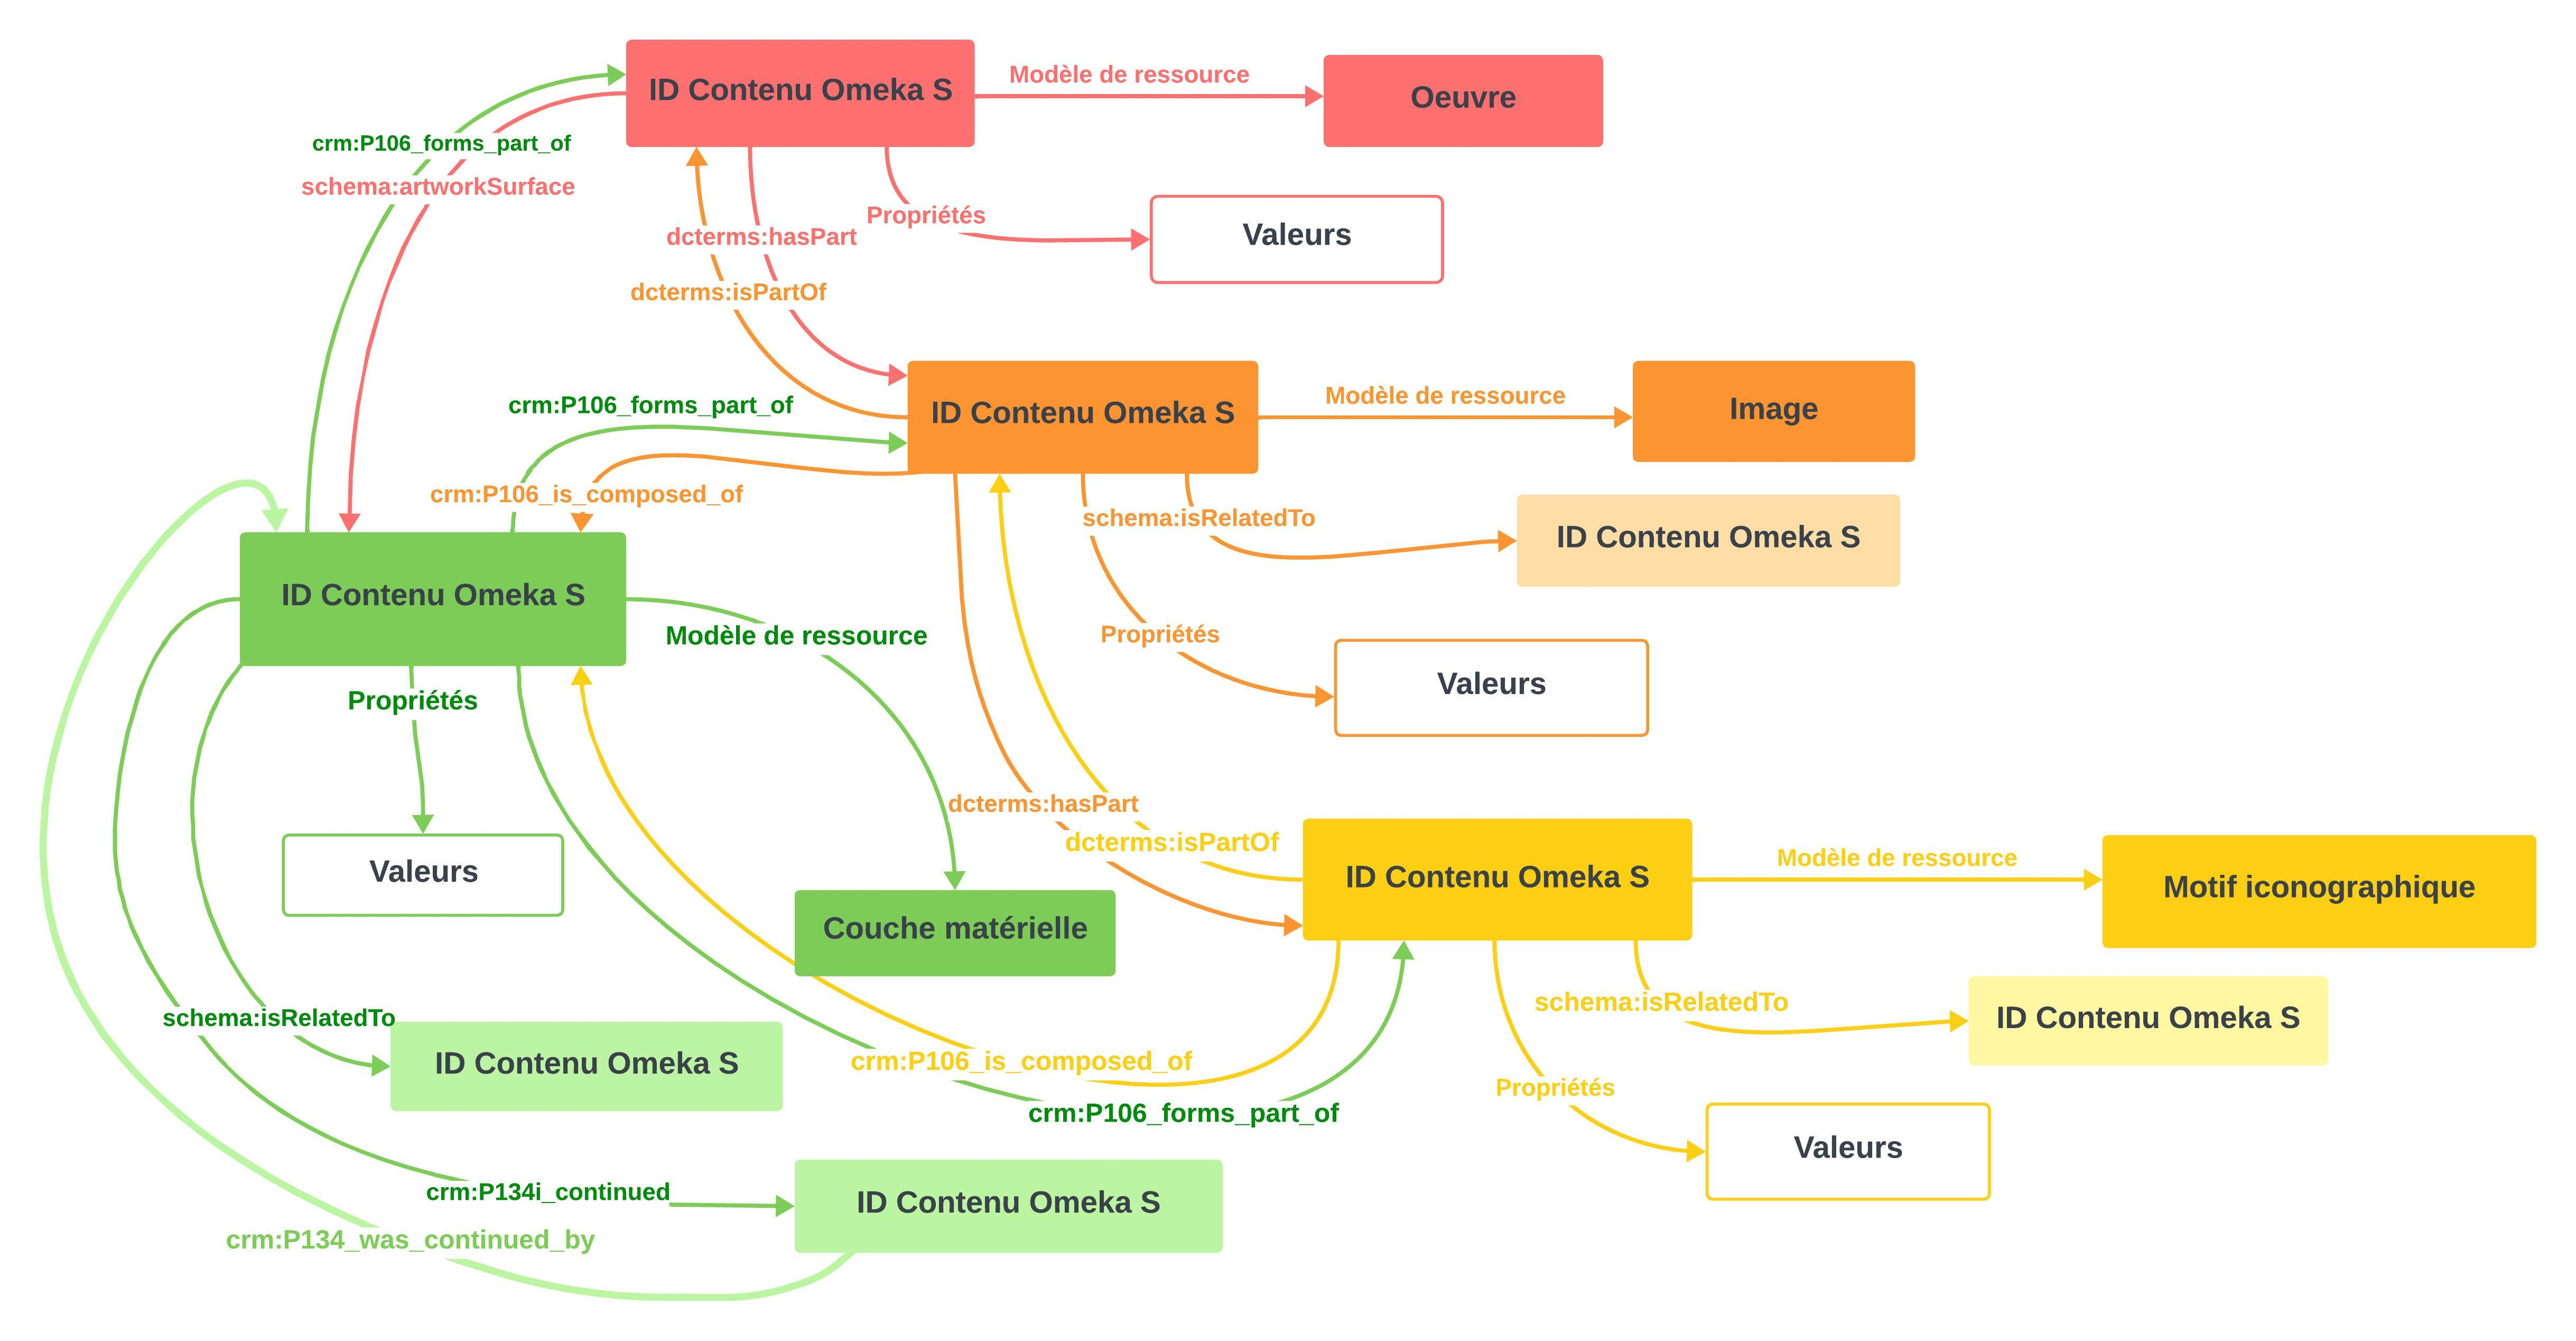
\includegraphics[height=8.74cm]{uml_omeka_s.jpeg}
    \caption*{\textbf{Organisation de l'information dans Omeka S~: l'interaction des 4 modèles de notice}
(Modélisation personnelle)}
    \label{Schématisation de l'information pour Omeka S}
\end{figure}

\pagebreak

\section*{2.2. Constituer le contenu d’une base pour Omeka S}
\addcontentsline{toc}{section}{2.2. Constituer le contenu d’une base pour Omeka S}

L’INHA est une structure collaborative de chercheurs~: ce qui signifie que de multiples personnes travaillent simultanément sur un même projet, et qu’il est nécessaire de réunir leurs contributions à un même endroit. Agorha offre la possibilité de verser des données depuis n’importe quelle connexion Internet, et un compte avec les droits de contributeur·ice~; c’est là une procédure autrement plus simple que la connexion par SSH\footnote{\emph{SSH}, pour \emph{Secure SHell}, est une procédure de connexion à un serveur central via un canal sécurisé, comme – l’intranet d’une institution – qui requiert donc la configuration d’un réseau privé, et d’une session pour chaque contributeur·ice, accessible depuis ce seul réseau privé (comme l’intranet d’une institution). Or les simples contributeur·ices à Agorha, mais externes au SNR, n’ont pas à avoir accès aux dossiers de travail du projet, ni à ceux de la configuration logicielle.} à l’ordinateur central qui héberge les données.

Il en résulte que l’ensemble des données créées jusqu’à ce jour ne se trouve que sur ledit ordinateur central. Pour les transférer en vue de la création des bases d’exploitation, il sera donc nécessaire de les récupérer depuis Agorha elle-même, par requête Internet.

\subsection*{2.2.1. Décision de consignes de nettoyage des données}

Encore faut-il que les données publiées sur Agorha soient exploitables telles quelles~: on ne peut s’abstraire de l’étape de la correction des disparités remarquées, dite \textit{nettoyage des données}. Elle se traduit par la mise à jour de tous les documents de consignes de saisie, afin que les contributeur·ices assurent les modifications eux-mêmes. L’objectif est de désambiguïser les informations inscrites dans les \textsf{Commentaires}. Le SNR fait le choix de ne pas indiquer l’absence d’une information, qui nuirait au confort de lecture, en utilisant le terme consacré en langage SQL pour tout champ vide~: la valeur \textit{\textsf{NULL}}. Il est donc conclu à la place d’apposer systématiquement une étiquette devant chaque type d’information, qui renseigne sa signification (et contribue ainsi à améliorer encore la lisibilité des blocs \textsf{Matérialité} pour des yeux humains). \textit{\textsf{identifiant~:, localisation~:~, motif~:~, couleur~:~}} pour le \textsf{Commentaire de Type de Description Matérielle}~; \textit{position~:~, couleur~:~, épaisseur~:, altération~:~} pour le \textsf{Commentaire Caractéristique} (avec la demande que toute information annexe soit séparée par un tiret)~; \textit{\textsf{matériau~:~, certitude~:~, technique~:~, dimension~:, date~:}} pour le \textsf{Commentaire Matériau}. Bien que le champ reste rempli en texte libre, seuls ces termes sont autorisés~: car il devient possible de les caractériser auprès des processeurs, au moyen de \textit{regex}\footnote{Une \emph{regex}, ou \emph{expression régulière (REgular EXpression)} est une séquence de caractères spéciaux utilisée pour cibler et manipuler une fraction choisie d’une chaîne de caractères.}. L’information peut alors être extraite quelle que soit sa position dans le champ de \textsf{Commentaire}.

Les \textsf{Commentaires Matériau} et \textsf{Technique} voient également leur séparateur de champ être redéfini. Le \textsf{Commentaire Technique} comporte en effet tout terme en attente d’être thésaurisé (ce qui se traduit, sur Agorha, par son inscription [entre crochets])~; mais un certain nombre d’observations diverses, en texte libre, peuvent aussi y figurer. Les séparer par un tiret permet d’instruire au processeur de les négliger~; en contrepartie, si plusieurs termes en attente de thésaurisation figurent, ils devront employer le séparateur de second niveau, soit le point-virgule. (Les virgules ne sont pas rares à cet emplacement, mais c’est une option supplémentaire minime à indiquer au processeur.) Le \textsf{Commentaire Matériau} obéit à une structuration plus complexe. Les informations \textit{\textsf{matériau~:~, certitude~:~, technique~:~, dimension~:~, date~:~}} n’y sont pas des champs, mais des sous-champs~; car plusieurs campagnes d’analyses ont pu être réalisées identifier les composantes d’un même produit. Il est souhaitable de les séparer, pour que chaque résultat d’analyse puisse être contextualisé – autrement, les informations \textit{\textsf{matériau~:~, certitude~:~, technique~:~, dimension~:~, date~:}} compteront plusieurs valeurs, sans qu’il soit \textit{a priori} possible de savoir à quelle campagne d’analyses elles se rattachent.\footnote{Problème qui n’a pas (encore) été résolu pour le modèle de ressource \textsf{Couche matérielle} dans Omeka S~: les informations de deux, voire trois campagnes d’analyses relèvent des mêmes propriétés sémantiques, et les valeurs associées se trouvent toutes regroupées, en perdant leur contextualisation.} Il est donc prescrit de renseigner les campagnes d’analyses les unes après les autres, séparées par un tiret~; or ces cas sont encore rares à l’échelle des bases de données du projet Couleur, d’où le caractère contre-intuitif de cette consigne pour les contributeur·ices. Néanmoins, toute rare qu’elle soit, cette information permet d’associer l’occurrence d’un matériau à un nombre d’analyses~; plus elle est documentée, plus les marges d’erreur et d’hypothèses se réduisent. On peut donc, en comptant cette information, élaborer un système de quantification du degré de certitude de l’identification d’un matériau. À terme, il inclurait également la prise en compte l’ensemble des informations du \textsf{Commentaire Matériau}, en attribuant un coefficient aux quatre valeurs possibles de l’information \textit{\textsf{certitude}}, ainsi qu’à la dimension de la zone analysée (car plus une zone d’analyse est restreinte, plus son information est fiable) et à chaque technique d’analyse employée (sur conseils à solliciter auprès des professionnel·les du patrimoine.)

Savoir si les corrections des notices peuvent être automatisées est sujet à débat~; le SNR envisage la modification des tableurs initialement utilisés par les contributeur·ices pour inscrire les données des rapports d’analyse, et d’effectuer un nouvel export massif de ces tableurs dans Agorha. Mais apposer une étiquette à une information requiert de connaître son sens, particulièrement dans le cas où leur ordre au sein des \textsf{Commentaires} n’est pas fixe, ce qui nous ramène à notre problème actuel, traité en partie \emph{1.3}. La correction de quelques 200 notices au cours du mois de juillet 2023 a été faite à la main, dans le but de fournir des données de test au script d’extraction des informations. Car autrement, trop de temps serait consacré à déterminer si les erreurs rencontrées proviennent de défauts d’écriture du script, ou de la configuration initiale des bases sur Agorha.

\subsection*{2.2.2. Extraire les informations des notices Agorha par script automatique}

La première étape évidente est de télécharger l’ensemble des notices de type \textsf{Œuvre} de chaque base (une fois corrigées, cela s’entend). Leur volumétrie excluant d’ouvrir et télécharger chaque notice individuellement, on peut utiliser les services d’une API\footnote{Une \emph{API, Application Programming Interface}, est est un ensemble de protocoles établis pour permettre à différentes applications informatiques d’échanger des données entre elles de manière harmonisée. Les règles syntaxiques de la requête utilisée par le SNR signifient littéralement~:\textit{«~Nous souhaitons parcourir les notices pour exporter leurs fichiers JSON, si elles en possèdent~; plus particulièrement, parcourir les notices de type \textsf{ARTWORK} de la base 89.~»}} à cette fin. Or si Agorha autorise effectivement le téléchargement des notices d’une table, toutes concaténées au sein d’un seul fichier, aucune interface publique pour le traitement de requêtes n’existe encore. Il est donc nécessaire d’adresser la requête au sein de la barre de recherche par URL même du navigateur, ce qui ne s’invente pas~: le SNR entre donc en barre de recherche l’expression suivante: \url{https://agorha.inha.fr/api/notice/exportjson?noticeType=ARTWORK&database=89}.\footnote{Ce \textit{89} renvoie à l’identifiant de la base Manuscrits dans Agorha~; il est à remplacer par un 88 pour obtenir les notices \textsf{Œuvre} de la base INHA.} Cette requête génère le téléchargement automatique d’un fichier JSON, qui contient donc toutes les notices \textsf{Œuvre} de la base ciblée, elles aussi au format JSON.\footnote{Une autre méthode artisanale mise au point pour obtenir l’ensemble des fichiers au format JSON-LD est documentée ici~: \url{https://github.com/arlequinte/Getting_Agorha_databases_JSONLD_files}}

La seconde est de retrouver chaque information souhaitée pour la base d’exploitation au sein de ces notices JSON, de l’extraire et de la rediriger dans un contenant créé pour correspondre à chaque modèle de ressource (\textsf{Œuvre, Image, Motif iconographique, Couche matérielle}.)\footnote{L’opération ne sera pas décrite dans le détail ici~: nous vous renvoyons à la lecture du script en document annexe, dont les lignes introduites par un dièse (\#) représentent le commentaire, étape par étape, en langage naturel.} Le choix s’est porté sur le langage de programmation Python\footnote{\emph{Python} est un langage de programmation apprécié pour l’automatisation de tâches simples, mais fastidieuses à l’exécution. Ses premières utilisations remontent à 1990.}, dans sa version 3.11, pour ses fonctionnalités étendues (ici parcourir des documents JSON, des tableurs, des données de divers types, écrire de nouveaux documents \textit{ex nihilo}) et la vaste communauté d’utilisateur·ices dont il dispose dans toutes les disciplines académiques.

Chaque modèle de ressource à venir est représenté sous la forme d’une \textit{Classe}~: une série d’instructions qui définissent ses propriétés, indiquent au processeur quelles données y inscrire comme valeurs, et les stockent dans un même ensemble. Le modèle de ressource \textsf{Couche matérielle} est même représenté par deux classes, car selon que la couche visée compose un motif ou un support, certaines valeurs seront déjà déterminées~: une couche de type \textit{support} n’est pas associée à un motif iconographique, mais à l’ensemble d’une image, dont l’identification s’opère \textit{via} deux procédures différentes. Elle n’a pas de localisation particulière autre que \textit{ensemble du panneau} (pour la base INHA). Pour ces raisons – entre autres –, il est plus simple d’indiquer au processeur quels blocs JSON \textsf{‘’material’’:\{\}}\footnote{Strict équivalent des blocs \textsf{Matérialité} dans Agorha.} appartiennent à la Classe \textsf{CoucheSupport}, et lesquels appartiennent à la Classe \textsf{CoucheDeMotif}, pour qu’il n’ait pas à effectuer toute une série d’instructions conditionnelles dès que l’emplacement de la valeur d’une propriété dans le document JSON dépend du contenu d’une autre valeur, inscrite ailleurs dans le fichier. Le processeur est donc invité à sélectionner une fois pour toutes l’ensemble des notices (ou sections de notices, pour les couches et motifs) qui correspondent respectivement à des \textsf{Œuvres}, des \textsf{Images}, des \textsf{Motifs}, les couches d’un motif ou les couches d’un support, et appliquer à chaque sélection l’ensemble d’instructions de la Classe correspondante.

L’extraction de l’information repose sur la procédure suivante~: tout d’abord créer un conteneur vierge pour chaque propriété (en l’occurrence, une liste vide), aiguiller le processeur sur un emplacement précis du code JSON d’une notice, et lui demander d’extraire la valeur texte associée, et de la copier au sein de la liste vide (et de réitérer le processus à la notice suivante du document JSON général.) Si plusieurs valeurs possibles existent au sein du JSON, elles seront ainsi toutes inscrites successivement au sein d’une même liste. Si aucune valeur n’est trouvé, il est demandé au script d’ajouter par défaut la chaîne de caractères \textsf{‘’Null’’} à la liste concernée.\footnote{Il en résultera que le terme \textsf{‘’Null’’} s’affichera dans Omeka S à chaque fois qu’une information n’a pas pu être documentée dans Agorha. Aussi inesthétique que cela soit, cela permet ici de vérifier la validité des instructions données au processeur. La modification de ce paramètre constituera un chantier ultérieur.} Car il se peut que les emplacements visés n’existent pas dans chaque notice~; rares sont les informations véritablement obligatoires dans les consignes de saisie des notices Agorha. On indiquera donc systématiquement au processeur de sélectionner une valeur \textit{s’il la trouve}, et quoi faire s’il n’en trouve pas – ce qui se traduit en programmation Python par un enchaînement \textsf{if} => \textit{instruction},
\textsf{else} => \textit{instruction}.

De fait, Python n’accepte pas d’autre procédé pour explorer un document au format JSON~; car ce format n’impose, comme nous l’avons vu, \textit{aucune} contrainte au contenu d’un fichier, pourvu qu’il soit bien formé de paires clé-valeurs. Python est donc configuré pour considérer qu’aucune information n’est présente par défaut au sein d’un fichier JSON. Cette syntaxe est également utile pour instruire au programme de vérifier l’ensemble des emplacements possibles pour une information, et proposer une solution au problème de la dispersion de ces dernières dans Agorha. La pertinence de cette solution dépend cependant d’un fastidieux examen préliminaire de \textit{toutes} les notices publiées, afin de recenser \textit{toutes les options existantes} de l’emplacement d’une information dans le document JSON d’une notice. Car parfois, un même champ dans Agorha peut également se traduire par une syntaxe JSON différente, sans que nous puissions l’expliquer à ce jour autrement que par la très grande permissivité du format.

Puisque un document JSON consiste en l’imbrication libre de \textsf{\{‘’clé’’~:’’valeur’’\}} couplées par des accolades, indiquer un chemin à suivre au processeur revient à lui indiquer quelle clé rejoindre, en la nommant entre crochets~; puis, le cas échéant, au sein des paires clé-valeur imbriquées dedans, quelle nouvelle clé suivre, et ainsi de suite jusqu’à arriver à la paire clé-valeur renseignant l’information recherchée. On indique alors le nom de la clé de cette paire, puis, toujours entre crochets, le terme \textsf{‘’value’’}, qui désigne de manière générique l’emplacement de la valeur quelconque d’une clé.

\begin{figure}[!h]
    \centering
    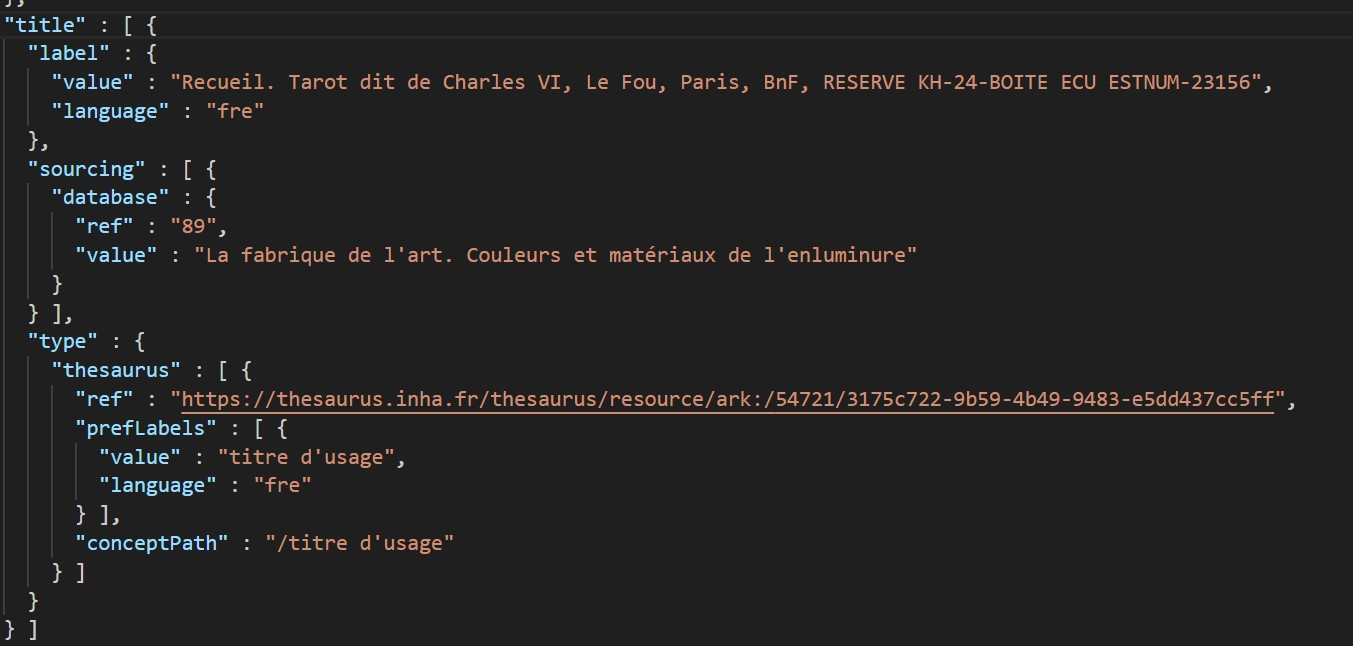
\includegraphics[height=8.02cm]{images_memoire/json_info_simple.jpg}
    \caption*{Extrait de notice au format JSON, pour les informations relatives au titre.\\
    Le chemin que le processeur suit pour extraire la chaîne de caractères constituant un titre est donc le suivant~:\\ \textsf{notice["content"]["identificationInformation"][‘’title’’][‘’label’’][‘’value’’]}.}
    \label{Extrait de code JSON}
\end{figure}

Régulièrement, le processeur se trouve devant une paire clé-valeur dont la valeur n’est pas une simple chaîne de caractères, ni même une autre paire clé-valeur imbriquée, mais une liste. Qu’elle qu’en soit la raison – il n’est pas souhaitable qu’une notice inscrive deux valeurs comme titre principal de l’œuvre –, il convient d’instruire au processeur d’examiner le contenu de cette liste, ce qui se traduit en Python par une instruction répétée autant de fois que la liste contiendra d’éléments, introduite par le terme \textsf{for}. Nous pouvons aussi, de fait, indiquer la position de l’élément visé au sein de la liste par son rang entre crochets, avant d’entrer le nom de la clé concernée. Mais cela peut s’avérer risqué au vu du caractère imprévisible du contenu d’une notice au format JSON.

Une fois l’intégralité des notices examinées, il est dicté au processeur de conserver comme résultat final l’ensemble des listes-conteneurs représentant chaque propriété d’un modèle de ressource, avec le contenu qui leur a été attribué par le script. Au terme de chaque section du script associé à une Classe arrive la dernière étape de transformation des données~: celle de leur exposition au sein d’un tableur CSV\footnote{Un tableur CSV \emph{(Comma Separated Values)} est un fichier de données textuelles où les valeurs sont séparées par des virgules, généralement utilisé pour stocker des données tabulaires, comme des feuilles de calcul, de manière lisible par l'ordinateur et facilement échangeable entre différents logiciels. On a parfois recours à un format cousin, le TSV (Table Separated Values), dont les données sont séparées par une tabulation.}. Chaque tableur créé par le script représentera l’ensemble des Contenus associés à un modèle de ressource dans Omeka. La méthode de création d’un tableur CSV \textit{ex nihilo} implique de définir au sein du script une liste de termes qui seront les noms des colonnes. Puisque une colonne représente une propriété, ces termes seront les noms des propriétés choisies lors de l’étape du \textit{mapping}. Une série d’instructions définit que chaque ligne sera représentée par une instance de la Classe dont on vient de définir le topique, et que chaque colonne chargera la liste-conteneur assimilée à la propriété qu’elle incarne. Cette dernière opération est à faire deux fois pour le tableur Couches, qui réunit deux classes ensemble. Au total, 1 cellule de ces tableurs CSV correspond à 1 propriété, appliquée à 1 instance de 1 classe. L’exécution du script génère ainsi 4 tableurs CSV par base de données.

\section*{2.3. Lancement de la base d’exploitation\protect\footnote{Toutes les opérations renseignées dans cette partie ont été tentées sous diverses formes à partir de juin 2023. Les derniers bugs empêchant l’initialisation du prototype d’Omeka S ont été résolus à la mi-août, alors que le stage était effectivement terminé.}}
\addcontentsline{toc}{section}{2.3. Lancement de la base d’exploitation}

\subsection*{2.3.1. Installation de l’environnement de travail de la base d’exploitation}

Nous avons évoqué le fait que le SNR développait ses infrastructures et outils d’aide à la recherche de manière collégiale, au sein d’un environnement de travail installé sur réseau, afin que chaque agent·e ait accès aux dossiers de configuration des divers projets qui l’impliquent. Il est donc prévu qu’à terme,  l’installation logicielle d’Omeka S s’opère sur le serveur central de ladite installation en réseau. Or présentement, au stade de la conception d’un prototype à des fins d’étude de faisabilité des demandes exprimées par le comité scientifique du projet Couleur – et ce à l’occasion d’un stage de fin d’études pour le département des Manuscrits – une telle installation n’est pas envisageable. En effet, toucher sans arrêt à la configuration d’une application installée en réseau peut causer des dommages en cascade difficilement réversibles~; il est préférable d’essayer de créer une première version sur un seul ordinateur, et ne généraliser le processus que lorsque l’on parvient à obtenir un résultat fonctionnel et sécurisé. De plus, du fait du statut de stagiaire de la BnF, l’accès aux outils techniques et aux bureaux de l’INHA n’est pas envisagé autrement qu’à fréquence exceptionnelle. Or la BnF, dont les ordinateurs font l’objet d’une politique de sécurité stricte de la part du Département des Systèmes d’information, n’autorise pas non plus l’installation de logiciels et d’éditeurs de code depuis le Web sur ses postes. Au total, la meilleure option est donc d’effectuer la configuration logicielle du prototype de la base d’exploitation sur ordinateur personnel.

L’installation d’Omeka S requiert une phase de configuration logicielle préalable, qui est celle de l’installation d’une machine virtuelle à destination de la création d’un serveur Web sur l’ordinateur. Car Omeka S est un logiciel de création de sites interactifs (ou \textit{dynamiques})~: et concevoir un site dynamique requiert de communiquer aux terminaux Web tout un ensemble d’informations depuis le disque de mémoire de l’ordinateur. L’ensemble des données composant les Contenus, mais aussi les documents HTML organisant l’affichage de chaque page du site dans le navigateur, les références de la base et les informations de connexion de l’administrateur·ice sont autant d’informations réparties au sein d’une kyrielle de documents, organisés en arborescence dans un unique répertoire – le répertoire \textit{racine} – qui sera manipulé par la personne propriétaire de l’ordinateur. Il convient donc d’organiser ces flux d’informations échangées entre ordinateur individuel et terminaux Web~; l’instance en charge de ce travail est le \textit{serveur Web}.

Ce logiciel permet de définir quel canal d’information (ou \textit{port}) traitera ses activités, quels protocoles seront suivis pour chaque type d’échange d’information, en bref de configurer l’espace d’activité d’Omeka S, afin que les autres tâches en cours sur l’ordinateur n’affectent pas ses propres compilations, et qu’à l’inverse, les diverses opérations effectuées pour Omeka S n’impliquent que les documents de son dossier racine, et n’aient aucune incidence sur le restant des programmes de l’ordinateur. Car un script erroné important des données à l’infini ne provoque que des dommages sur un disque de mémoire interne~; mais il est possible de limiter la quantité de mémoire allouée à une machine virtuelle, de sorte que si ce type de catastrophe devait se produire, l’environnement de travail arriverait vite à saturation, le processus s’arrêterait, et l’ensemble pourrait être reconfiguré sans endommager les données affectées au fonctionnement habituel de l’ordinateur.

Le logiciel de gestion de serveurs virtuels le plus utilisé pour des connexions Internet est \textit{Apache}, qui est entièrement gratuit et transparent sur les scripts qu’il exécute (ce qui définit l’\textit{open source}). Son rôle est d’assurer la bonne transmission des informations des terminaux d’Internet à l’ordinateur. Il travaille de concert avec d’autres logiciels, affectés à la gestion de bases de données et de fichiers d’application PHP, tels que \textit{MySQL} et ses variantes évoquées précédemment, ou le très répandu \textit{PHP My Admin}. Tous ces sont réunis en une même interface de travail~: un logiciel dédié à la gestion de projets de sites dynamiques hébergés sur serveur Web virtuel. C’est ce logiciel-là qu’il est nécessaire d’identifier, d’installer et de configurer avant d’aborder le téléchargement d’Omeka S. Il inclut d’emblée tous les logiciels susmentionnés, ce qui facilite ce travail~; mais il doit être adapté au système d’exploitation de l’ordinateur (Windows, Mac, Linux), sans quoi il n’effectuera pas certaines tâches, voire ne fonctionnera pas du tout.

L’ordinateur utilisé pour ce stage utilise un système Windows. Or Windows est un produit de la firme Microsoft, qui n’est pas disposée à laisser ses clients agir sur ses dossiers de configuration dans la plus totale liberté, comme c’est le cas pour le système Linux. Il faudra donc un gestionnaire de machine virtuelle compatible avec les impératifs de Windows. C’est le cas de deux marques~: \textit{Laragon} et \textit{WAMP}, sachant que Laragon propose deux versions du logiciel – une dite \textit{Portable}, qui nécessite moins de la mémoire du disque dur pour fonctionner, et une dite \textit{Full}, visant la maximisation de ses performances. Il est difficile pour de non-initié·es de déterminer à l’avance quel produit fonctionnera sans encombre. Nous pouvons toutefois observer dans les propriétés de la dernière version d’Omeka S ( la version \textit{4.0.1} en juin, puis la version \textit{4.0.3} installée en août) requiert des versions des logiciels PHP et SQL qui soient particulièrement performantes et récentes~: \textit{PHP 7.4, MySQL 5.6.4} ou \textit{MariaDB 10.0.5}. Or Laragon Portable n’implémente que les versions logicielles \textit{PHP 5.4} et \textit{MySQL 5.1}. Il en résulte que des tâches complexes, telles que les imports CSV à venir, sont initiées mais jamais abouties~: le gestionnaire de l’application n’est pas parvenu à coordonner des tâches aussi complexes\footnote{Ce problème était également rencontré sur les installations test opérées à l’INHA, mais pas systématiquement, sans doute du fait de l’habitude des ingénieur·es de mettre à jour les versions de leurs logiciels eux-mêmes. Si Laragon permet effectivement cela, mesurer précisément quelles fonctionnalités se trouvent corrigées, et quelles autres ne le sont pas encore, demeure difficile à notre stade de formation en informatique.}. La version Laragon Full, si elle propose la version PHP 8, se trouve encore limitée par une version de MariaDB qui est MariaDB 8. WAMP (la version 3.3.0) se montre donc plus compétitif, en proposant un panel de logiciels plus vastes, et suivant à peu près le rythme des évolutions des scripts~: \textit{Apache 2.4.54.2, PHP 8.0.26, MySQL 8.0.31, MariaDB 10.10.2, PhpMyAdmin 5.20, Adminer 4.8.1} et \textit{PhpSysInfo 3.4.2}. De cette cohorte de noms barbares, nous retiendrons que les versions présentées correspondent bien aux attendus d’Omeka S.

Leur installation est supervisée par WAMP, mais il s’avère qu’un ensemble d’opérations manuelles est nécessaire pour obtenir un environnement de travail adapté à ce que nous recherchons. À l’installation, Apache crée un profil \textit{administrateur} (le \textit{root}) qui dispose de tous les droits de téléchargement et d’exécutions d’applications\footnote{Ce qui est le cas pour toute initialisation du système d’exploitation d’un ordinateur~: Apache, qui crée des machines virtuelles, imite l’initialisation d’un nouveau système \textit{ex nihilo}.}. Mais cet administrateur n’est pas censé être associé à un projet en particulier~; il attend d’un projet d’être effectué par des profils \textit{utilisateur} créés lors de l’initiation de chaque logiciel. Or il clora par défaut les droits de ces derniers à lancer l’exécution d’applications, car cela \textit{pourrait} apporter des modifications à la configuration générale. Dans notre cas, il sera nécessaire d’autoriser plusieurs profils utilisateur à accéder aux fichiers, et exécuter diverses applications PHP. Nous devons donc manuellement modifier les droits d’accès au sein des trois fichiers suivants~:

\begin{itemize}
    \item En ciblant les lignes de code du fichier \textsf{C:\{\}wamp64\{\}bin\{\}apache\{\}apache2.4.54.2\{\}conf\{\}httpd.conf}\\

	\begin{minted}{php}
    <Directory "${INSTALL_DIR}/www/">
        AllowOverride None
        Options None
        Require all denied
    </Directory>
	\end{minted}

    Et en les remplaçant par~:
    
	\begin{minted}[bgcolor=codetab, tabsize=2, fontsize=\small, xleftmargin=5pt, xrightmargin=5pt]{php}
    <VirtualHost *:80>
        ServerName localhost
        ServerAlias localhost
    DocumentRoot "${INSTALL_DIR}/www"
    <Directory "${INSTALL_DIR}/www/">
        Options +Indexes +Includes +FollowSymLinks +MultiViews
        AllowOverride All
        Order deny,allow
        allow from all
    </Directory>
    </VirtualHost>
	\end{minted}

\medskip

    \item Et enfin les lignes du fichier \textsf{C:\{\}wamp64\{\}bin\{\}apache\{\}apache2.4.54.2\{\}conf\{\}original\{\}httpd.conf}, accorder la valeur \textsf{granted} à toutes les commandes \textsf{require}.
    
\begin{minted}[bgcolor=codetab, tabsize=2, fontsize=\small, xleftmargin=5pt, xrightmargin=5pt]{php}
	DocumentRoot "${SRVROOT}/htdocs"
	<Directory "${SRVROOT}/htdocs">
	Options Indexes FollowSymLinks
	AllowOverride All
	Require all granted
	</Directory>

	<IfModule dir_module>
	DirectoryIndex index.html
	</IfModule>
	
	<Files ".ht*">
	Require all granted
	</Files>

	<Directory "${SRVROOT}/cgi-bin">
	AllowOverride All
	Options None
	Require all granted
	</Directory>
\end{minted}
\end{itemize}

Le serveur WAMP part du principe qu’il peut être amené à héberger plusieurs projets de sites Web interactifs, et donc plusieurs logiciels d’édition de ces sites. Pour ne pas tout confondre, la procédure est de créer un \textit{Virtual Host} par projet~: un  répertoire créé dans le dossier racine, qui accueillera tous les dossiers nécessaires à l’exécution du projet. Comme pour tout logiciel, sa configuration initiale impliquera la création d’un profil administrateur disposant de tous les droits sur le projet, et de profils utilisateurs dont les droits seront variables, entre \textit{contributeurs} (droits de création, publication, suppression) \textit{éditeurs} (création, suppression, mais tout reste au statut Privé) et \textit{lecteurs} (accès en lecture seule). Nous créons donc pour ce projet un \textit{Virtual Host} du nom d’\textsf{omekas}, qui regroupera dans un même répertoire \textsf{omeka-s} tous les fichiers d’installation d’Omeka S.

\subsection*{2.3.2. Installation et configuration d’Omeka S}

L’installation d’Omeka S sur notre serveur WAMP s’effectue simplement via le téléchargement du fichier d’application depuis le site d’Omeka. Il arrive en format compressé~; le déplacer dans le répertoire dédié aux VirtualHosts de WAMP, soit \textsf{C:\{\}wamp64\{\}www}, et extraire son contenu, qui résulte en la création d’un dossier d’application complet. On le renommera simplement \textsf{omeka-s}, et il constituera le dossier racine de la base d’exploitation.

Il s’agit ensuite de rendre Omeka S coopératif. On aura besoin qu’il nous autorise à modifier ses fichiers PHP, et d’obtenir le compte-rendu des tâches effectuées et autres contenus de messages d’erreur. Il est nécessaire pour cela de modifier quelques fichiers manuellement.

\begin{itemize}
    \item Dans le dossier racine du projet (\textsf{C:\{\}wamp64\{\}www\{\}omeka-s}), modifier la première ligne du fichier \textsf{htaccess}, .\textsf{\textcolor{graycode}{SetEnv APPLICATION\_ENV ‘’production’’}}, en remplaçant \textsf{\textcolor{graycode}{production}} (on applique l’installation existante sans revenir dessus) par \textsf{\textcolor{graycode}{development}} (on veut voir ce que le logiciel se dit à lui-même).\\

    \item Dans le répertoire de configuration générale, créer la structure d’accueil centrale des données que l’on implémentera pour le projet, au sein du fichier \textsf{database.ini} (\textsf{C:\{\}wamp64\{\}www\{\}omeka-s\{\}config\{\}database.ini}). Il est prérempli avec des clés, auxquelles on ajoute les valeurs préfigurées par le SNR, afin que toutes les versions-tests installés sur différents postes puissent être accessibles par l’ensemble de l’équipe.

    \begin{quote}
    \textsf{\textcolor{graycode}{user = "LaFabriquedeL'Art"\\
    password = "Fabrique@SNR2023"\\
    dbname = "lafabriquedelart"\\
    host = "localhost" (le port qu’Omeka S utilisera pour charger des contenus en local, ne cherchera aucun serveur externe)}}
    \end{quote}

     \item Dans le même répertoire, le fichier qui réunit l’essentiel des clés de configuration de l’application Omeka S est le fichier \textsf{local.config.php}. On y apporte les modifications suivantes~:\\

    \begin{itemize}
        \item Remplacement de \textsf{\textcolor{graycode}{‘log’ => false}}, dans la box \textsf{\textcolor{graycode}{‘logger’}}, par \textsf{\textcolor{graycode}{‘log’ => true}}, pour activer le journal des tâches effectuées.\\

        \item Ajout de la ligne \textsf{\textcolor{graycode}{Omeka\{\}File\{\}Thumbnailer' => 'Omeka\{\}File\{\}Thumbnailer\{\}Gd'}}, dans la box \textsf{\textcolor{graycode}{‘serviceManager’ => [‘aliases’]}} (il faudra peut-être changer c paramètre, car il renvoie encore des erreurs), pour indiquer où seront regroupées les images numérisées, dans leurs différentes résolutions~;\\

        \item Changer la ligne \textsf{\textcolor{graycode}{'cli' => [ 'phpcli\_path' =>  ‘null]}} en \textsf{\textcolor{graycode}{'cli' => [ 'phpcli\_path' => 'C:\{\}wamp64\{\}bin\{\}php\{\}php8.0.26\{\}php.exe']}}, pour indiquer quel est l’emplacement du script PHP central de WAMP, afin qu’Omeka sache d’emblée quelle application prendra en charge toutes les opérations automatisées nécessaires à son fonctionnement. Sans quoi, il peut se montrer désaxé et dans l’impossibilité d’importer des fichiers depuis l’ordinateur.
    \end{itemize}     
\end{itemize}

\begin{figure}[!h]
    \centering
    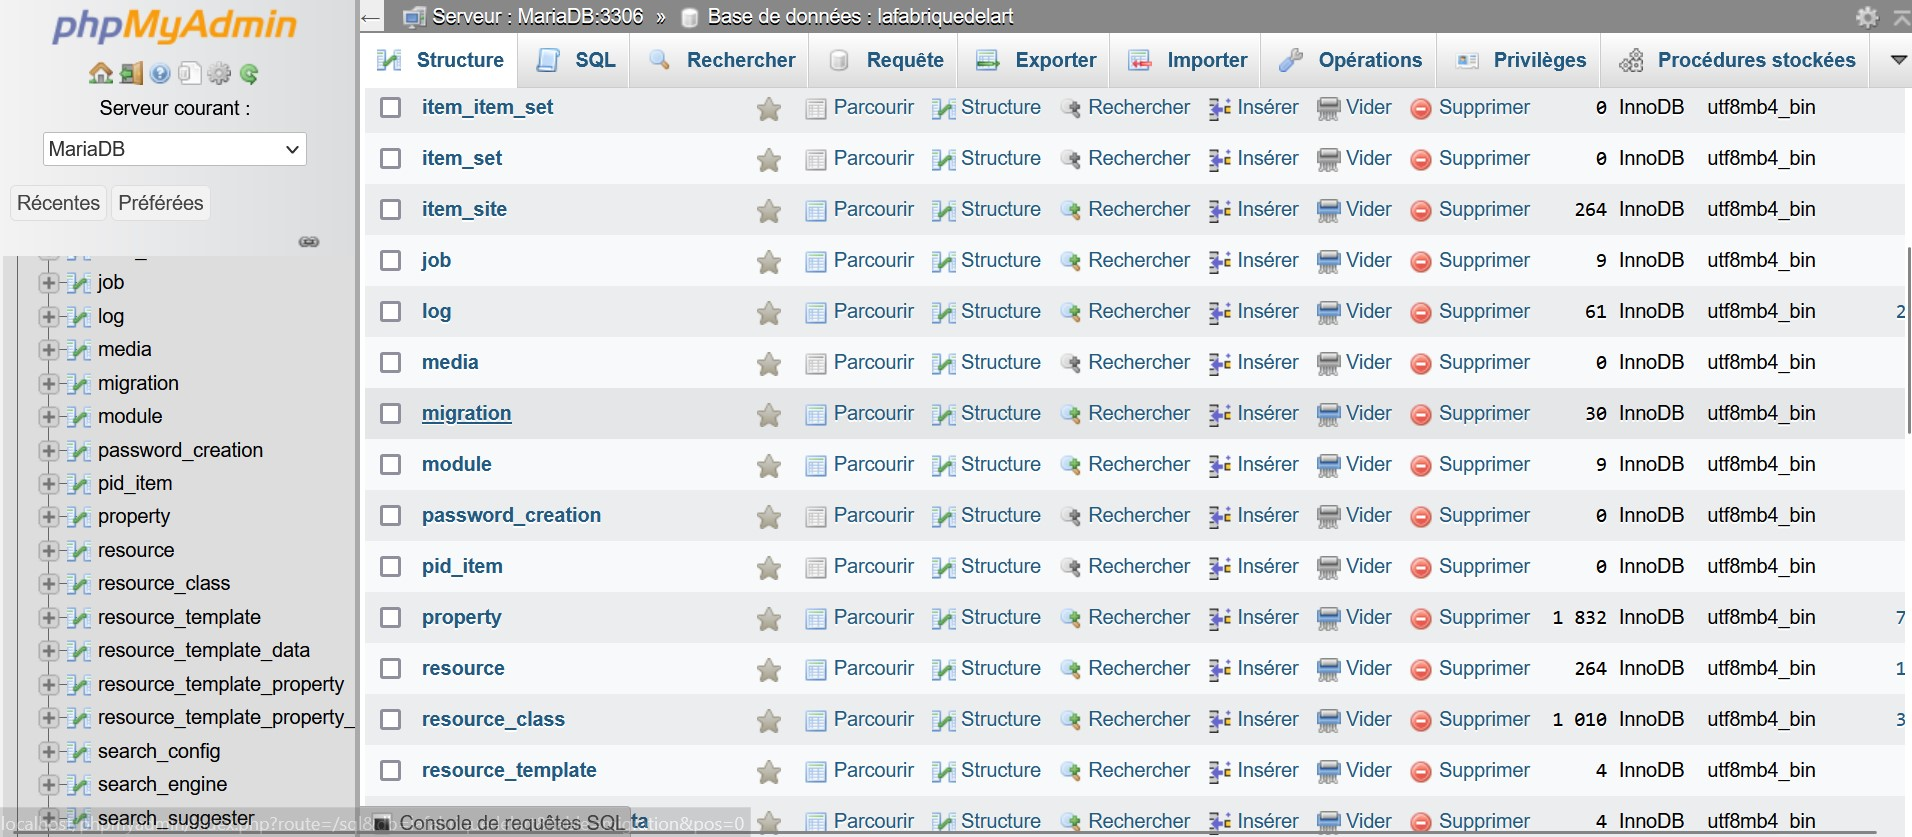
\includegraphics[height=7.35cm]{images_memoire/interface_phpmyadmin.jpg}
    \caption*{Interface administrateur du système de gestion de bases de données: MariaDB, dans le logiciel PHP My Admin.}
    \label{Interface de PHP My Admin}
\end{figure}

Ces changements apportés, la configuration de l’interface utilisateur d’Omeka S peut enfin être effectuée, avec la création d’un compte administrateur, le choix d’un thème graphique, et surtout des sites de présentation des futures ressources. On en créera donc deux, qui chacun comporteront leur propre ensemble de Contenus, et leur propre site Web de publication~; cette configuration reproduira donc de fait dans l’expérience utilisateur, et l’expérience des agent.es contributeurs manipulant uniquement le tableau de bord Omeka, la partition des deux bases.

\begin{figure}[!h]
    \centering
    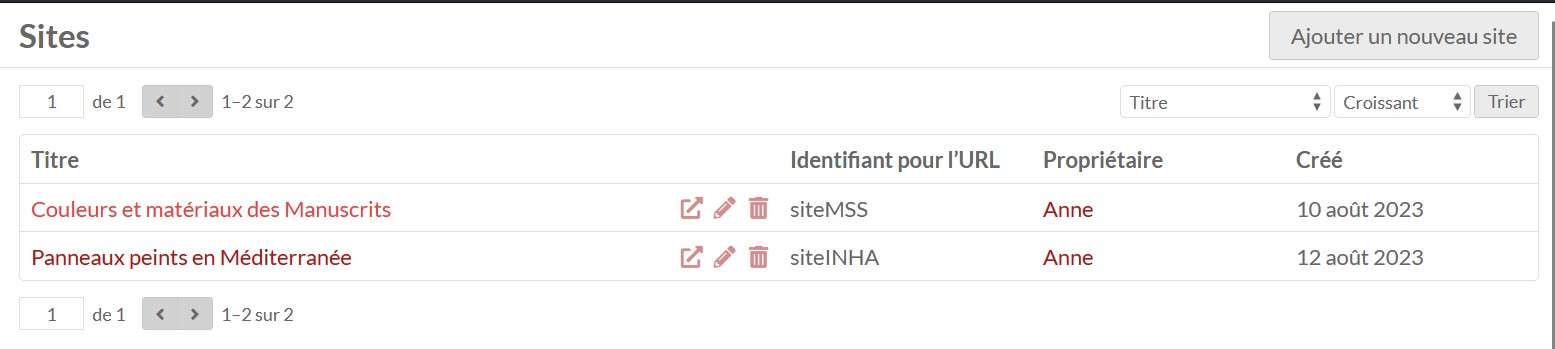
\includegraphics[height=3.77cm]{images_memoire/page_sites.jpg}
    \caption*{Recensement des sites sur Omeka S.}
    \label{Sites Omeka S}
\end{figure}

L’importation des vocabulaires des propriétés et définition des modèles de ressource s’effectuent à la main pour une primo-installation, ou peuvent s’opérer \textit{via} import CSV, si Omeka S pour le projet Couleur déjà été configuré sur un autre ordinateur. Dans tous les cas, il n’y a pas de spécifications techniques à apporter. Les dernières modifications manuelles interviennent lors de l’installation des modules, soit d’applications spécifiques à des fonctionnalités documentaires, qui comportent toutes les documents de configuration qui leur sont nécessaires. Il suffit de les choisir et les télécharger depuis le site d’Omeka au sein du répertoire \textsf{modules} dédié dans le répertoire source \textsf{omeka-s}\footnote{Il est donc relativement aisé d’ajouter ainsi des extensions au logiciel, ce qui ouvre un vaste champ de possibles quant à la possibilité d’en développer en interne.}. De ces modules disponibles, nous en comptons 6 qui deviennent rapidement indispensables à un bon fonctionnement d’Omeka S~:

\begin{itemize}
    \item \textsf{CSV Import}, dont dépend la possibilité d’effectuer nos dits imports de Contenus, au moyen des documents CSV créés par script, via des formulaires an langage naturel qui se chargeront de tous traduire en requêtes SQL eux-mêmes auprès de MariaDB~;\\

    \item \textsf{CSV Export}~: pas obligatoire, mais utile pour effectuer une sauvegarde de chaque site indépendante au format CSV (on peut aussi faire une sauvegarde de la base globale depuis MariaDB).\\

    \item \textsf{Resource Advanced Template}, qui permet d’exporter les modèles de ressources en CSV, et ainsi de se les échanger facilement entre contributeur·ices au projet~;\\

    \item \textsf{Log}, qui permet d’obtenir le bilan de chaque opération réalisée pour la configuration des ressources et du site, ainsi que le détail des messages d’erreur explicitant quels sont les fichiers concernés~;\\

    \item \textsf{Bulk}, qui aide à la modifications groupée de contenus de types de donnée différents. Se décline en deux modules de fait, \textsf{Bulk Import} (pour l’ajout) et \textsf{Bulk Edit} (pour la modification.) Nos bases associant des notices et des fichiers image, le module sera utile.\\

    \item IIIF~: module implémentant directement toutes les recommandations du standard comme fonctionnalités de la visionneuse fournie par défaut par Omeka. Il se répartit sur plusieurs modules~: \textsf{IIIF Server} (importation des fichiers image) \textsf{IIIF Viewer} (visionneuse), \textsf{IIIF Mirador} (ouverture automatique de l’image dans l’application Web Mirador.)
\end{itemize}

Quelques corrections manuelles au sein de MariaDB ne sont pas toujours évitables, comme celles du type de données de la colonne \textsf{message} de la table \textsf{log} de la base générale~: ce qui implique de remplacer la valeur \textsf{LONGTEXT} par défaut (qui s’attend à recevoir du texte libre, sans limite de nombre de caractères) par la valeur \textsf{BLOB} \emph{(Binary Large OBject)} qui désigne tout type de fichier binaire – donc de données brutes – sans discrimination. Parce que parfois, il ne semble pas reconnaître du texte, ou considérer que le message est trop long en dépit de tout (peut-être parce qu’il renvoie à de multiples fichiers du répertoire \textsf{omekas}, ce qui fait beaucoup de chemins d’accès à détailler.) Autant ne plus se poser de questions.

\subsection*{2.3.3. Importation automatique des données}

Un import CSV copie à l’identique le contenu d’une cellule~; il convient donc de nettoyer nos 8 documents CSV (4 par base Agorha, et par site Omeka S) des caractères typographiques qui résultent de leur traitement par script. Puisqu’il est question de données textuelles, cette opération peut s’effectuer par la sélection globale par regex, puis la suppression, de chaque type de texte concerné\footnote{Le détail des regex possibles pour cette tâche se trouve à la toute fin du script livré en document annexe.}. Il faut toutefois veiller, à l’ouverture du document dans l’éditeur, que le point-virgule ne soit pas compris comme un séparateur entre deux cellules~: il est utilisé dans Agorha pour séparer les valeurs d’un champ multi-valué, donc associés à une même propriété. Séparer la cellule à leur niveau revient à toutes les décaler d’un cran, et bousculer l’organisation générale en mettant des \textsf{Créateurs} dans des \textsf{Lieux de création}. Cela concerne les guillemets doubles, imposés dès la transformation des données Web d’Agorha en notices JSON pour renseigner des caractères, les guillemets simples mis par Python autour de chaque élément implémenté au sein d’une liste-conteneur, et enfin les crochets qui marquaient l’ouverture et la clôture desdites listes. De plus, l’INHA obéit à des consignes typographiques pour harmoniser ses documents CSV~: le séparateur au sein d’une cellule, qui signifient la présence de plusieurs valeurs à appliquer à une propriété, est le signe \textsf{\S}. Il convient donc de remplacer tous les points-virgules et virgules entre deux valeurs. La regex ne doit toutefois pas être appliquée aux colonnes du titre principal et du \textsf{Commentaire Matérialité}, car presque tous les titres utilisent des virgules pour concaténer diverses informations, et les \textsf{Commentaire Matérialité} demeurent des paragraphes entièrement écrits en langage naturel.

Le succès d’un import automatique dans Omeka dépend de plusieurs détails techniques~; les valeurs texte doivent pouvoir s’intégrer à la base \textsf{lafabriquedelart}, et y apparaître proprement. Ce qui nécessite que le document CSV, le logiciel Omeka S et le logiciel de gestion de \textsf{lafabriquedelart} MariaDB adoptent la même grammaire d’encodage des caractères. Pour s’en assurer, il est recommandé d’ajouter dans le fichier \textsf{database.ini} mentionné plus haut les lignes suivantes~:

\begin{quote}
    \textsf{\textcolor{graycode}{charset (langage de la structure de la base) = 'utf8mb4\_bin'\\
collation (tout logiciel qui travaillera avec) = 'utf8mb4\_unicode\_ci'\\}}
\end{quote}

ans MariaDB même, l’encodage général sera donc configuré sur \textsf{\textcolor{graycode}{utf8mb4\_bin}}, et l’encodage dit d’\textit{interclassement} (soit de dialogue avec d’autres logiciels) sur \textsf{\textcolor{graycode}{utf8mb4\_unicode\_ci}}. Ce n’est sans doute pas la seule option possible, mais puisqu’elle a le mérite de fonctionner, revenir sur ces modifications n’est pas une priorité immédiate.

Un import CSV est une tâche complexe, surtout lorsqu’il concerne un grand nombre de notices. Le processeur peut donc découper la tâche en plusieurs tâches initiées en parallèle\footnote{Comme Apache pour Windows est un programme \textit{multithread}, il ne lance pas un processus spécialement dédié pour chaque requête HTTP, comme il le fait pour Linux. Toutes les requêtes sont confiées à un seul processeur, qui arrivera donc trop rapidement à saturation tant que les fichiers de configuration ne l’aideront pas \textit{a minima} à déléguer quelques requêtes à d’autres processeurs. (documentation serveur HTTP pour Windows, URL~: \url{https://httpd.apache.org/docs/2.4/fr/platform/windows.html})}, ce que nous autorisons en ajoutant la ligne de code \textsf{\textcolor{graycode}{'Omeka\{\}Job\{\}DispatchStrategy' => 'Omeka\{\}Job\{\}DispatchStrategy\{\}Synchronous}} dans la box \textsf{\textcolor{graycode}{‘serviceManager’ => [‘aliases’]}}

\begin{figure}[!h]
    \centering
    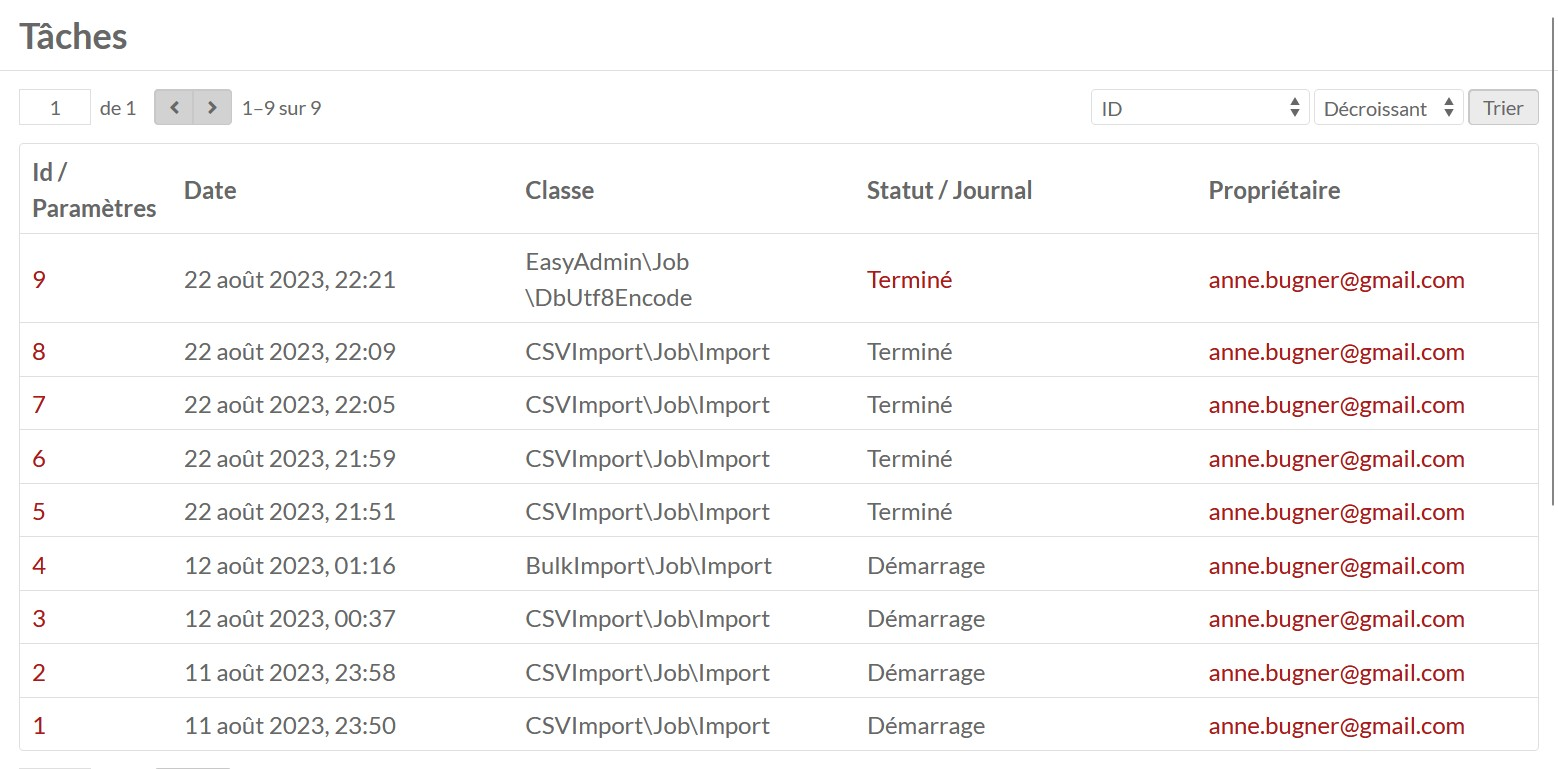
\includegraphics[height=8.29cm]{images_memoire/omekas_logs.jpg}
    \caption*{Journal des logs après de multiples imports: les statuts \textsf{Terminé} indiquent un succès, \textsf{Démarrage} un import dont les données étaient reconnues, mais que la superposition des tâches a mis en échec.}
    \label{Journal des logs après tentatives d'importation}
\end{figure}

La base générale dans MariaDB se compose de 48 tables. C’est dans la table \textsf{value} que l’on trouve nos \textsf{Contenus} exposés par Omeka S~: chaque ligne est une valeur d’un Contenu. La colonne \textsf{resource\_id} indique le numéro identifiant du Contenu où la valeur se trouve, et qui est créé automatiquement par Omeka lors de l’import CSV. La table \textsf{property\_id} donne le numéro identifiant de la propriété Web correspondante. C’est par des requêtes en langage SQL portant sur ces tables que l’on tentera, dans un chantier ultérieur, d’inscrire les liens entre deux Contenus.

L’environnement de travail des bases d’exploitation est donc lancé~; les opérations de configuration à venir vont concerner sa personnalisation. Le débat est donc ouvert à tous les niveaux de détail, que ce soit quant à la présentation visuelle de l’interface utilisateur, on des fonctionnalités de traitement des données des Contenus. Quelles représentations graphiques veut-on obtenir~? Quelles informations voudrait-on croiser~? Que va présenter la page d’accueil~? Comment assurer un fonctionnement simple, attractif, et néanmoins adapté à la formulation de questions complexes~? Comment va-t-on organiser les résultats d’une recherche~? Comment assurer aux visualisations des fonctionnalités interactives~? Comment encourager les spécialistes d’une discipline à considérer l’importance d’informations qu’ils ne soupçonnaient pas auparavant~?

Toutes ces interrogations nous appellent à sortir des machines virtuelles, terminaux et autres éditeurs de code -- bien qu’ils ne soient jamais bien loin, puisque nous en aurons besoin pour mesurer la faisabilité des idées envisagées -- et envisager le point de vue utilisateur des bases d’exploitation, en étudiant les méthodologies de recherche et les habitudes documentaires de leur public potentiel.

\clearemptydoublepage
\chapter*{3. Créer un outil de recherche de prise en main aisée pour des publics pluriels}
\addcontentsline{toc}{chapter}{3. Créer un outil de recherche de prise en main aisée pour des publics pluriels}

\section*{3.1. Enquêter sur les attentes des différents publics}
\addcontentsline{toc}{section}{3.1. Enquêter sur les attentes des différents publics}

\subsection*{3.1.1.Quelles communautés professionnelles~?}

Il existe bien des manières de définir des publics usagers de services culturels -- les ouvrages de bibliothéconomie sont pléthore sur le sujet. Par défaut, puisque le nôtre est librement accessible, son public est le \textit{grand public}~; tant qu’il n’est pas nécessaire de se connecter par un compte membre d’une institution, tout service documentaire en ligne est de fait \textit{grand public}. Mais puisque le nôtre entend être un outil d’aide à la recherche scientifique, c’est par la visée de leurs recherches que ses publics futurs se caractérisent~; recherches dont on peut au moins esquisser les contours en supposant qu’elles interviennent dans le cadre de leur activité professionnelle (ou étudiante) principale. Une première question évidente est~: \textit{Qui effectue des recherches en histoire de l’art~?}

Mais la réponse ne nous aidera pas~: l’histoire de l’art est en effet au cœur de nombreux secteurs d’activité culturels, et même d’entreprenariat privé, car elle participe à la valorisation d’un patrimoine matériel qui peut être une propriété privée~; ou, de manière plus ponctuelle, à la création de contenus de divertissement – on peut citer la documentation préalable à la mise en production d’un film en costumes ou un jeu vidéo, y compris à des fins purement esthétisantes. Quand bien même les recherches de toutes ces communautés professionnelles ne portent pas les mêmes impératifs de rigueur méthodologique, il est indéniable que les publics d’une base de données descriptives d’œuvres et objets d’art sont multiples, et auront des attentes différentes vis-à-vis de leur expérience utilisateurs, en supposant que le site d’Agorha et le projet Couleur soit portés à leur attention.

La lecture de périodiques professionnels dédiés à l’archéologie, l’histoire de l’art, la conservation préventive et curative, mais aussi à la gestion du patrimoine, viennent éclairer la caractérisation des domaines d’activité utilisant des ressources documentaires d’histoire de l’art, et à quelles fins. On peut actuellement esquisser les profils suivants~:

\begin{itemize}
    \item Le public cible de l’INHA, les historien·nes d’art (au niveau de chercheur·euses professionnelles ou doctorant·es), entendent utiliser un outil d’analyse quantitative à des fins herméneutiques~: il doit favoriser l’émission d’hypothèses nouvelles, et non se contenter de représenter des informations déjà connues, serait-ce à des fins pédagogiques ou ludiques. Les informations centrales ne sont pas tant les données descriptives, pour un travail universitaire, que celles explicitant leur processus d’obtention, et les limites intrinsèques qui en découlent pour l’appréciation de leur fiabilité. Comme source documentaire, la base de données doit être caractérisée, et rendre compte de la complémentarité de son approche au regard des autres sources convoquées pour les travaux de recherche.\\

    \item Le public cible de la BnF est de contours beaucoup plus élargis et flous. Spécialistes d’histoire de l’art bien sûr, puisque les manuscrits peuvent être considérés comme des documents iconographiques~; très proches en sont les chercheur·euses en histoire médiévale, byzantine ou de l’Islam – soit de toute période documentée par les collections, le service des Manuscrits médiévaux se concentrant principalement sur ces trois catégories. Plus rares en proportion, mais sans doute assimilés à des courants d’historiographie différents – qu’il serait pertinent de détailler – sont les spécialistes d’espaces non-occidentaux tels que le Japon ou la Corée, dont le service des Manuscrits médiévaux conservent effectivement des documents anciens. La contrainte que posent ces publics est celle de la visibilité des bases du projet Couleur au sein de l’offre générale pléthorique de ressources numériques que les institutions peuvent fournir pour la recherche en histoire médiévale. Une première réponse est d’encourager les renvois d’une ressource à une autre, comme Agorha le fait déjà en indiquant les liens vers les sites Joconde, Gallica, BnF Archives et Manuscrits, ou Biblissima~; une deuxième, autrement plus complexe, est de travailler au référencement du site au sein des navigateurs de recherche. La question reste ouverte.
    
    \medskip
    
    Mais de quel·les chercheur·euses est-il alors question~? Les spécialistes des corpus documentaires concernés, qui alors visiteraient les sites à fréquence régulière pour des recherches au long cours, quand d’autres opèrent dans le cadre de partenariats avec les sciences du patrimoine, ou pour les besoins d’un commissariat d’exposition, et donc utiliseraient la ressource pour le seul temps de leur projet~? Comment alors maximiser la qualité scientifique de la base, en explicitant les limites et démarches de l’obtention des données, sans prendre le risque de rendre les résultats incompréhensibles sous une surcharge d’informations~? Comment concilier les exigences d’études opérées à un niveau très fin (comme celles d’un style esthétique particulier), qui requièrent des réponses toujours plus techniques et spécifiques, et celles de travaux privilégiant de vastes ensembles documentaires, dont la définition repose sur la quantité de notices créées, où seules les caractéristiques les plus partagées importent~?
    
    \medskip
    
    Enfin, à l’heure où l’interdisciplinarité est vastement célébrée, quels tenant·es d’autres disciplines pourraient souhaiter consulter les ressources de la base~? Des spécialistes de Lettres modernes, pour le contexte sociologique et esthétique dans lequel s’inscrit la littérature européenne du XVIe siècle~? Des spécialistes de philosophie esthétique, justement pour comprendre le propos d’un style identifié, dans ses origines possibles et ses modalités de réception~? D’histoire sociale et d’anthropologie, pour l’étude rétrospective de la représentation de certains peuples, certaines pratiques de la vie quotidienne, certaines questions métaphysiques~? De géologie, pour enquêter sur l’évolution de la composition des sols d’une région~? (Après tout, l’usage de pigments minéraux a bien dû nécessiter de les extraire). Un examen automatisé de la myriade de données publiées par les plate-formes d’édition en ligne et des catalogues d’institutions, sur la base de leur travail d’indexation, donne un premier aperçu de ces publics improbables, mais pas impossibles, des ressources du projet Couleur, dont la formulation complète en langage naturel est un gage d’accessibilité.\\

    \item Cette accessibilité est une condition sine qua non auprès du public des étudiant·es, dont l’efficacité des méthodes de recherche personnelles n’est pas aussi rodée que celle des chercheur·euses professionnelles, et dont les habitudes documentaires sont forgées par les sites Web d’information en accès libre, dont la performance n’est plus à prouver, et les catalogues des services universitaires de documentation de leur établissement, dont la nomenclature est familière par sa représentation, quand Agorha en crée une propre à chacun de ses projets.
    
    \medskip
    
    La facilité d’accès, logistique cette fois – un chargement des pages rapide, une connexion du site Web stable, la possibilité de télécharger chaque ressource mise en ligne sur un ordinateur personnel – est un besoin partagé par étudiant·es comme enseignant·es, qui pourraient souhaiter utiliser les bases dans le cadre d’un exposé, sans risquer que l’accès aux ressources plante en plein vol. Si les modalités de téléchargement ressortent effectivement de la configuration des bases, nous ne pourrons toutefois pas nous prononcer sur le volume d’espace RAM (mémoire vive, utilisée par les processus des applications lorsque celles-ci sont ouvertes) alloué aux serveurs d’Agorha par l’INHA.\\

    \item L’INHA et la BnF sont également deux institutions particulièrement proches des professionnel·les du patrimoine~; l’une du fait de sa proximité physique avec l’Institut National du Patrimoine, haut lieu de formation initiale et continue des conservateur·ices, l’autre du fait de son statut de bibliothèque nationale, qui compte parmi ses missions d’être un établissement « tête de pont » auprès de l’ensemble des bibliothèques sous la tutelle du ministère de la Culture~; ce qui se traduit par la publication de recommandations diverses en matière de gestion des collections -- y compris patrimoniales – et de ressources pour leur valorisation scientifique, dont les travaux de recherche sur l’histoire de la production documentaire européenne font partie. Les conservateur·ices de bibliothèques patrimoniales pourraient donc profiter de l’enrichissement des ressources susceptibles d’inspirer des contenus de médiation scientifique, ou des prises de décision quant à la politique de préservation de leurs propres collections. Si ces dernières ont fait l’objet de collectes similaires, le site d’une institution publique d’envergure nationale peut être l’endroit où elles seraient le mieux valorisées, sous réserve que l’INHA accepte de convenir de conditions d’hébergement des données produites par d’autres acteur·ices. Enfin, pour l’exemple d’association de l’histoire de l’art à d’autres disciplines, cette ressource s’intègre aux missions similaires des conservateur·ices de musées, dont les pratiques documentaires ne font pas (encore) l’objet d’un examen spécifique dans le cadre du projet Couleur.\\

    \item L’ensemble des restaurateur·ices d’art constitue également un public potentiel, au regard du travail de documentation préliminaire requis pour la restauration des documents qui leur sont confiés\footnote{Voir ici l’annexe 4 de ce mémoire.}, que ce soit pour une restauration curative, ou leur préparation à une exposition. Ce qui pose d’emblée la contrainte de détailler avec clarté le niveau de chaque information donnée, pour que les prises de décisions soient faites en toute conscience. Une autre contrainte est de fournir une plus-value de fait sur les pratiques documentaires actuelles des professionnel·les. Ce peut être \textit{via} la performance de la base d’exploitation, qui alors leur éviterait un temps considérable de lectures multiples, d’ailleurs difficilement accessibles aux restaurateur·ices indépendant·es, en centralisant une quantité importante d’informations précises~; ce peut être aussi dans la recherche d’une complémentarité avec lesdites lectures multiples d’ouvrages documentaires de référence, en mettant en valeur les analyses physico-chimiques de documents atypiques, dont la diversité des techniques d’art identifiées témoigne d’un histoire agitée, et liée à de multiples provenances.
    
    \medskip
    
    Une contrainte d’un autre ordre impliquée par ces usages multi-professionnels est que la structuration sémantique des données soit particulièrement robuste~: les thésaurus doivent être non-ambigus auprès de toutes, régulièrement mis à jour, et disposer d’un mode d’accès \textit{pérenne} au plus possible~; les recommandations par bouche à oreille, lors de divers colloques, ne peuvent être efficaces si les ressources n’existent plus là où elles étaient initialement.
\end{itemize}    

\subsection*{3.1.2. Quelles méthodologies de recherche ressortent de ces différentes activités~?}

Chaque méthodologie de recherche a ses préférences en matière de mise en valeur de données en particulier. Il serait souhaitable de ne pas se limiter par défaut à celles des concepteur·ices des bases du projet Couleur, dans le souci de diversifier les publics, et d’obtenir des retours critiques constructifs sur les fonctionnalités proposées. Notons bien qu’il n’est pas question de choisir entre les différents procédés communiqués par les professionnel·les qui les emploient~; fournir un outil d’aide à la recherche revient à tenter de les rendre tous possibles, dans la mesure où les moyens techniques dont on disposent le permettent.

\begin{itemize}
    \item L’étude des œuvres en histoire de l’art, telle que pratiquée par les chercheur·euses impliquées dans le comité scientifique du projet Couleur, entend procéder du concret au conceptuel \textit{«~Je vois tel style esthétique. Où dit-on le rencontrer aussi, et quand~?~»}, de la perception immédiate à la reconstitution après observation \textit{(«~Ceci est une carnation, de couleur rosée~; or elle est conçue sur une teinte de base bleue ou de verte, ce qui suggère que la couleur des carnations n’appartenait pas aux registres des rouges, mais des ocres et des bistres~»\footnote{Termes de désignation des couleurs non contractuels})}\\

    \item Les réflexions des expert·es des sciences du patrimoine procèdent à partir de graphiques, qui sont les objets intellectuels dont on recherche les propriétés. Un composant chimique identifié, une technique d’application (broyages des pigments, épaisseur et nombre des couches, etc), définissent davantage les résultats d’une méthode d’analyse et les propriétés d’un phénomène physique général que le témoignage d’une activité humaine particulière. Elles renseignent ainsi également l’étendue des capacités d’un appareil, et sa possible complémentarité avec les autres qui ont été convoqués pour des analyses d’objets similaires.\\

    \item Les chercheur·euses historien·nes considèrent l’œuvre en présence comme une source documentaire, non un sujet d’étude en soi~; toutes ses données descriptives importent, pourvu qu’elles soient complémentaires aux autres sources primaires concourant au travail de recherche.\\

    \item Les chargé·es de collection du patrimoine partent des données documentaires à leur disposition pour en trouver d’autres qui pourront participer à l’enrichissement des leurs. \textit{«~Est-ce que nos objets viennent des mêmes régions que ceux présentés ici~? Est-ce qu’on leur trouve des caractéristiques communes~? Quelles campagnes d’analyse devrions-nous mener sur les nôtres~? Ont-ils plus de chance de comporter des matières colorantes d’origine végétale, animale ou minérale~? Quels sont les styles standards qui ressortent de ces enquêtes~? Les nôtres sont-ils en cohérence, ou plutôt porteurs d’un atypisme que nous devrions documenter~?~»}\\

    \item Les restaurateur·ices du patrimoine passent d’un point de vue à l’autre, en partant également de données documentaires lors de la phase de recherche préliminaire à l’arrivée effective des objets en atelier qui envisage les opérations de restauration à pratiquer. \textit{«~À cette date dans ce territoire, quels sont les matériaux support qu’on utilise~? Cette œuvre a-t-elle pu faire l’objet d’une transformation à une époque ultérieure à sa création initiale, et donc mélangé des pratiques artisanales de lieux et d’époque différents~?~»} Toutefois, la manipulation effective des œuvres peut faire ressortir des inconnues (une huile de lin qui n’a pas durci au séchage, un blanc de plomb ne s’étant pas oxydée dans la même teinte sur toutes les zones) qui amènent à émettre des hypothèses sur leurs techniques de création, et les processus de transmission et d’hybridation qu’elles ont pu connaître.
    
    \medskip
    
    Car le recensement et la caractérisation de ces modes de réflexion traduit directement le type de termes susceptibles d’être entrés en barres de recherche, et les champs de notices auxquels ils renvoient~: \textit{couleur, motif, période de création, titre, créateur}, etc. L’information recherchée – \textit{où trouve-t-on la même chose, quand, pendant combien de temps, pour quel type d’œuvre} – correspond aux modes de représentation graphique attendus~: par cartographie, chronologie – avec nombre d’occurrences ou non – ou encore diagrammes proportionnels. On peut ainsi concevoir des fonctionnalités de représentation graphiques qui répondent directement à des besoins documentaires, et des modes d’enquête.
\end{itemize}   

\section*{3.2. Quelles représentations graphiques pouvons-nous envisager à partir des données dont nous disposons~?}
\addcontentsline{toc}{section}{3.2. Quelles représentations graphiques pouvons-nous envisager à partir des données dont nous disposons~?}

Avançons-nous encore davantage dans le domaine des fantasmes scientifiques et ambitions techniques déraisonnables~; le travail de développement des fonctionnalités des bases d’exploitation doit bien se choisir une première direction. Nous regroupons donc l’ensemble des premiers modes de représentation graphique des données envisagés au fil des concertations avec les acteur·ices scientifiques du projet Couleur, en les classant par \textit{l’information centrale} à la requête.

\large \textbf{\textcolor{teal2}{Motifs}}\\

\normalsize
\begin{itemize}
    \item Cartographie des occurrences d’un motif sur une période et un espace donné~;\\

    \item Diagramme de tous les matériaux recensés pour la composition d’un motif donné (compter tous les matériaux de chaque couche d’un motif, et toutes les placer dans le même diagramme. Idéalement, le processeur serait en mesure de reconnaître les occurrences d’un même matériau parce qu’on ne donnerait pas tant son nom que son identifiant dans le (futur) thesaurus Matériaux de l’INHA.)\\

    \item \textit{Paramétrages nécessaires}~: la possibilité pour l’utilisateur·ice de configurer manuellement les bornes chronologiques souhaitées.\\

    \item Chronologie de l’évolution des motifs représentés au sein d’un type d’œuvre donné~: un graphique interrogeant les \textsf{Images} d’un certain \textsf{type d’œuvre}, leur période de création, et le nom des motifs liés à chaque \textsf{Image}. La visualisation serait alors un nuages de mots – les noms de motifs – dont la taille augmenterait avec leur importance~; et donner la possibilité d’apprécier l’apparition et la disparition d’occurrences, en associant au graphique une petite barre représentant les bornes chronologiques demandées, munie d’un curseur pour choisir une année, dont les données relatives s’afficheront en nuage de mots.\\

    \item \textit{Paramétrages}~: concevoir ce type de barre interactive, et le script de génération du nuage de mots autant de fois que les bornes chronologiques comptent d’années, ce qui pose la question de la limite des processeurs d’Omeka, et dans quelles conditions ce type de visualisation interactive est téléchargeable.
\end{itemize}

\large \textbf{\textcolor{teal2}{Visualisations des usages des couleurs}}\\

\normalsize
\begin{itemize}
    \item Fréquence des occurrences d’une couleur à une époque donnée~: croise le nombre de motifs iconographiques d’une couleur donnée et la période de création de leur \textsf{Image}. Le niveau d’information du \textit{motif} est préférable aux autres, si l’on cherche à documenter l’usage d’une couleur telle qu’elle est perçue par son public contemporain. Une Couche matérielle peut être d’une teinte qui n’est pas celle de la couleur visible \textit{in fine}~; une Image n’a pas de couleur directement renseignée~; de plus, les usages récurrents d’une couleur au sein d’une même œuvre picturale confirment sa popularité. Si l’interrogation porte sur l’utilisation d’une couleur en général, à tous les niveaux, c’est le nombre de Contenus \textsf{Couche matérielle} qu’il faudra alors compter. Reste à savoir comment permettre à l’utilisateur·ice de configurer cela à sa guise, sans devoir se confronter d’emblée aux concepts techniques de \textit{mixtion}, \textit{juxtaposition} ou \textit{assiette}.\\

    \item Coexistence de couleurs au sein d’une même \textsf{Image}~: or sont renseignées les couleurs qui ont fait l’objet d’une analyse physico-chimique. Il ne s’ensuit pas que \textit{toutes} les couleurs visibles sur une image aient bénéficié du traitement, encore moins si une couleur est récurrente, car la probabilité que les matériaux employés varie y est faible. Il n’y a pas eu de recensement de l’intégralité des couleurs visibles au sein de chaque Image inscrit au planning des contributeur·ices au projet Couleur.\\

    \item Détermination de la palette d’un artiste~: recenser les couleurs de tous les \textsf{Motifs} de toutes les \textsf{Images} attribuées à une même personne (personnes morales comprises)~; les représenter dans un diagramme circulaire, dont la part de chaque couleur augmentera avec le nombre de ses occurrences. Problème~: peut-on encore une fois considérer que ces occurrences sont représentatives~? Ou devrait-on simplement se limiter à l’affichage d’une palette où chaque couleur figure joliment dans un petit carré~?\\

    \item \textit{Paramétrages nécessaires}~:\\

    \begin{itemize}
        \item Permettre de sélectionner, au sein d’une \textsf{Image}, toutes les références aux \textsf{Motifs} qu’elle contient et dont la couleur est celle qui est recherchée, afin que les motifs concernés soient associés à une période de création~;\\

        \item Trouver un mode de représentation chronologique – donc une série de marqueurs individuels – pour renseigner des plages temporelles, sans créer de magma visuel infâme. La superposition de figures semi-transparentes, dont les dimensions seraient celles de la plage temporelle, présenterait-elle de meilleurs résultats~? Les mêmes considérations se posent pour les occurrences d’une couleur au sein d’une aire géographique donnée. Une option serait de délimiter les zones correspondant aux coordonnées spatiales par une forme semi-transparente, et apposer une étiquette donnant le nombre d’occurrences de la couleur recensée dessus.\\

        \item Rendre possible l’interrogation de champs avec la contrainte \textit{ET exclusif}, soit qui ne se contente pas de sélectionner les notices où la couleur A apparaît et celles où la couleur B apparaît, mais bien celles où les deux apparaissent \textit{ensemble}, et seulement celles-là. Attribuer à chaque valeur d’un champ couleur dans un Contenu de type \textsf{Motif} une couleur d’affichage (au format Hex Code, reconnu partout), en espérant faire le choix le plus consensuel possible.
    \end{itemize}
\end{itemize}    

\large \textbf{\textcolor{teal2}{Matériaux}}\\

\normalsize
\begin{itemize}
    \item Provenance d’un matériau (valable aussi pour la recherche de la provenance conjointe de \textit{deux} matériaux, voire davantage si souhaité). Il va de soi qu’ils n’auront pas tous été utilisés exactement au même moment, puisque les dates de création des œuvres ne sont jamais les mêmes. Donc il faudrait faire un fond de carte avec un grand curseur chronologique dessous, qui signalerait par étiquette l’emploi d’un matériau sur une aire géographique quand le curseur passe sur sa date de création. Si sa date de création est une plage temporelle, retenir la plus ancienne, ou faire une médiane~? Que faire~?\\

    \item Utilisation d’un matériau par une certaine technique (diagramme proportionnel renvoyant à une liste de notices où l’association figure)
\end{itemize}    

\large \textbf{\textcolor{teal2}{Techniques et savoirs artisanaux}}\\

\normalsize
\begin{itemize}
    \item Localisation géographique d’une technique donnée et évolution chronologique de l’emploi d’une technique donnée\\

    \item Qui nécessitera donc de nouveau le curseur d’exploration chronologique manuelle\\

    \item Technique et couleur obtenue (diagramme proportionnel de l’ensemble des couleurs obtenues pour chaque technique. Approche également valable pour l’interrogation croisée de la fonction de la couche en fonction de sa technique~?)
\end{itemize}   

\large \textbf{\textcolor{teal2}{Valeur économique du matériau en présence}}\\

\normalsize
\begin{itemize}
    \item Interrogation conjointe du matériau et de l’épaisseur d’une couche~: \textit{a priori}, un matériau étalé en couche épaisse ne fait pas l’objet d’un usage parcimonieux.\\

    \item Recherche de la mention de \textit{grains fins} ou de \textit{gros grains}~; plus un matériau est broyé finement, plus il fait l’objet d’un usage parcimonieux~;\\

    \item Recherche du nombre de couches constituant le motif~; la valeur serait alors ici le simple \textit{temps de travail} et de séchage.
\end{itemize}    

\large \textbf{\textcolor{teal2}{Degré de certitude en général}}\\

\normalsize
\begin{itemize}
    \item Provenances~: opacité de l’aire géographique délimitée par les coordonnées, croissante avec le degré de certitude.\\

    \item Matériau~: intensité de la couleur de l’étiquette associée.\\

    \item Possibilité de filtrer les résultats par degré de certitude souhaité
\end{itemize}  

\large \textbf{\textcolor{teal2}{Données de la conservation}}\\

\normalsize
\begin{itemize}
    \item Statistique des restaurations les plus opérées
\end{itemize}

\vfill

\section*{3.3. Chantiers envisagés pour la conduite du projet après le stage}
\addcontentsline{toc}{section}{3.3. Chantiers envisagés pour la conduite du projet après le stage}

\subsection*{3.3.1. Organisation d’entretiens et/ou d’ateliers auprès d’échantillons des publics potentiels}

Paris offre l’avantage indéniable de regorger d’institutions patrimoniales, laboratoire de recherche et d’universités de toutes disciplines. Il serait donc envisageable d’organiser des rencontres avec les professionnel.les disponibles au sein de toutes ces catégories. Un carnet d’adresses a été constitué, bien qu’il ne puisse être intégré ici pour d’évidentes raisons de caractère personnel des données. Nous pourrions imaginer deux types de rencontres, en fonction du nombre de réponses obtenues~: des entretiens individuels et personnalisés, ou des ateliers participatifs. Dans le premier cas de figure, nous échangerions avec un seul type de public à la fois, et aurions à enquêter de manière précise sur leurs habitudes documentaires et leurs limites. Ce qui revient à caractériser les informations recherchées, leurs modes d’accès et le temps alloué à ce processus. Il sera temps ensuite d’imaginer comment ces pratiques peuvent être optimisées.

Si les échanges promettent d’être fluides avec des professionnel·les de l’histoire de l’art, il n’en ira sans doute pas de même avec des historien·nes qui, bien que travaillant sur la circulation d’objets et de savoirs, ne dirigent pas particulièrement leurs recherches sur les pigments. Les entretiens peuvent donc aborder des thématiques voisines – l’identification de plantes ou de métaux participant à diverses préparations, par exemple – tant qu’il permet de comprendre le rôle donné aux outils numériques dans leur méthode de recherche. À quel stade de la recherche ces outils numériques sont-ils convoqués~? Servent-ils à susciter des hypothèses~? Des sujets d’intérêt~? Servent-ils de premier espace de test desdites hypothèses~? Viennent-ils en appui d’autres sources documentaires~? Sous quelles formes se présentent-elles~? A-t-on possibilité de les lier plus directement ensemble~? Quel choix est fait si elles doivent entrer en contradiction les unes envers les autres~? Servent-ils enfin dans les étapes finales, pour aider à la synthèse et la description des résultats finalement obtenus par les chercheur·euses~? Dans le cas d’une discussion avec des ingénieur·es de la donnée externes au projet, ce peut être en demandant sur quels critères leur expérience les fait mesurer la pertinence d’un nouvel outil numérique d’aide à la recherche, ou plus généralement, les projets de chercheur·euses qui au sein desquels leur rôle a été le plus déterminant.

L’organisation d’ateliers pratiques permettrait l’obtention en direct de retours utilisateurs, qui bénéficieraient de la synergie de groupe à l’œuvre, et serait susceptible de rendre compte de considérations que nos propres déterminismes de formation ne s’imaginaient pas. C’est une perspective tentante, mais déroutante par la quantité d’inconnues qu’elle implique – depuis le nombre de personnes répondant effectivement à l’invitation, la représentation proportionnelle de chaque type de public, les espaces qui pourraient accueillir une réunion exceptionnelle, et les outils dont ils disposeraient pour une communication. Imaginer également comment stimuler la réflexion collective \textit{via} une mise en situation adaptée, travail encore neuf en fin d’études de recherche, nous amènerait peut-être à considérer la littérature destinée aux entreprises~; après tout, il est bien question d’adapter un produit aux habitudes d’un groupe de personnes partageant un intérêt commun, qui est l’accès aux informations descriptives d’objets patrimoniaux du point de vue de leur matérialité.

\subsection*{3.3.2. Configuration avancée de la plate-forme Omeka S}

La personnalisation des bases d’exploitation est loin encore d’être à la mesure des attentes du comité de pilotage du projet Couleur en termes de prototypes~; manquent encore les fichiers image associés à chaque notice (et les visionneuses configurées pour le standard IIIF), et surtout les liens internes entre les Contenus, qui reproduisent la hiérarchie sémantique des niveaux d’information dans Agorha. Cette opération dépend de la prise en main du système de gestion de la base de données centrale d’Omeka S, MariaDB, et des requêtes dans le langage SQL. Le prototype de base tel qu’évoqué informellement par le SNR doit également comporter une API en mesure de mettre à jour les Contenus de chaque site automatiquement, sans passer par les étapes d’import CSV manuelles que nous avons détaillées ici. Omeka S prévoit en effet la configuration d’une API d’importation de données depuis une ressource externe, qui nécessitera, elle, une meilleure connaissance du langage de programmation PHP.

D’autres chantiers ont été évoqués, qui sont de fait réalisables dans l’architecture actuelle du prototype, mais sont secondaires au regard des précédentes, dont le fonctionnement effectif d’Omeka S dépend. Ils portent sur des points plus spécifiques, comme le sort à attribuer à la valeur \textsf{Null} des propriétés qui n’ont pas trouvé de valeurs renseignées dans Agorha~; qu’il s’agisse de ce terme ou d’une valeur vide, il serait souhaitable de configurer la propriété pour qu’elle passe au statut \textsf{Privé} – et donc invisible sur l’interface utilisateur – si elle ne renseigne rien~; ou la configuration des titres attribués à chaque ressource, qui par défaut sont limités à une seule propriété, ce qui rend particulièrement opaques les notices de motifs iconographiques et de couches matérielles. La mise au point d’une méthode précise pour quantifier le degré de certitude d’une information est également une opération qui paraît inévitable au regard des fortes attentes qui ont d’ores et déjà été exprimées sur ce sujet. La possibilité d’adjonction \textit{ad libitum} de pages dites \textit{statiques} à chaque site – soit de pages Web qui offrent seulement d’accéder à un contenu, et non de répondre à des requêtes – invite aussi à considérer l’ajout de contenus pédagogiques destinés à faciliter la compréhension des enjeux scientifiques du projet Couleur, telles que des références bibliographiques spécialisées en histoire médiévale, histoire de l’art et analyse des matériaux, ou des glossaires explicatifs des termes techniques relatifs aux méthodes d’analyse, dont les entrées seraient accessibles par clic depuis leurs instances dans les notices elles-mêmes. Les considérations relatives à l’optimisation du moteur de recherche, des fonctionnalités de représentation graphique, mais aussi au multilinguisme des sites, sont encore à discuter en groupes de travail.

Tous ces chantiers partent néanmoins de l’exploration des fonctionnalités de base, \textit{via} les modules proposés par le site d’Omeka S, afin de certifier qu’une version utilisable des bases d’exploitation pourra effectivement être ouverte au public dans les temps alloués au projet Couleur. Il apparaît donc que l’enjeu central au devenir des bases d’exploitation n’est pas tant dans les considérations informatiques, ou le recensement exhaustif de leurs potentialités ergonomiques, mais bien dans la priorisation des tâches que l’on voudrait voir effectivement abouties.

\clearemptydoublepage
\chapter*{Conclusion}
\addcontentsline{toc}{chapter}{Conclusion}

La création de deux bases de données permettant d’interroger ensemble les informations descriptives issues des inventaires des collections comme des rapports d’analyse en laboratoire représente un projet inédit dans la production documentaire de référence par les institutions. Il permet à l’ensemble des chercheur·euses du champ de l’histoire des cultures matérielles et des circulations de décrire sans ambiguïtés les tenants et aboutissants de leur travaux au moyen d’un vocabulaire thésaurisé commun, librement accessible et compréhensible par son soin du détail les relations sémantiques d’un terme spécialisé à un autre. Le choix des corpus de données inédites qui seront publiées au lancement de la base souligne cette ambition, en choisissant un espace aussi riche en circulations de personnes et de savoirs que le pourtour méditerranéen~; interface de multiples communautés ethniques et religieuses, il illustre comment des systèmes d’échanges perdurent de générations en générations, et créent un espace bien plus partagé que les concepts traditionnels historiographiques d’Orient, Occident, royaumes chrétiens et empire musulman le conçoivent initialement.

Le projet bénéficie des années de travail de formalisation des concepts de l’histoire de l’art opéré par l’INHA, qui permettent la convocation de vocabulaires d’une grande variété, et donc l’interconnexion d’informations qui ne sont pas réservées au domaine d’expertise des seuls concepteur·ices de la base. Le détail des fonctions assignées aux œuvres à travers le temps, de leur datation, leur provenance initiale – qui, même incertaine, sera toujours mieux supposée par le biais de l’analyse de leur composants que sans – de l’organisation de leur décor et des matières réunies pour leur fabrication touche aux intérêts scientifiques de nombreuses disciplines des sciences humaines, mais également des professionnels de la gestion du patrimoine, de la conservation, et de la production de contenus de médiation scientifique. Cette mise en partage interdisciplinaire de connaissances participe à la fois au projet scientifique de l’INHA, qui est de rassembler des données documentaires de provenances hétérogènes au sein d’un tout cohérent qu’est la plate-forme de publication et de mise en relation Agorha, et à celui des professionnel·les de la BnF, qui souhaitent encourager la préservation et l’utilisation en recherche des données produites dans le contexte de la gestion de la conservation du patrimoine.

Le pari du projet Couleur est de parvenir à développer un premier exemple effectif d’un tel outil numérique, dans le temps limité de trois ans (printemps 2021 – printemps 2024) déterminé par son inscription au plan quadriennal de la recherche de la BnF. Les étapes de sélection des corpus à faire analyser, de saisie des données issues des rapports d’analyse, de structuration de l’information pour Agorha, puis de personnalisation des modes d’interrogation et de représentation graphique sur base d’exploitation, sont donc appelées à s’effectuer quasi simultanément, au risque que les compromis effectués dans l’attente de la complétion de certaines tâches, dont l’exécution est plus lente (la conception de thesaurus dans la syntaxe du Web sémantique) endommagent la structuration formelle et sémantique des données. En effet, la caractérisation formelle de chaque donnée est la condition \textit{sine qua non} à son extraction ciblée, sa copie et sa redistribution dans l’architecture propre à la base d’exploitation finale du projet.

Or les opérations de réajustement sont possibles~: car l’ensemble des données des deux bases renseignent un nombre d’informations encore relativement restreint, de sorte que les décisions à prendre à leur sujet peuvent s’effectuer en réunissant l’ensemble des acteur·ices concernées rapidement, plus rapidement que pour des projets envisageant dès leur départ des ambitions documentaires très larges, et se heurtant en conséquence non seulement aux nombreuses incompatibilités de traitement, mais aussi à la difficulté de les résoudre en mettant d’accord tous·tes les expert·es des spécialités concernées, ne serait-ce déjà que pour obtenir tous leurs avis. C’est parce que le projet Couleur fait le choix initial de se concentrer sur les enjeux particuliers de deux projets de recherche -- les fonctions discursives et symboliques des livres religieux chrétiens du Moyen-Âge, les caractéristiques techniques des icônes peintes à la Renaissance, tous deux dans l’espace méditerranéen -- qu’il parvient à créer un système d’information cohérent, et que les \textit{process} suivis pour arriver au développement d’un prototype d’expérience utilisateur peuvent servir d’exemples. Ils instaurent un précédent en matière d’organisation des données de la matérialité des œuvres, qui peut être repris et adapté pour la description de collections de plus en plus variées – et ce, pour les espoirs juvéniles d’une apprentie chargée d’études, jusqu’à constituer une bibliothèque aussi éclectique et virtuelle que le labyrinthe imaginé par Umberto \textsc{Eco}, et riche de la même puissance évocatrice de la description détaillée des graphismes, couleurs et textures d’œuvres uniques.

\appendix
\renewcommand{\appendixpagename}{Annexes}
\appendixpage
\renewcommand{\appendixtocname}{Annexes}
\addappheadtotoc

\printbibliography[title=1. Bibliographie]
\addcontentsline{toc}{chapter}{1. Bibliographie}

\clearemptydoublepage
\chapter*{2. Répertoire des méthodes d’analyse physico-chimiques employées pour l’identification des matériaux}
\addcontentsline{toc}{chapter}{2. Répertoire des méthodes d’analyse physico-chimiques employées pour l’identification des matériaux}

\large \textbf{\textcolor{teal2}{Loupes et lunettes}}\\

\normalsize
Employées pour une première identification de \emph{composants organiques} présentant des structures visuelles répétitives caractéristiques,, comme les implantations de poil dans un parchemin qui identifient l’animal, ou les ramifications de fibres végétales. Sont également employées sur les décorations effectuées à l’\emph{or}, pour \emph{différencier les techniques} de feuille d’or et d’utilisation de poudres.

Convient particulièrement aux \textit{codices} dont le volume ne permet pas le passage au microscope. Méthode non invasive.

\large \textbf{\textcolor{teal2}{MO~: microscopie optique}}\\

\normalsize
Utilisé en priorité pour la caractérisation de \emph{matières vivantes} (toujours par le repérage de structures visuelles répétitives) et la recherche de marques de détériorations (lacunes, composition des poussières, etc).\\
Requiert de disposer d’une surface plane et fine, ou de prélever des échantillons. Méthode invasive.\\

\large \textbf{\textcolor{teal2}{MEB~: microscopie électronique à balayage}}\\

\normalsize
Technique basée sur le principe des \emph{interactions électrons-matière}, capable de produire des images en haute résolution de la \emph{surface d’une couche} (et donc d’observer sa granularité, ses disparités, ou l’absorption d’une couche par une autre)~; elle emploie également un \emph{détecteur EDX}, qui reçoit les photons émis par la matière suite à l’excitation électronique, et les trie suivant leur énergie pour caractériser les éléments chimiques en présence.

Opère sur échantillon. Méthode invasive.

\large \textbf{\textcolor{teal2}{Tests spécifiques de coloration}}\\

\normalsize
Passage d’un échantillon de liant sous \emph{révélateur} pour déterminer sa nature lipidique (huiles) ou protéinique (substances animales). Méthode invasive.\\

\large \textbf{\textcolor{teal2}{FORS~: Spectrophotométrie}}\\

\normalsize
Émission de des \emph{rayons UV} sur le support analysé. La \emph{longueur d’onde réfléchie} caractérise des éléments chimiques ; méthode convenant donc mieux à l’analyse de couleurs obtenues par pigments \emph{d’origine minérale}, et composés d’\emph{ions métalliques}, qu’à des des couleurs provenant de végétaux – par expérience pour des œuvres médiévales, les jaunes et verts (usages d’indigo).\\
 Méthode non invasive.

\large \textbf{\textcolor{teal2}{Méthodes d’analyse spectroscopiques par rayons X}}\\

\normalsize
Émission de \emph{rayons X} sur le support analysé. La \emph{longueur d’onde renvoyée} peut renseigner différentes opérations, selon les types de capteurs dont les appareils sont dotés. Cette méthode peut ainsi mettre en valeur les propriétés de \emph{fluorescence} propre à certains éléments chimiques (méthode \emph{XRF}) d’absorption de \emph{rayons infrarouge} (\emph{FTIR}), de variation de fréquence ondulatoires – complémentaire à l’approche par infrarouge (phénomène trop complexe pour moi, mais qui correspond à \emph{«~l’effet Raman~»}, et donc à la méthode d’analyse du même nom. Privilégiée pour les matières colorantes d’origine végétale, elle peut toutefois voir ses résultats faussés par les propriétés de fluorescence, que de nombreuses espèces conservent)~; ou les \emph{discontinuités de relief} (polymorphisme) au sein d’une couche, indiquant une éventuelle \emph{corrosion}, ou l’utilisation d’un pigment minéral broyé plus ou moins finement (\emph{XRD, WAXS}). Le type de rayons X émis conditionne certains paramètres, selon que les \emph{électrons (EDX)} ou les \emph{protons (PIXE)} y soient dominants.

L’ensemble de ces méthodes est apprécié pour sa \emph{polyvalence}, puisqu’elles permettent d’identifier finement des matériaux d’origine \emph{végétale comme minérale}, et de détailler la \emph{composition de couches de couleur}, ou les \emph{types de liant gras}, ou le \emph{degré d’oxydation d’un métal}. Elles opèrent également sur des zones d’analyses très restreintes (3 mm maximum), ce qui diminue la probabilité de mesures faussées par la présence d’impuretés.

En contrepartie, la \emph{manipulation} de leurs appareils est \emph{complexe} – le moindre mouvement écartent les capteurs de la zone d’analyse choisie. Le temps d’analyse nécessaire est de deux minutes minimum, ce qui peut contraindre les campagnes d’analyses menées sur des délais courts.\\
Méthodes non-invasives.

\large \textbf{\textcolor{teal2}{Radiographie par rayons X}}\\

\normalsize
Bien qu’elle permette la visualisation des \emph{niveaux sous-jacents d’une couche matérielle}, la contrainte d’une analyse sur support fin et plane rend cette méthode \emph{incompatible} avec le format de nombreux objets d’art, à commencer par les livres, qui devraient être \emph{massicotés}.

\bigskip

\large \textbf{\textcolor{teal2}{Source}}\\

\begin{quote}
    \small The conservation unit of the museums and galleries commission, \textit{Science for Conservators ,  Volume 1~:  An Introduction to Materials}, Conservation Science Teaching Series (London New York: The Conservation unit of the museums and galleries commission Routledge, 1992).
\end{quote}

\clearemptydoublepage
\chapter*{3. Revue de ressources Web - Bases de données relatives aux pigments, aux matériaux des manuscrits médiévaux, aux éléments iconographiques en histoire de l’art}
\addcontentsline{toc}{chapter}{3. Revue de ressources Web - Bases de données relatives aux pigments, aux matériaux des manuscrits médiévaux, aux éléments iconographiques en histoire de l’art}

\section*{Recenser des pigments}

\subsection*{\textit{Pigments Checker}~: un site polyvalent à destination de responsables de collections non physicien·nes, proposant des ressources pédagogiques comme des prestations payantes}

 \url{https://chsopensource.org/pigments-checker/}\\

 \normalsize Cet outil de recensement des matériaux utilisés pour la fabrication de couleurs, mis en ligne par le CHSOS, Cultural Heritage Science Open Source, un consortium italien. Il annonce d’emblée se concentrer sur les matières utilisées à l’époque moderne et contemporaine~; caractérisation des périodes d’usage certes vague, mais qui a le mérite d’exister. La page principale propose quatre types de ressources~:

 \begin{itemize}
     \item Plusieurs bases de données recensant de multiples spectroscopies, classées par méthode (XRF essentiellement). À chaque pic de la courbe d’un graphique est indiqué l’élément chimique en présence. Ces bases visent donc à aider les responsables de campagnes d’analyse à vérifier leurs hypothèses d’identification, pourvu que la méthode soit la même.\\

    \item Une liste de pigments synthétiques, de notre époque contemporaine, classés par couleur obtenue. Chaque élément comporte une petite notice qui recense son nom et les courbes affichées lorsqu’il est analysé via diverses méthodes de spectroscopie, dans la continuité de la visée d’une ressource documentaire d’aide à l’identification de composants chimiques, et des procédés colorants qui y sont associés.\\

    \item 9 bases de données image, qui rassemblent tous les graphiques utilisés pour les notices de pigments individuelles, par méthode d’analyse (FTIR, Raman 1064, Raman 830, Raman 785, Raman 532, XRF, FORS (deux fois), UV.)\\

    \item 2 exemples de photographies d’une analyse test, à partir d’une série d’échantillons de couleurs, dont l’observation est interactive~: l’utilisateur·ice peut glisser d’une vue (œil nu) à l’autre (observation UV et autres) et ainsi comparer en direct ce que chaque méthode d’analyse révèle.
 \end{itemize}

 Mais le site ne produit pas d’équivalent pour les matières naturelles~; et il ne prend pas en compte la composition des liants, supports et vernis. Il n’étend pas davantage ses réflexions aux usages de ces matériaux, que ce soit au sein de certaines œuvres, ou \textit{via} certaines techniques d’art.

 Enfin, ce site a une visée commerciale au moins aussi importante que ses services documentaires, proposant la vente d’appareils de mesure, de prestations d’analyses, ou des services d’expertise. Son but premier n’est donc pas strictement la recherche scientifique, mais l’aide aux professionnel·les et particulier·es responsables de collections d’œuvres d’art. L’accès aux ressources documentaires demeure toutefois gratuit, et ce tout du long de la navigation ( sans besoin de créer de compte, ou de payer pour en voir l’intégralité.) De multiples articles scientifiques anglophones sont également accessibles par exploration du site,  tous relatifs à l’analyse spectroscopique dans les sciences du patrimoine, et postérieurs à 2011, ainsi que des ressources pédagogiques inédites, comme les schémas explicatifs de 18 méthodes d’analyses patrimoniales, destinées à de non-physicien·nes.

 \subsection*{\textit{Spectra}~: un catalogue d’université}

 \url{https://spectra.chem.ut.ee/}\\

 Une ressource publique proposant un catalogue de pigments, liants et vernis a été produit par l’université de Tartu en Estonie. L’article détaillant l’histoire de ce projet peut se trouver ici~: \url{https://link.springer.com/article/10.1007/s00216-016-9411-5}. Toutefois, le nombre total de matériaux recensés reste conditionné aux données d’analyse disponibles aux équipes~; et de nouveau, la mise en relation des matériaux décrits avec les œuvres qu’ils composent n’est pas au programme.

 \subsection*{\textit{Pigments Database}~: une collaboration américaine entre divers acteurs de la chimie (universitaires, consultants privés), de la  physique et de l’industrie}

 \url{https://coolcolors.lbl.gov/LBNL-Pigment-Database/database.html}\\

 Ce site propose un panel plus vaste de pigments que ses précédents, naturels comme synthétiques (88 en tout), pointant chacun vers leur propre notice individuelle. Néanmoins, les graphiques d’analyse fournis se limitent aux méthodes de réflexion UV, et ne détaillent pas quel type d’appareil a été utilisé, ni l’interprétation des courbes, ce qui en fait un outil moins pédagogique que \textit{Pigments Checker}. Son originalité est néanmoins de documenter les propriétés du pigment selon la teinte de son support (noir ou blanc), ainsi que celles de certains mélanges (vert et rouge, bleu et blanc).

 \subsection*{\textit{Pictorials Materials Database}, un exemple esquissant l’association des pigments à un contexte historique}

 \url{https://www.centrorestaurovenaria.it/en/areas/diagnostic/pictorial-materials-database}\\

 Plus ambitieux, le projet de la ISTITUTO NAZIONALE DI RICERCA METROLOGICA, initié en 2017, (également complètement anglophone) qui documente environ 170 matériaux utilisés dans l’histoire de l’art pictural occidental.\\

Le projet entend \textit{reproduire} les matières colorantes utilisées à travers les âges, et ainsi montrer directement à quoi elles peuvent ressembler. Un pigment est donc sélectionné, et plusieurs types de peintures sont composés (avec deux liants ou plus) et étalés par touches sur un panneau préalablement enduit de stuc. Quatre panneaux sont en tout produits, chacun s’attribuant la mission de documenter une (large) période de l’Histoire occidentale. Trois panneaux sont dédiés aux pigments à usage picturaux (\textit{Antiquité, époque médiévale et moderne, époque contemporaine}) et un aux usages tinctoriaux.

Chaque échantillon de chaque panneau est indexé à l’unité, puis photographié sous diverses configurations~: sous lumière naturelle, puis sous divers filtres UV et infrarouges, dont les images sont placées en série au sein de la notice pour comparaison. Deux graphiques – un FORS et un XRF – complètent chaque notice. (\url{https://webimgc.inrim.it/Hyperspectral_imaging/Database.aspx})

Néanmoins, cette ressource ne fait pas de lien avec des œuvres particulières identifiées, ni des dates et des lieux de création, et encore moins des usages culturels. L’approche reste celle des sciences du patrimoine. Le lien avec l’histoire de l’art n’est fait que dans les articles scientifiques joints, non au sein de la base elle-même. L’article scientifique présentant le détail de cette base est là~: \url{https://link.springer.com/article/10.1007/s00339-017-1031-1}.

Un autre projet de reconstruction de peintures selon des recettes historiques, déterminées à partir de 70 analyses spectrographiques de la fresque de la Chapelle Sixtine, est présenté ici~: \url{https://hcommons.org/deposits/item/hc:29157/}. Les méthodes d’observation sont documentées de manière détaillée – notamment quant aux problématiques que posent les restaurations ultérieures pour la reconstitution stratigraphique de chaque œuvre picturale. Les résultats de ces analyses, publiés sous la forme d’un tableur organisé (3 colonnes~: \textit{échantillon / liant / notes}), pourraient presque assimiler la démarche documentaire à celle d’Agorha~; mais ce tableur est au format .pdf, et vient servir la lisibilité des résultats, non l’intégration à d’autres bases de données.

\subsection*{Une base de données des recettes des peintures recensées dans les sources écrites contemporaines à leur usage concret~: le projet \textit{ColorConText}}

\url{https://artechne.hum.uu.nl/node/9350}\\

Cette ressource entend réunir et contextualiser diverses recettes historiques de peintures . La plate-forme est co-dirigée par Sylvie \textsc{Neven}, spécialiste de la question et ancienne contributrice au Projet Couleur, (en tant que chargée de recherche sur l’année 2021.). La base recense des sources écrites, mais également l’ensemble des ingrédients mentionnés – qui obtiennent chacun une notice individuelle – et opère un système de renvois des noms anciens vers les noms actuellement utilisés. Chaque ingrédient constitue ainsi une voie d’accès au document-recette, dont les données documentaires (dates et lieux de création, auteurs, lien vers la notice institutionnelle, transcription du texte) sont bien mises en valeur. C’est ce qui s’approche le mieux de ce que nous recherchons~: cerner la présence de matériaux et de savoirs au sein d’un territoire donné, et en apprécier les mutations. Manquent toutefois les caractéristiques physico-chimiques des ingrédients – car un ingrédient n’est pas tout à fait assimilable à un matériau brut – et des liens avec les œuvres où ils se manifestent~; les documents-recettes sont des traités professionnels, non des commentaires esthétiques.

\subsection*{Des classements produits directement par les laboratoires~?}

\url{https://copa.hypotheses.org/552}\\

Certains rapports d’analyse en laboratoire concatènent ensemble leurs conclusions, en classant les graphiques d’observation par couleur, comme c’est le cas ici par le C2RMF. Toutefois, il s’agit bien d’un rapport d’analyse, s’adressant explicitement à des personnes familières des mesures opérées, et ne prenant pas la forme d’une base de données. Les pigments ne peuvent pas l’objet de requêtes individuelles (et ne sont pas associés aux œuvres analysées).

\subsection*{Une base de données dédiée à la seule méthode d’analyse RAMAN}

\url{http://www.irug.org/about-us/the-database}\\

Cette base est destinée aux professionnel·les des sciences des patrimoines, non des sciences humaines. Sa particularité est d’être indexée sur les graphiques d’analyse (qui constituent l’unité documentaire d’une notice), dont les matériaux qu’ils identifient ne constituent qu’une propriété parmi d’autres; approche sans doute utile à des utilisateur·ices qui n’auraient aucune hypothèse de départ quant à la signification de leur graphique. La liste des composants chimiques identifiés est publiée dans un onglet particulier du site (\url{http://www.irug.org/search-spectral-database/spectra-index}) Le site donne également la possibilité de rechercher directement à partir d’une molécule, ce qui confirme son public de chimistes.

\subsection*{Les ressources non scientifiques}

Le Web grand public n’est pas en reste, et n’est pas à sous-estimer dans ses ambitions totalisantes, à destination de praticiens amateurs – qui peut-être, voudraient reproduire les caractéristiques de maîtres admirés, ou combiner des matériaux trouvés à droite et à gauche sans produire de surprises chimiques désagréables. Un bon exemple est celui-ci: \url{https://www.artiscreation.com/Color_index_names.html#.XIBGq6B7mUl}. Le site réunit les informations relatives au nom commun d’un pigment, ses noms moins connus, son code commercial, sa composition chimique, son opacité, sa toxicité, sa résistance à la lumière, sa miscibilité avec l’huile, et quelques notes diverses relatives à ses usages dans l’histoire de l’art. La voie d’accès à une notice est par le numéro commercial du pigment recherché. Il s’agit là d’une base destinée à des praticiens de peinture à l’huile, non des chercheurs, qui chercheraient à en savoir davantage sur le matériel qu’ils utilisent. Étrangement, à part les publicités en bandeau, le site ne lie pas directement à la vente de produits.

Un autre exemple, dont la visée est documentaire, mais les contours méthodologiques un peu flous, est cette base~: \url{https://vplapps.astro.washington.edu/pigments}. Elle répertorie des pigments biologiques (comprendre~: végétaux ou animaux, dont la qualification de \textit{pigments} est d’ailleurs discutable), classés par ordre alphabétique, dans des conditions d’observations peu précises. Elle fournit néanmoins un premier répertoire de noms d’espèces biologiques susceptibles de fournir des pigments, ce qui constitue en soi une ressource pédagogique susceptible d’éveiller la curiosité des utilisateur·ices. Ce genre de curiosité se manifeste par exemple par des outils de recherche développés par des particuliers pour des usages personnels, comme celui-ci~: \url{https://github.com/rhockman/pigment_database}, script entendant extraire les informations relatives aux pigments au sein du catalogue de vente de peintures pour aquarelle Dick Blick, et les regrouper une base dédiée. (le catalogue en question est le suivant~: \url{https://www.dickblick.com/categories/painting/watercolor-paint/})

\section*{Bases de données iconographiques}

\subsection*{\textit{Mandragore}~: la base de référence des éléments représentés dans les enluminures, développée par la BnF}

\url{https://mandragore.bnf.fr/}\\

Il s’agit de la base de données (l’unique, au sein de l’éventail de ressources produites par la BnF) recensant les décors des manuscrits conservés par l’institution. Elle documente donc davantage de motifs que l’actuelle version de la base Manuscrits du projet Couleur ne peut le faire, car tous les manuscrits de la BnF n’ont pas fait l’objet d’analyses en laboratoire dont résultent des rapports au format numérique~; de plus, les bases du projet Couleur entendent décrire des œuvres issues de provenances diversifiées. Le contenu des deux bases est donc appelé à se différencier avec le temps. La base Mandragore propose 5 modes d’interrogation de ses données~:

\begin{itemize}
    \item Par cote documentaire ( ce qui permet une exploration des collections par arborescence en ouvrant un onglet dans le navigateur à chaque niveau, reproduisant le mode de navigation de BAM)\\

    \item Par sujet (Dictionnaire de sujets prédéfinis, qui est celui de l’enluminure entière)\\

    \item Par mot-clé, parmi un vaste ensemble classé par thématique – plus précisément des disciplines d’étude,\\

    \item Par recherche simple, le moteur de recherche demandant si le terme recherché est un mot-clé ou un sujet général, ce qui le renvoie sur les deux précédents~;\\

    \item Et par recherche avancée, où l’utilisateur·ice on peut additionner les termes recherchés, dans le but de rechercher la coexistence de motifs au sein d’une enluminure, ou limiter les résultats à ceux associés à des images numérisées.
\end{itemize}

Les résultats de recherche ne se contentent pas de fournir une liste de notices où les termes recherchés apparaîtraient~: ils classent toutes les informations disponibles par catégorie – listant donc toutes les cotes au sein desquelles le motif recherché est renseigné, les artistes illustrateurs, les titres, auteurs, siècles et lieux de création et thèmes généraux des textes concernés, ainsi que les autres mots-clés (motifs) inclus au sein de ces thèmes généraux. Assurément un modèle documentaire à reproduire pour les bases d’exploitation du projet Couleur.

Si ce type d’approche facilite la vue des variations sur un même thème, il ne va pas jusqu’à souligner le lien entre les informations de ces listes (qui figurent par ordre alphabétique) par exemple sous la forme d’un tableau à doubles entrées.

\subsection*{\textit{Photo-RMN}~: bibliothèque numérique de la RMN}

\url{https://www.photo.rmn.fr/C.aspx?VP3=CMS3&VF=Home}\\

Cette ressource est plus diversifiée dans les objets qu’elle documente, mais limitée dans les informations renseignées. Le moteur de recherche parse uniquement le champ \textbf{titre d’oeuvre} pour une requête de recensement des motifs visuels. L’indexation d’un motif visuel est donc conditionnée à sa mention au sein du titre de l’oeuvre, dont la grammaire est fluctuante.

\subsection*{Les bases \textit{Alma} et \textit{The Medieval Bestiary}}

D’autres exemples sont recensés par les services de documentation de l’EHESS, quoi que la liste mélange base de données de motifs et bibliothèques numériques~: \url{http://gam.ehess.fr/index.php?252}. Les bases Alma et The Medieval Bestiary proposent une indexation par motif, mais les liens URL vers les notices individuelles ne sont plus valides.

\subsection*{Base POP}

Elle centralise plusieurs bases de données iconographiques de collections patrimoniales, dont une «~Enluminures~», alimentée par divers établissements français, constituées à partir des années 1970, et centralisées et harmonisées sur un seul site à partir de 2018, sous la responsabilité du ministère de la Culture.

Les notices comprennent un champ «~Représentation~» qui qualifie la fonction générale de l’image («~Scène~») et place entre parenthèses, ensuite, une suite de termes relatifs au contenu visuel de l’image. Il est néanmoins facultatif. C’est parfois au champ «~Titre de l’enluminure / Sujet~» que revient ce rôle. La matérialité n’est toujours pas un sujet traité à part entière. Le champ «~Description~» pourrait remplir cette fonction, mais il est écrit en langage naturel, non en une suite de termes facilement extractibles, ou issus d’un vocabulaire contrôlé. Le champ «~Typologie du décors~» \textit{(sic)} liste, lui, une indexation formelle du type d’image en présence («~miniature, lettre ornée~») mais pas le contenu desdites images.

\clearemptydoublepage
\chapter*{4. Quelles attentes des publics potentiels des bases de La Fabrique de l’art~? Réflexions sur l’utilisation de la donnée par un public d’expert·es du patrimoine, à l’occasion de deux rencontres}
\addcontentsline{toc}{chapter}{4. Quelles attentes des publics potentiels des bases de La Fabrique de l’art~? Réflexions sur l’utilisation de la donnée par un public d’expert·es du patrimoine, à l’occasion de deux rencontres}

\section*{Analystes des propriétés physico-chimiques de manuscrits médiévaux}

Dans l’attente que le projet de base d’exploitation soit suffisamment avancé pour être en mesure d’expliquer de manière un peu précise ce qu’il permet de faire – exemples à l’appui, dans l’idéal – nous pouvons déjà nous rapprocher des chercheur·euses et professionnel·les du patrimoine qui ont publié sur la matérialité des œuvres d’art pour comprendre leurs démarches herméneutiques. Que souhaite-t-on \textit{voir}~? Quelles informations initialement invisibles – comme le sont les circulations passées des savoirs – pourraient être représentées, synthétisées, schématisées, à des fins pédagogiques~?

Si le mode opératoire le plus simple d’exécution pour ce type d’enquête demeure la lecture de travaux scientifiques publiés sur divers canaux, en espérant couvrir une diversité d’approches méthodologiques satisfaisante, la rencontre d’expert·es offre la possibilité de discuter de manière plus informelle de l’expérience concrète des outils d’aide à la recherche, et des particularités des informations du sujet. C’est aussi dans les récits empreints d’autodérision (une équipée rocambolesque pour accéder à des sources que plus personne ne pouvait localiser, des moments fastidieux de saisie manuelle de données avec des problèmes de lisibilité croissants avec leur volumétrie, ou d’incompréhension devant les documents d’autrui…), que l’espace des publications académiques ne privilégie pas, ou d’enthousiasme émerveillé (devant la découverte de sources documentaires imprévues, d’outils et de services de recherche pertinents au bon moment, ou l’efficacité au-delà de toute attente d’une synergie d’équipe pourtant mal amorcée) que l’on peut discerner les propriétés d’un \textit{bon outil} d’aide à la recherche. Un \textit{bon outil} ne se contenterait pas seulement proposer des données dont la rigueur de la structure permet l’utilisation au sein de travaux universitaires~; il répondrait aux besoins des usager·es lors de leur travail \textit{pratique} de recherche, lorsque chacun·e est ramené·e à ce que ses savoirs personnels lui permettent de faire en un lieu et un temps donné.

L’observation des expert·es de l’analyse physico-chimique d’ouvrages médiévaux, affiliés à l’université de Zurich, à l’œuvre au département des Manuscrits pour deux jours d’analyses XRF intensives sur certains éléments des collections, révélait déjà quelques légères difficultés strictement liées à une circulation de l’information entravée~; que ce fût par les systèmes d’identifiants concurrents au sein du document de rapport, ou l’hétérogénéité des langues employées pour désigner les éléments visuels à analyser, doublée d’un souci de concision parfois nuisible aux règles de grammaire (l’équipe était de fait quadrilingue, entre italien, allemand, anglais et suisse-allemand), dont résultait des ambiguïtés de traduction – voulait-on analyser le \textit{bord} d’un cadre (un contour bleu-noir), ou juste le \textit{cadre au bord} (d’un orange vif), quand un cadre était composé de plusieurs rectangles colorés~? Plus rarement, le nom d’un personnage pouvait avoir été indiqué par le chercheur responsable de la sélection du corpus et des zones d’analyse, sans détailler une localisation sur l’image ou d’attributs canoniques dans l’histoire de l’art, ce qui mettait en doute son identification au sein d’un groupe de figures. Or l’équipe prenait ses décisions non pas à partir d’autres sources documentaires relatives à ce type de figures, mais à partir du \textit{pigment que le chercheur pouvait estimer pertinent d’analyser}, au regard des autres zones analysées jusqu’à lors, et aux couleurs (verts, violets, noirs, mais peu d’orange) et matériaux (ors, pigments métalliques, qui pouvaient donner de l’orange) qui y étaient associés. Du \textit{pigment recherché}, on reconstituait la \textit{couleur recherchée}, pour ensuite identifier un \textit{motif significatif}.

Il en ressort qu’en présence d’une information manquante, les hypothèses de recherche s’orientaient vers ce que les propriétés du reste de l’ensemble documentaire pouvait suggérer, par calcul de probabilités, et que l’outil d’aide à la recherche idoine n’était pas l’examen détaillé d’un objet singulier, mais la mise à disposition d’une \textit{masse d’informations} propres à la comparaison. Le but de ces considérations n’est pas de juger de la pertinence de ces méthodes, ni même d’affirmer que nous avons identifié ici \textit{la} méthode dont cette équipe faisait usage~; le but est simplement de prendre en compte le fait que ce processus de pensée existe, et qu’à ce titre il est possible qu’il soit répété dans d’autres contextes, tout comme il est réel que cet équipe en adopte plus d’un différent pour ses prises de décisions à chaque moment de son projet.

\section*{Atelier de restauration en institution}

Une autre expérience marquante en matière de discernement des besoins auxquels une base de données numériques pouvait répondre, et aux modes d’optimisation qu’un outil facile de prise en main pouvait apporter, mérite d’être intégrée à cette réflexion sur les attentes des publics potentiels des bases du projet Couleur. Il s’agit d’une enquête menée en août 2020, dans le cadre d’un autre stage pour le département de la Conservation de la BnF, au sujet de la production et de la circulation des données de la conservation.

Interrogées au sujet des données les plus importantes à l’exercice de leur travail de restauration, les restauratrices de l’atelier \emph{Documents Graphiques et Maquettes} du département de la Conservation ont cité les matériaux des objets (particulièrement dans le cas de la présence de substances chimiques dangereuses~: il est dommageable de s’en rendre compte en direct), ainsi que les matériaux de leur conditionnement, qui en déterminent le mode de manipulation (absentes du travail mené par le Projet Couleur). Le niveau d’information souhaité allait jusqu’à la composition chimique précise des matières en présence, pour la facilitation du choix des solvants, et la prévention des dommages liés aux manipulations (exposition à la lumière, pression des remises à plat). Néanmoins, rares sont les rapports de laboratoire qui indiquent une formule chimique arrêtée~; les méthodes d’analyse soulignent la présence d’éléments atomiques, mais non leur structure moléculaire. Ce dernier point nécessiterait d’autres opérations d’analyse, évidemment coûteuses en moyens, et autrement plus invasive que les techniques de spectroscopie ne le sont.

Supposer la composition chimique d’un document à partir d’analyses de laboratoire menées sur des collections similaires constitue l’essentiel du travail de documentation préliminaire aux opérations de restauration. Il convient donc d’identifier lesdites collections similaires, et c’est pourquoi les données relatives à la provenance du document, sa date de création et ses pérégrinations antérieures à son arrivée dans l’établissement sont également vivement recherchées. Ce qui impliquerait, dans un monde idéal, la concaténation des données documentaires renseignées dans toutes les notices consacrées au sujet central d’une collection – que ce soit celles des objets, mais aussi des photographies qui ont pu en être prises, des catalogues d’exposition où ils apparaissent, des périodiques faisant état de leur acquisition.

Cette demande est de fait réalisable dans Agorha, au sein du bloc \textbf{Documentation~: bibliographies/archives}, qui est implémenté dans Omeka S par la propriété \textsf{dc:source}. Néanmoins, ces «~sources~» sont implémentées de manière indifférenciée. Une demande supplémentaire était d’indexer leur nature documentaire et leur date de publication, afin que les professionnel·les puissent les classer par ordre d’ancienneté (\textit{«~plus proche de l’état initial de l’objet~»}) ou de nouveauté (\textit{«~étude susceptible de fournir des éclairages nouveaux~»}). L’indication des niveaux de certitude relatifs à chaque information donnée était également revenue de nombreuses fois au cours des discussions.

L’évolution des contraintes organisationnelles de l’activité des restaurateur·ices, particulièrement la priorisation de la préparation d’expositions sur la restauration curative, tend à solliciter des restaurations en flux tendu au sein des ateliers, et donc à restreindre de plus en plus le temps alloué aux recherches documentaires préliminaires et à la vérification des informations renseignées dans les sources disponibles. Ces dernières, notices documentaires publiques mises à part, ne sont d’ailleurs pas directement accessibles, puisqu’elles concernent des documents professionnels internes aux services (dont la gestion de l’accessibilité sur l’intranet Lotus dépasse nombre d’agent·es) et des manuels sous format papier, provenant de bibliothèques ayant leurs propres contraintes de localisation, d’ouverture et de nombre d’exemplaires disponibles. La numérisation des ressources documentaires des sciences du patrimoine n’a pas bénéficié du même soutien que celle des universités.

Enfin, la restauration d’art, et encore plus au sein d’un atelier permanent rattaché à un établissement, peut être elle-même productrice d’informations inédites sur la composition matérielle d’œuvres et de documents, ou sur leur histoire passée~; le rapport de proximité entretenu avec les collections est précieux. Or partager cette information ne va pas de soi, puisque les temps de recherches préliminaires comme de rédaction des dossiers de restauration ne sont pas compris dans les devis renseignés aux chargé.es de collections. Ils représentent donc au mieux un défi perpétuel, et au pire une tâche parasite. La base d’exploitation devra donc pouvoir faire état de la diversité de provenance de ses informations, travail qui ne serait donc plus à refaire, ainsi que de leur niveaux de fiabilité. Toutefois, une contribution directe des professionnel·les de la restauration à l’alimentation des bases dans Agorha est inenvisageable, puisqu’elle viendrait se superposer au travail de rédaction des dossiers de restauration – évidence pour laquelle des contributeur·ices ont été spécialement recruté·es.

Toutefois, si la tendance à l’informatisation de ce processus se généralise, ainsi que l’uniformisation de la syntaxe employée (Lucile \textsc{Dessennes}, cheffe de l’atelier DGM en 2020, avait ainsi imposé avec succès deux modèles de dossier de restauration et de constat d’état des documents), il n’est pas exclu de recourir à des outils numériques pour reconnaître, extraire et transmettre les informations adéquates à Agorha. On peut penser à l’OCR, qui permettrait de reconnaître des termes récurrents à des emplacements similaires («~matériaux~:~», par exemple), et à des tables de correspondance entre les termes utilisés par chaque atelier et ceux du thesaurus publié par Agorha~; même s’il serait alors obligatoire d’en créer une propre à chaque atelier, en espérant que ce dernier ne change pas de modèle de document sans prévenir. De tous ces échanges, il ressortait donc l’importance de l’association des données relatives à la matérialité des œuvres avec leurs données descriptives documentaires, et la plus-value perceptive à court terme d’un outil de requête en ligne.

\clearemptydoublepage
\begin{landscape}
\chapter*{5. Tableur récapitulatif du \textit{mapping}}
\addcontentsline{toc}{chapter}{5. Tableur récapitulatif du \textit{mapping}}
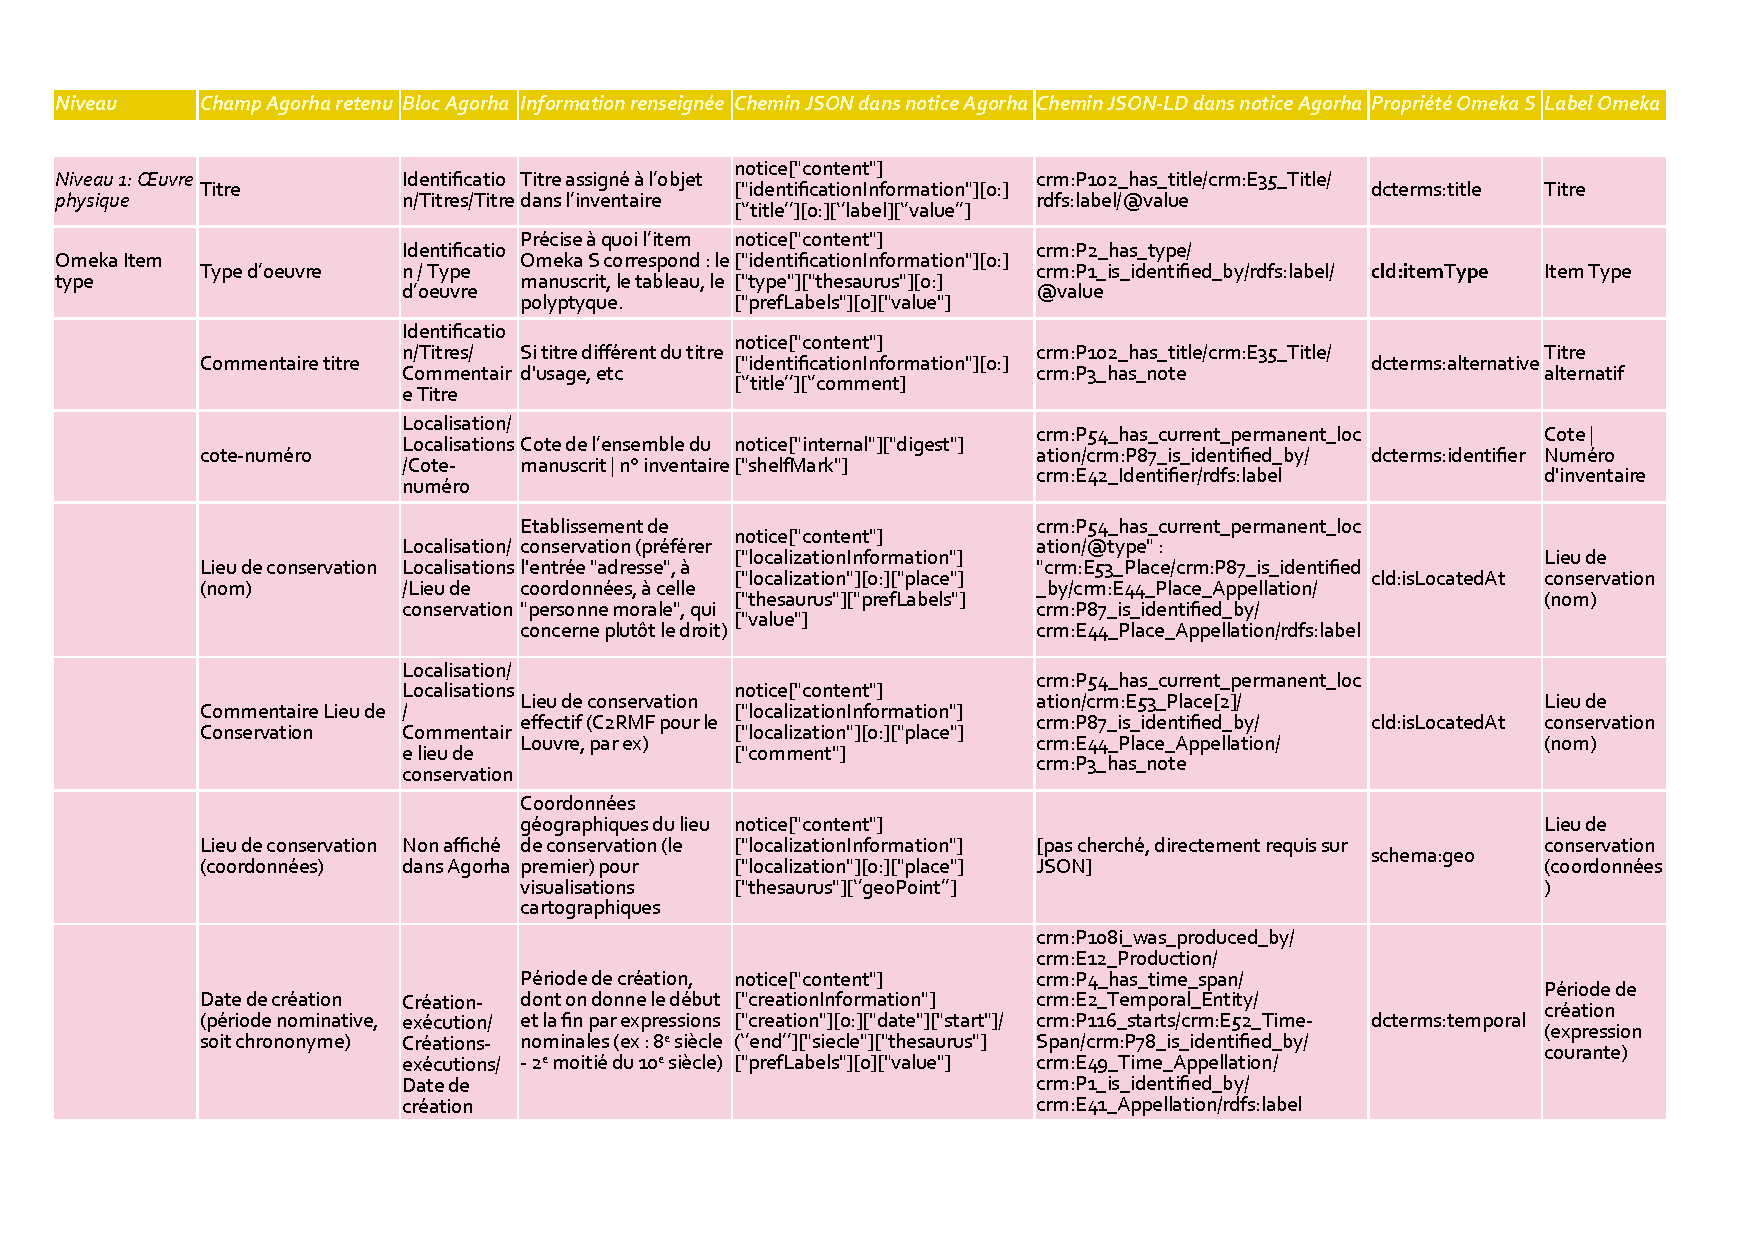
\includepdf[pages={1-24}]{projet_couleur_modele_ressource_omeka_1.0.pdf}
\end{landscape}

\clearemptydoublepage
\chapter*{6. Synthèse de l’état du projet à la fin du stage, à destination des tutrices M\textsuperscript{mes} Charlotte \textsc{Denoël} (BnF) et Emmanuelle \textsc{Bermès} (ENC)}
\addcontentsline{toc}{chapter}{6. Synthèse de l’état du projet à la fin du stage, à destination des tutrices Mmes Charlotte \textsc{Denoël} (BnF) et Emmanuelle \textsc{Bermès} (ENC)}

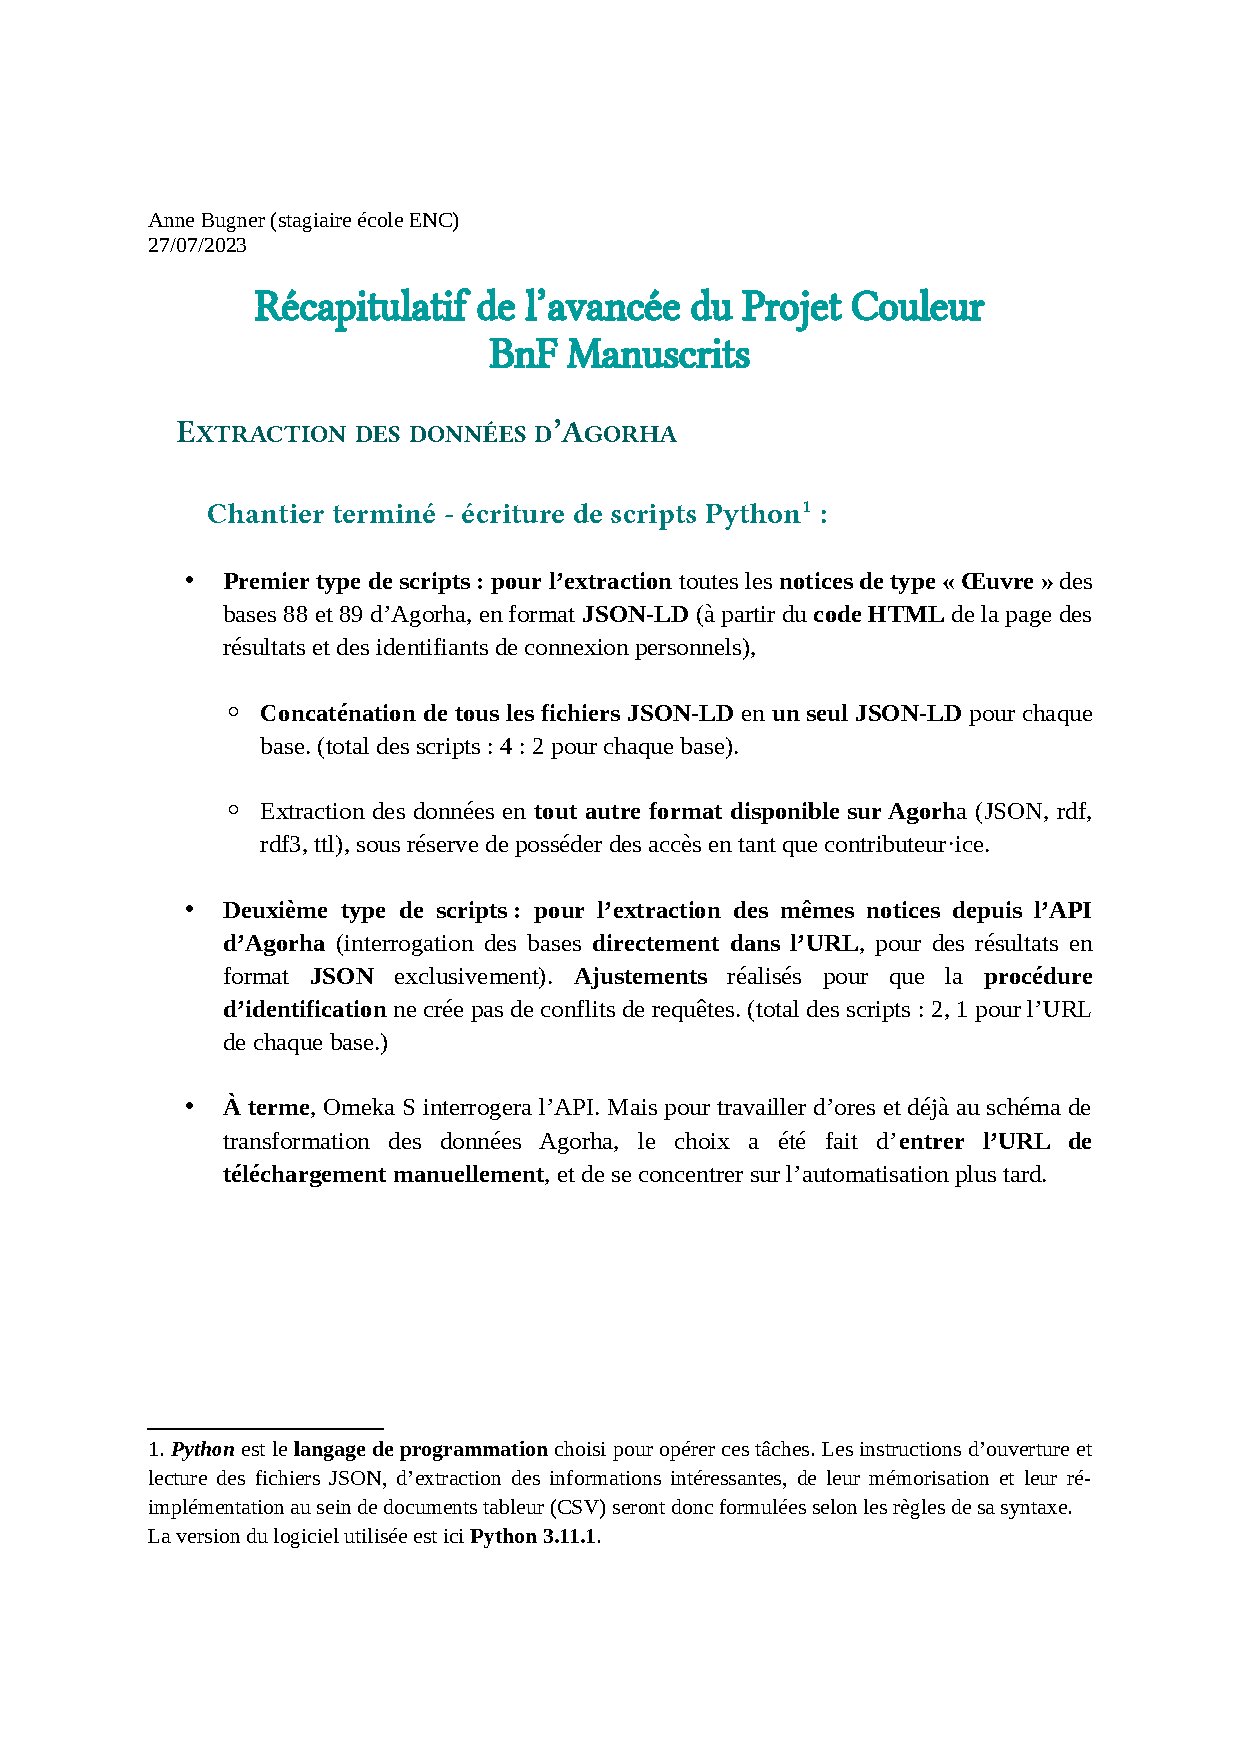
\includepdf[pages={1-8}]{synthèse.fin.stage.pdf}

\backmatter

\tableofcontents


\end{document}
